\chapter{Ruwe resultaten}
In dit deel word er over alle ruwe resultaten gegaan. Elke afbeelding in dit hoofdstuk bevatten rechtstreekse resultaten vanuit de XCode Profiler. Bij deze afbeeldingen word er ook een kort woordje uitleg gedaan die de resultaten beschrijven.

Voor het meten van het CPU verbruik tijdens het testen van verschillende methoden van data-overdracht is de Xcode profiling tool gebruikt met als template de CPU profiler. Met deze tool is gemeten hoeveel Mc(Mega cycles) de app vereist heeft van de CPU per type van data-overdracht. 

Voor het meten van het aantal updates van verschillende view property's, view refreshes en totale CPU gebruik tijd tijdens het testen van verschillende methoden van data-overdracht is de Xcode profiling tool gebruikt met als template de Swift-UI profiler. 

\section{test1: het testen op een lege view met grote dataoverdracht}
\subsection{CPU verbruik}

\paragraph{binding}
Uit de tabel blijkt dat wanneer we een binding gebruiken om een groot object door te geven aan een view, en we maken een aanpassing in die view, dit ongeveer 14,08 mega cycli van de CPU vereist.
\begin{figure}[htbp]
    \centering
    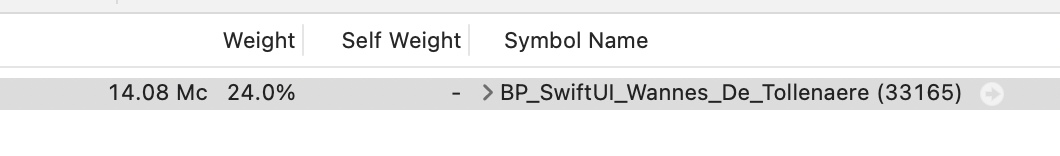
\includegraphics[width=1\textwidth]{BP_CpuUsageBinding} 
    \caption{test1: CPU gebruik van binding}
    \label{fig:cpuBinding}
\end{figure}

\paragraph{environment}
Uit de tabel blijkt dat het gebruik van Environment om een groot object door te geven aan een view, en het vervolgens aanpassen van dat object, ongeveer 250,08 kilocycli van de CPU vereist.
\begin{figure}[htbp]
    \centering
    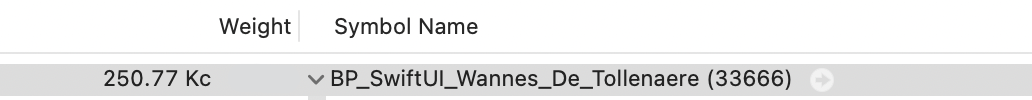
\includegraphics[width=1\textwidth]{BP_CpuUsageEnvironment} 
    \caption{test1: CPU gebruik van environment}
    \label{fig:cpuEnvironment}
\end{figure}

\paragraph{environmentObject}
Uit de tabel blijkt dat het gebruik van een environmentObject om een groot object door te geven aan een view, en het vervolgens aanpassen van dat object, ongeveer 17,13 mega cycli van de CPU vereist.
\begin{figure}[htbp]
    \centering
    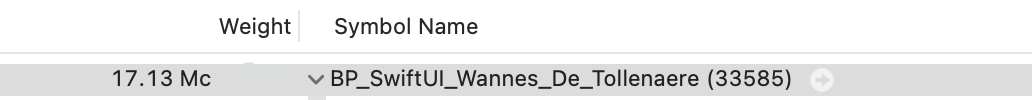
\includegraphics[width=1\textwidth]{BP_CpuUsageEnvironmentObject} 
    \caption{test1: CPU gebruik van environmentObject}
    \label{fig:cpuEnvironmentObject}
\end{figure}

\paragraph{observable}
Uit de tabel blijkt dat wanneer we een Observable gebruiken om een groot object door te geven aan een view, en we vervolgens een aanpassing aan dat object in die view maken, dit ongeveer 19,45 mega cycli van de CPU vereist.
\begin{figure}[htbp]
    \centering
    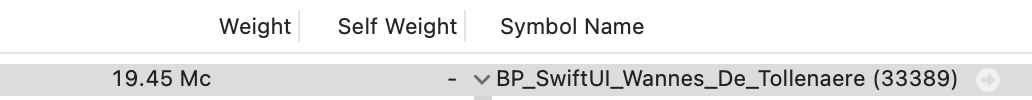
\includegraphics[width=1\textwidth]{BP_CpuUsageObservable} 
    \caption{test1: CPU gebruik van een Observable}
    \label{fig:cpuObservable}
\end{figure}\

\paragraph{observableObject}
Uit de tabel blijkt dat wanneer we een observableObject gebruiken om een groot object door te geven aan een view, en we vervolgens een aanpassing aan dat object in die view maken, dit ongeveer 17,82 mega cycli van de CPU vereist.
\begin{figure}[htbp]
    \centering
    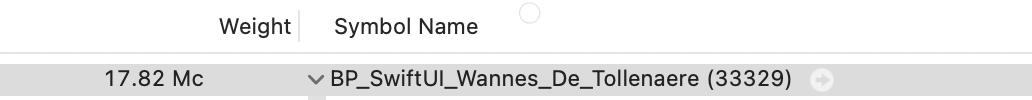
\includegraphics[width=1\textwidth]{BP_CpuUsageObservedObject} 
    \caption{test1: CPU gebruik van observableObject}
    \label{fig:cpuObservedObject}
\end{figure}

\paragraph{without property wrappers}
Uit de tabel blijkt dat het simpelweg doorgeven van een groot object aan een view zonder speciale annotaties, en zonder er vervolgens aanpassingen op te maken, gemiddeld 2,00 mega cycli van de CPU verbruikt.
\begin{figure}[htbp]
    \centering
    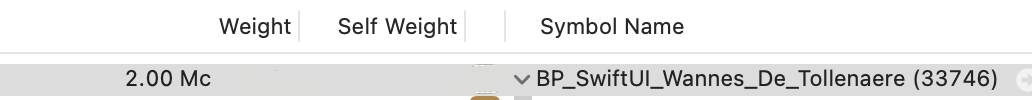
\includegraphics[width=1\textwidth]{BP_CpuUsageWithoutPropertyWrapper} 
    \caption{test1: CPU gebruik van een view zonder property wrappers}
    \label{fig:cpuWithoutPropertyWrapper}
\end{figure}

\newpage
\subsection{Property updates}
\paragraph{Snellere reactiesnelheid}
Binding, ObservedObject en EnvironmentObject passen de property bij elke wijziging tweemaal aan, wat zorgt voor een snellere en consistenter bijgewerkte state. Deze methoden zijn geschikt voor applicaties waarbij real-time gegevensuitwisseling en een directe reactie op veranderingen essentieel zijn, zoals een chatapplicatie of een live-dashboard.

\paragraph{Tragere reactiesnelheid}
Daarentegen voeren Observable en Environment slechts één update per aanpassing uit, wat kan resulteren in minder efficiënte of langzamere reacties op veranderingen. Deze methoden kunnen beter geschikt zijn voor applicaties waar updates minder frequent zijn of waar de responsietijd minder kritisch is, zoals een notitie-app of een takenbeheer-app.


\begin{figure}[htbp]
    \centering
    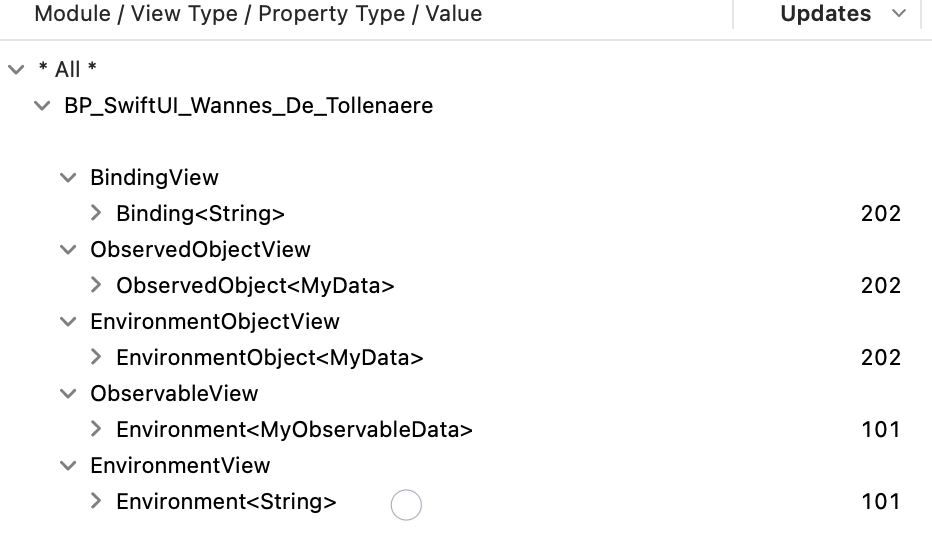
\includegraphics[width=1\textwidth]{BP_ViewPropertyUpdates} 
    \caption{test1: Aantal keren dat de property's geupdate zijn bij het 101 keer opnieuw toewijzen}
    \label{fig:propertyUpdates}
\end{figure}

\newpage
\subsection{View refresh time}
Voor het meten van het gemiddelde view refresh times van SwiftUI Views tijdens het testen van verschillende methoden van data-overdracht is de Xcode profiling tool gebruikt met als template de SwiftUI profiler. De resultaten zijn waargenomen door een view aan te maken, de data door te geven volgens de methode die aangegeven is. Vervolgens de data updaten. Dit 100x herhalen voor elk type View. Ten slotte de gemiddelde tijdswaarden aflezen in de Xcode profiler.

\begin{figure}[htbp]
    \centering
    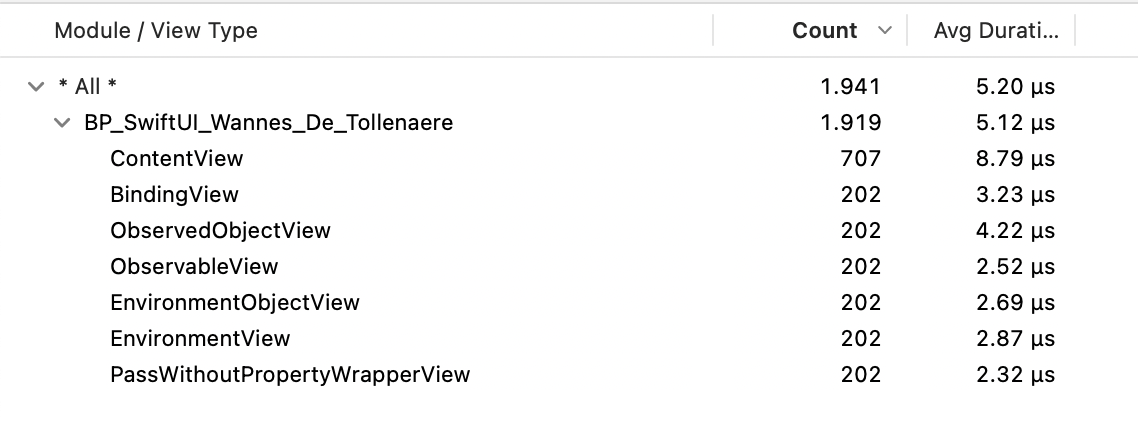
\includegraphics[width=1\textwidth]{BP_ViewRefreshCountAvgDuration} 
    \caption{test1: Gemiddelde duratie voor de view om in te laden per property type}
    \label{fig:propertyRefreshDuration}
\end{figure}

\section{test2: Dataoverdracht in subview's}
In dit hoofdstuk word de applicatie in de afbeelding hieronder gebruikt om de testen uit te voeren. Opgebouwd uit 1 VStack's die 10 HStack's bevat per HStack worden er 10 Tegels weergegeven. Elke tegel is zeer CPU heavy opgebouwd zodat de resultaten meer zichtbaar worden in de testen. Elke tile bevat ook een knop die een aanpassing van de testbare data gaat triggeren. In volgende afbeelding word de hierarchy afgebeeld. Voor elk type van dataoverdracht is er 10 keer op de button gedrukt voor het wijzigen van de view. Zo zijn de metingen tot stand gekomen. Alle ruwe resultaten die waargenomen zijn per datatype kan u terugvinden in onderstaande sectie's en afbeeldingen. 
\begin{figure}[htbp]
    \centering
    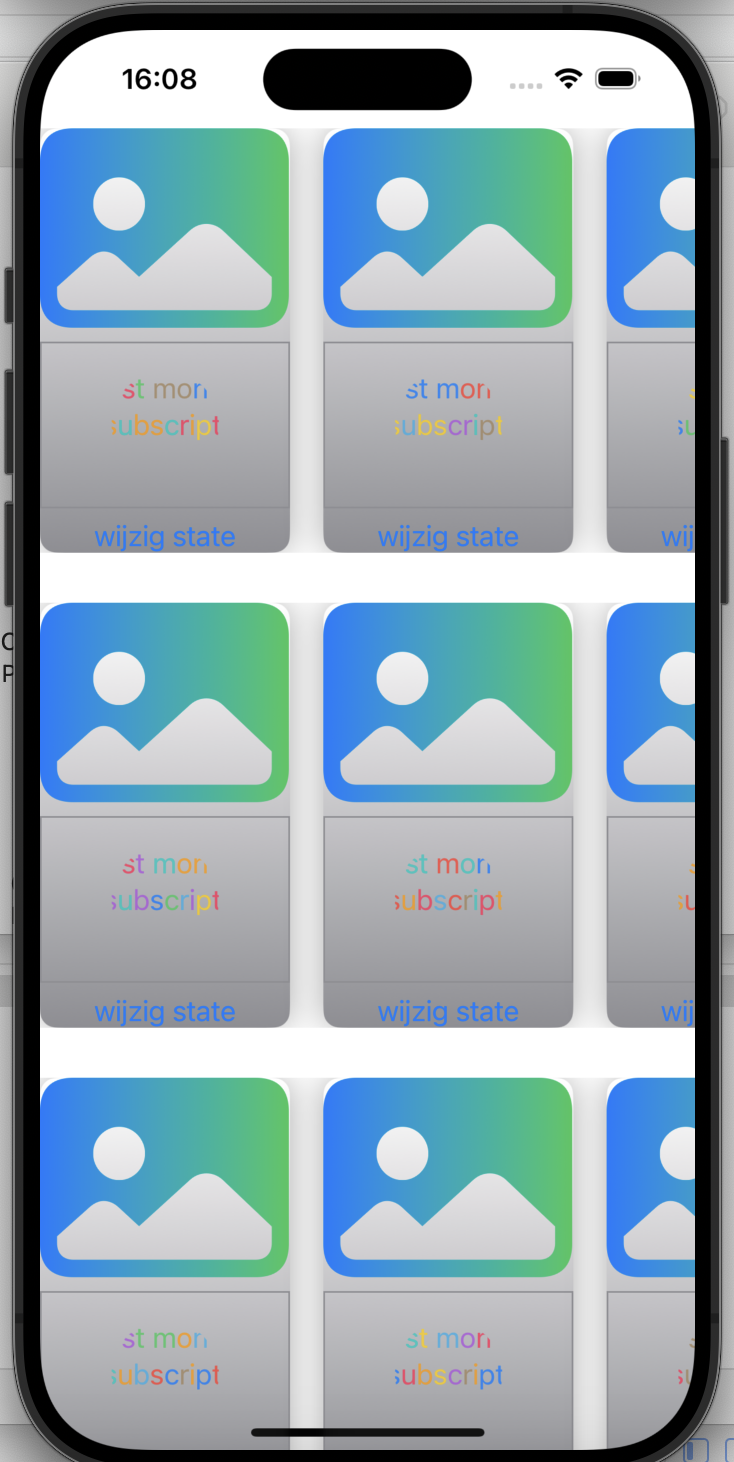
\includegraphics[width=0.4\textwidth]{testapplication} 
    \caption{testapplicatie}
    \label{fig:testapplication}
\end{figure}
\begin{figure}[htbp]
    \centering
    \includegraphics[width=0.4\textwidth]{bptest1_insubview/dataHierarchy} 
    \caption{testapplicatie data hierarchy}
    \label{fig:testapplicationHierarchy}
\end{figure}
\subsection{Samengevat}
Onderstaande tabel bevat alle samengevatte resultaten uit deze test.
\begin{figure}[H]
    \centering
    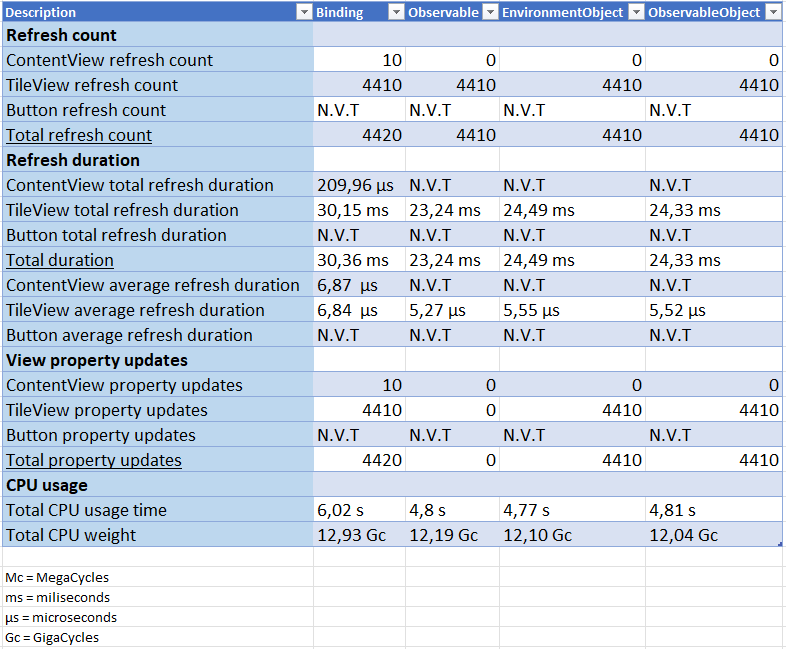
\includegraphics[width=1\textwidth]{bptest1_insubview/resultstable} 
    \caption{resultaten tabel}
    \label{fig:resultatentabel1}
\end{figure}
% Binding test 1
\subsection{Binding}
\paragraph{View ververs aantal en ververs tijd }
%viewrefreshtime
\begin{figure}[H]
    \centering
    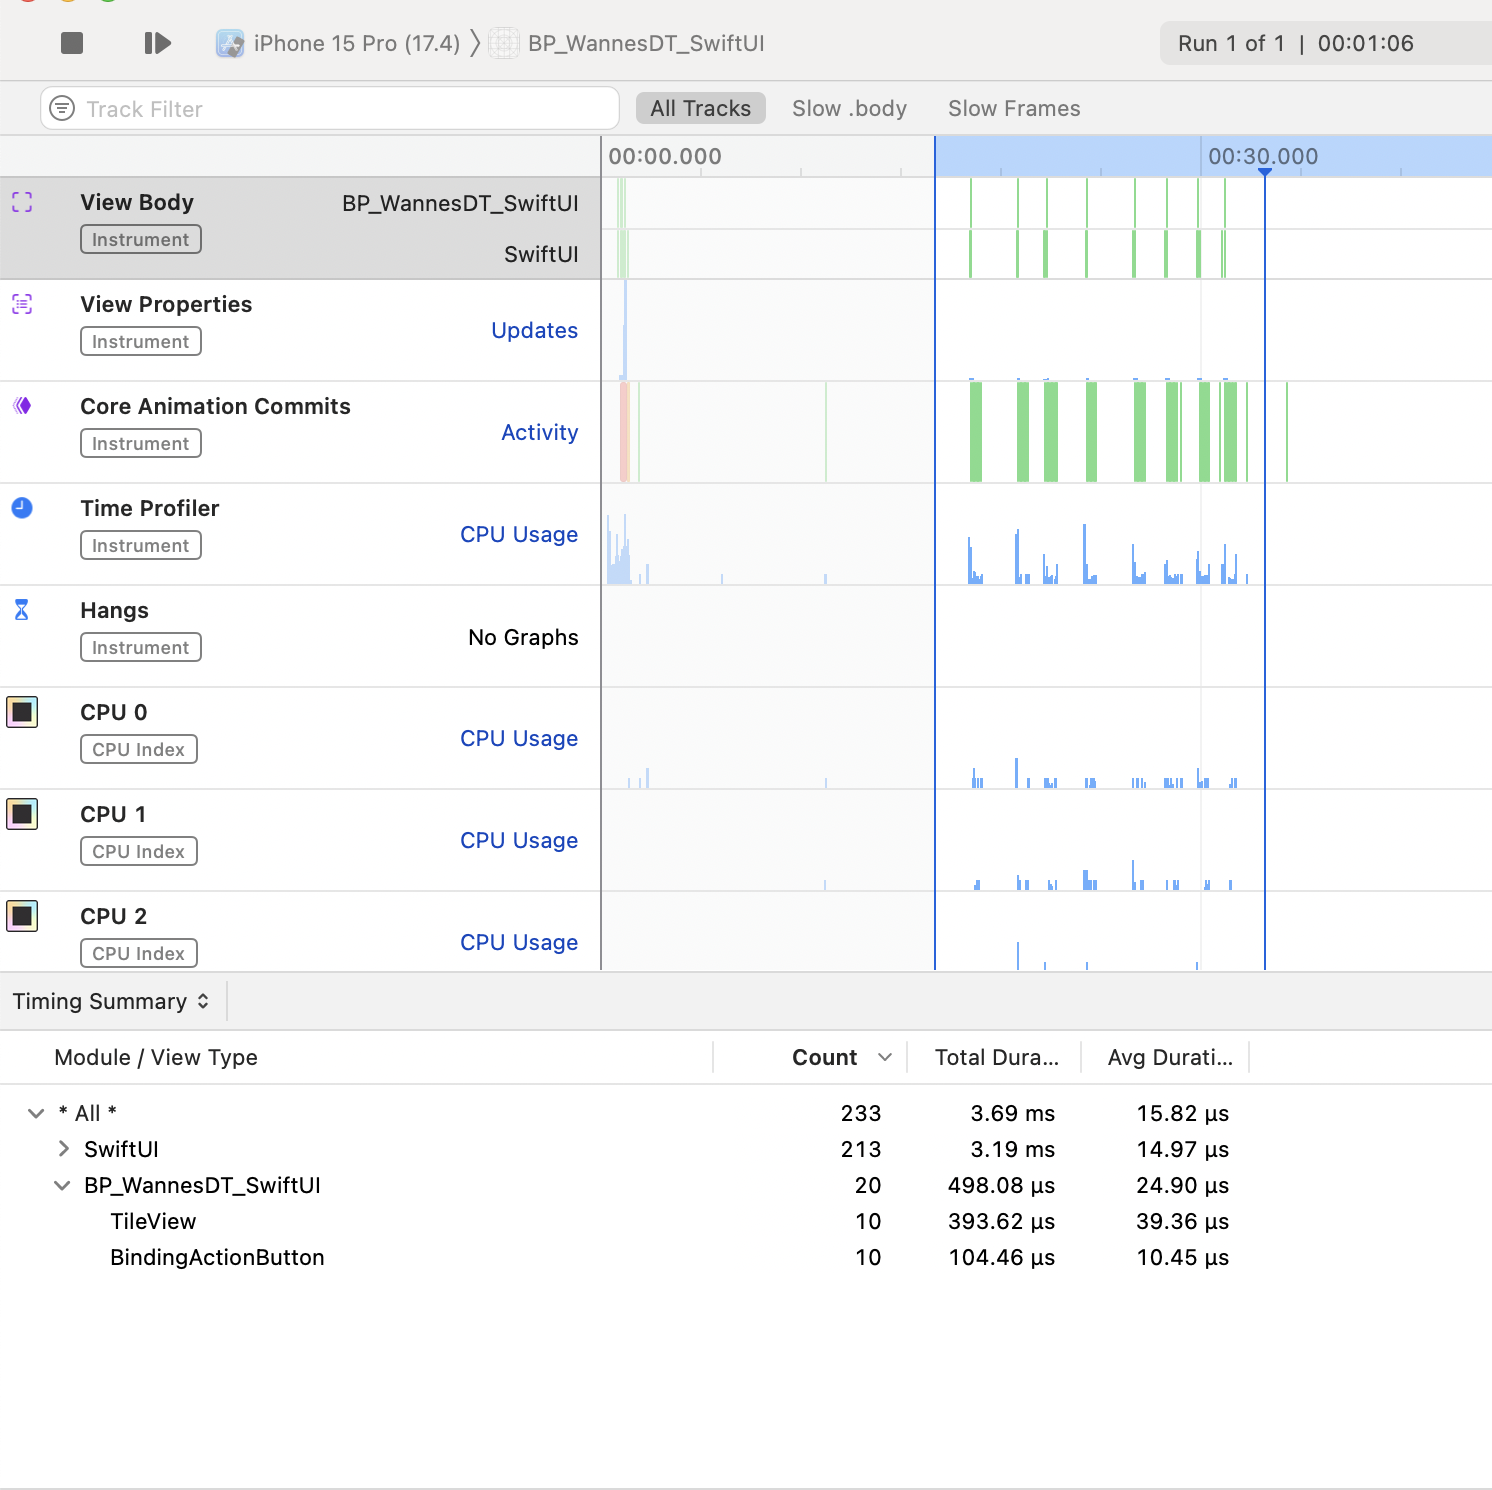
\includegraphics[width=0.7\textwidth]{bptest1_insubview/BindingButtonPressViewRefreshesAndTime} 
    \caption{test2: Aantal keren dat de view refreshed en gemiddelde duratie bij het meervoudig toewijzigen van een binding}
    \label{fig:viewRefreshesBinding1}
\end{figure}
\paragraph{Aantal updates van property's}
\begin{figure}[H]
    \centering
    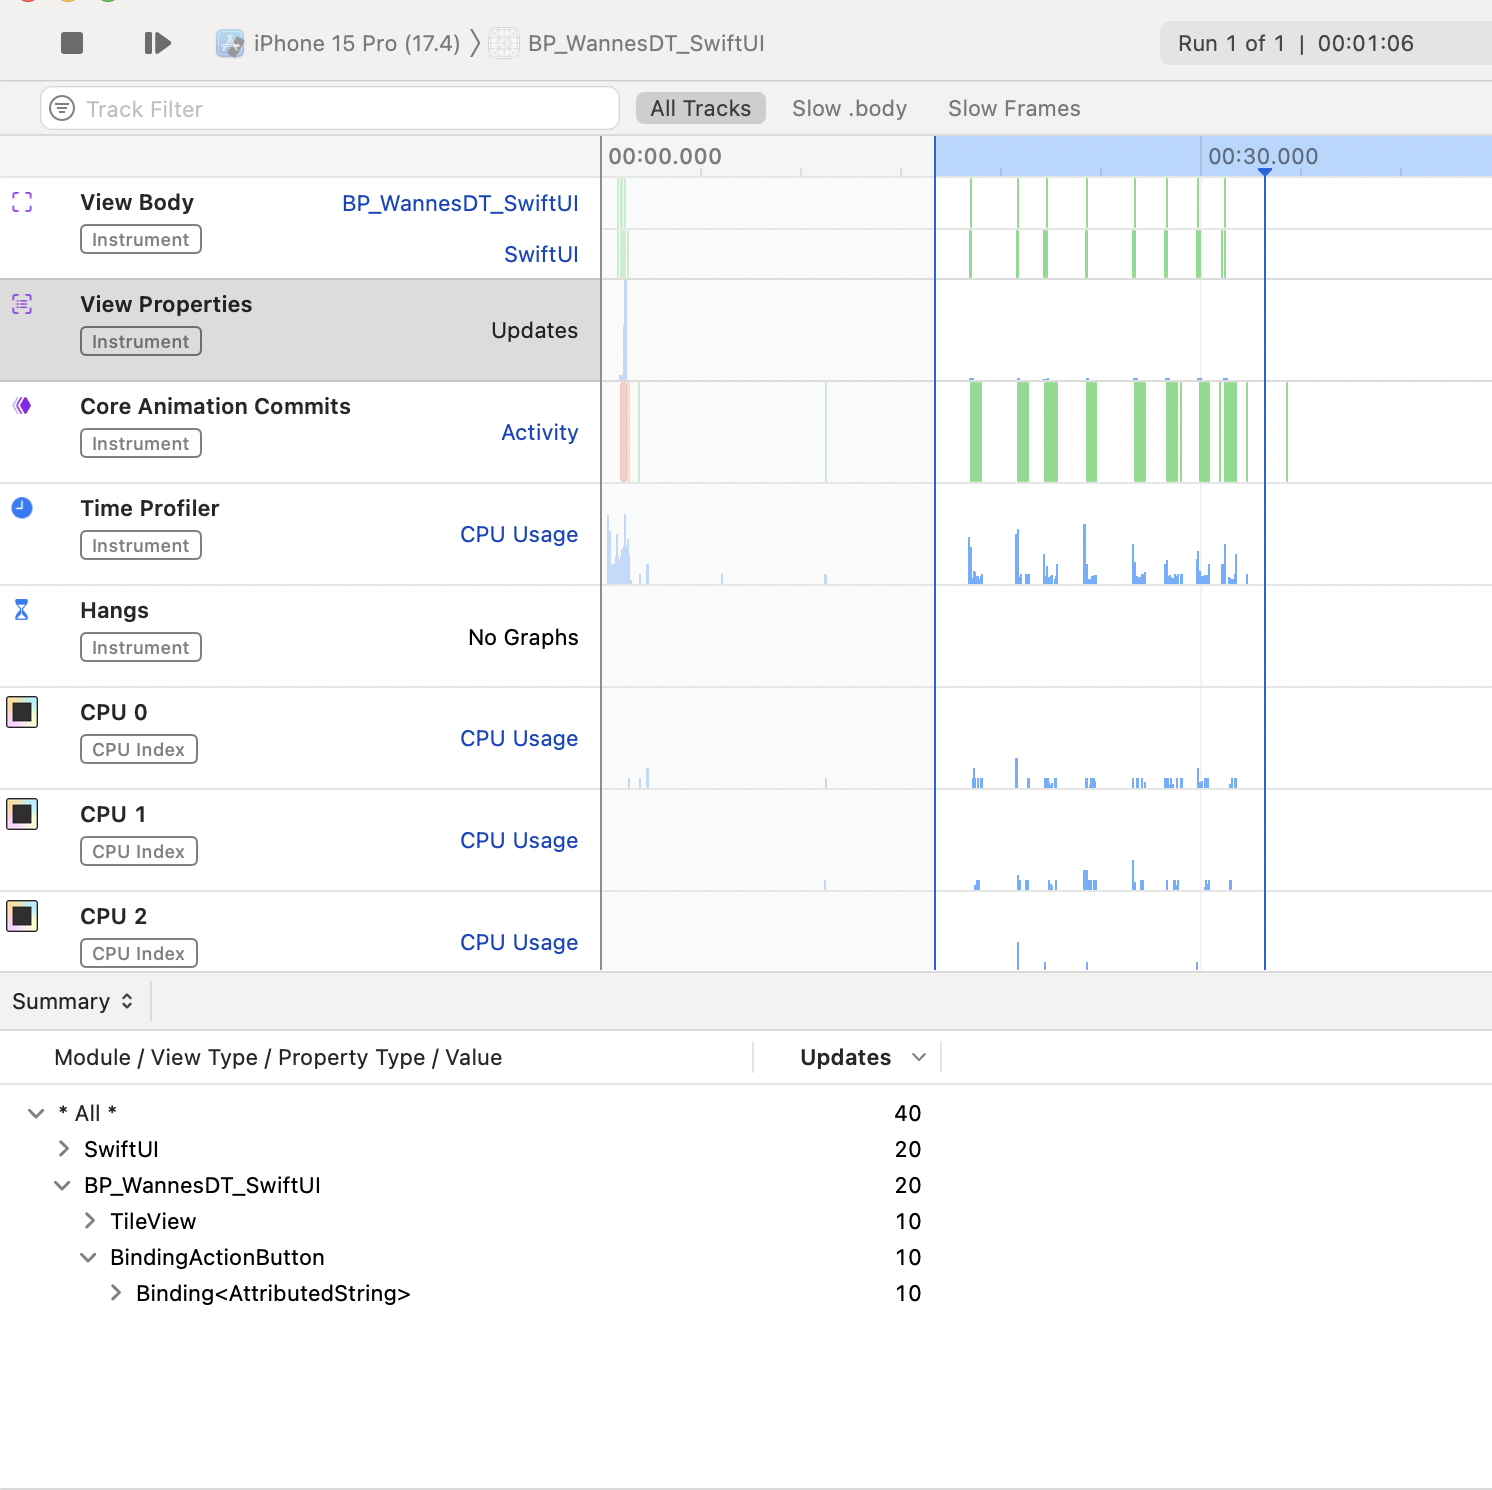
\includegraphics[width=0.7\textwidth]{bptest1_insubview/BindingButtonPressViewPropertyUpdates} 
    \caption{test2: Aantal keren dat de property's updaten bij het meervoudig toewijzigen van een binding}
    \label{fig:propertyUpdatesBinding1}
\end{figure}
\paragraph{Totale tijd gebruikt van de CPU}
\begin{figure}[H]
    \centering
    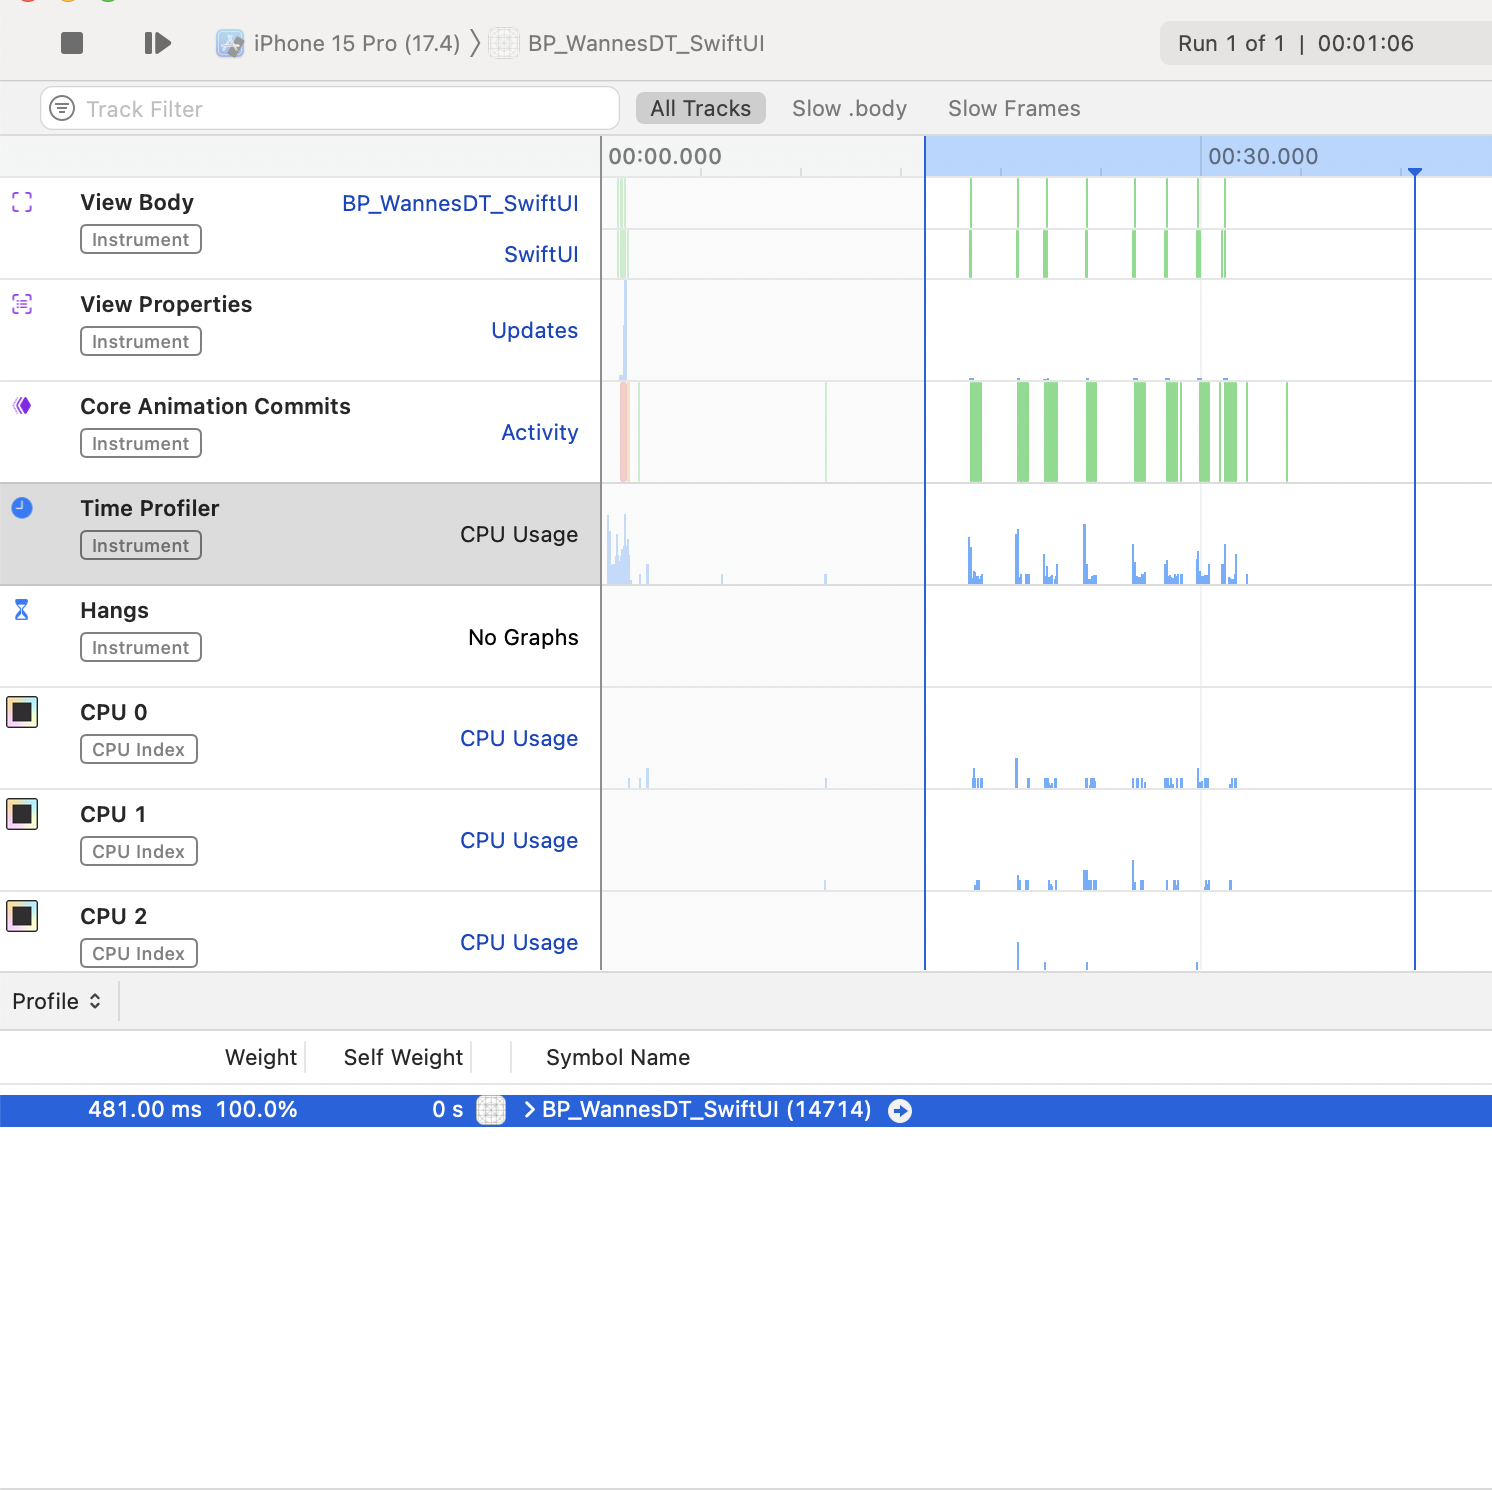
\includegraphics[width=0.7\textwidth]{bptest1_insubview/BindingButtonPressTotalCpuTime} 
    \caption{test2: De totale duratie die gebruikt is van de CPU bij het gebruik van bindings}
    \label{fig:cpuUsageTimeBinding1}
\end{figure}
\paragraph{Last op de CPU}
\begin{figure}[H]
    \centering
    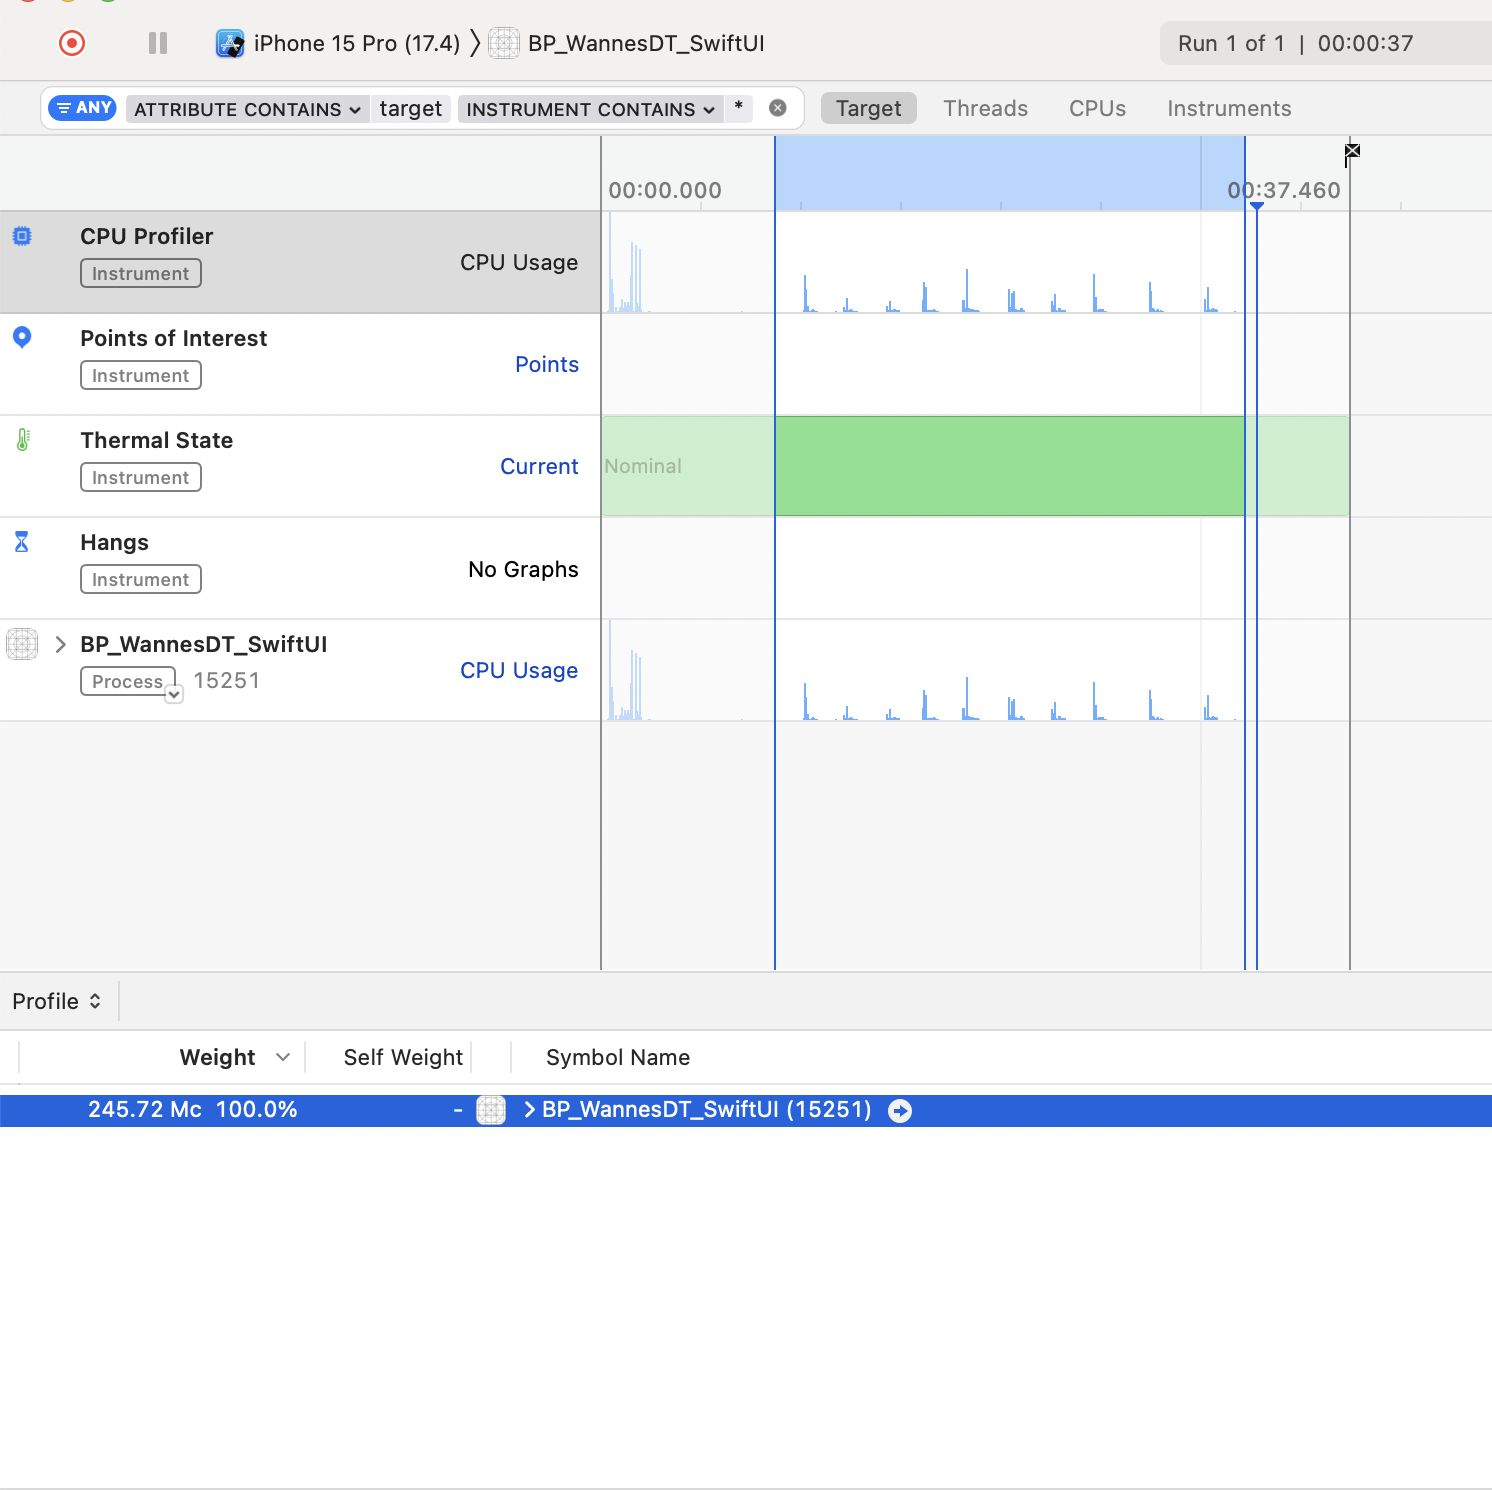
\includegraphics[width=0.7\textwidth]{bptest1_insubview/BindingButtonPressCpuUsage} 
    \caption{test2: De totale last van het opnieuw toewijzen van property's op de cpu bij het gebruik van bindings}
    \label{fig:cpuWeightBinding1}
\end{figure}

% Observable test 1
\subsection{Observable}
\paragraph{View ververs aantal en ververs tijd}
\begin{figure}[H]
    \centering
    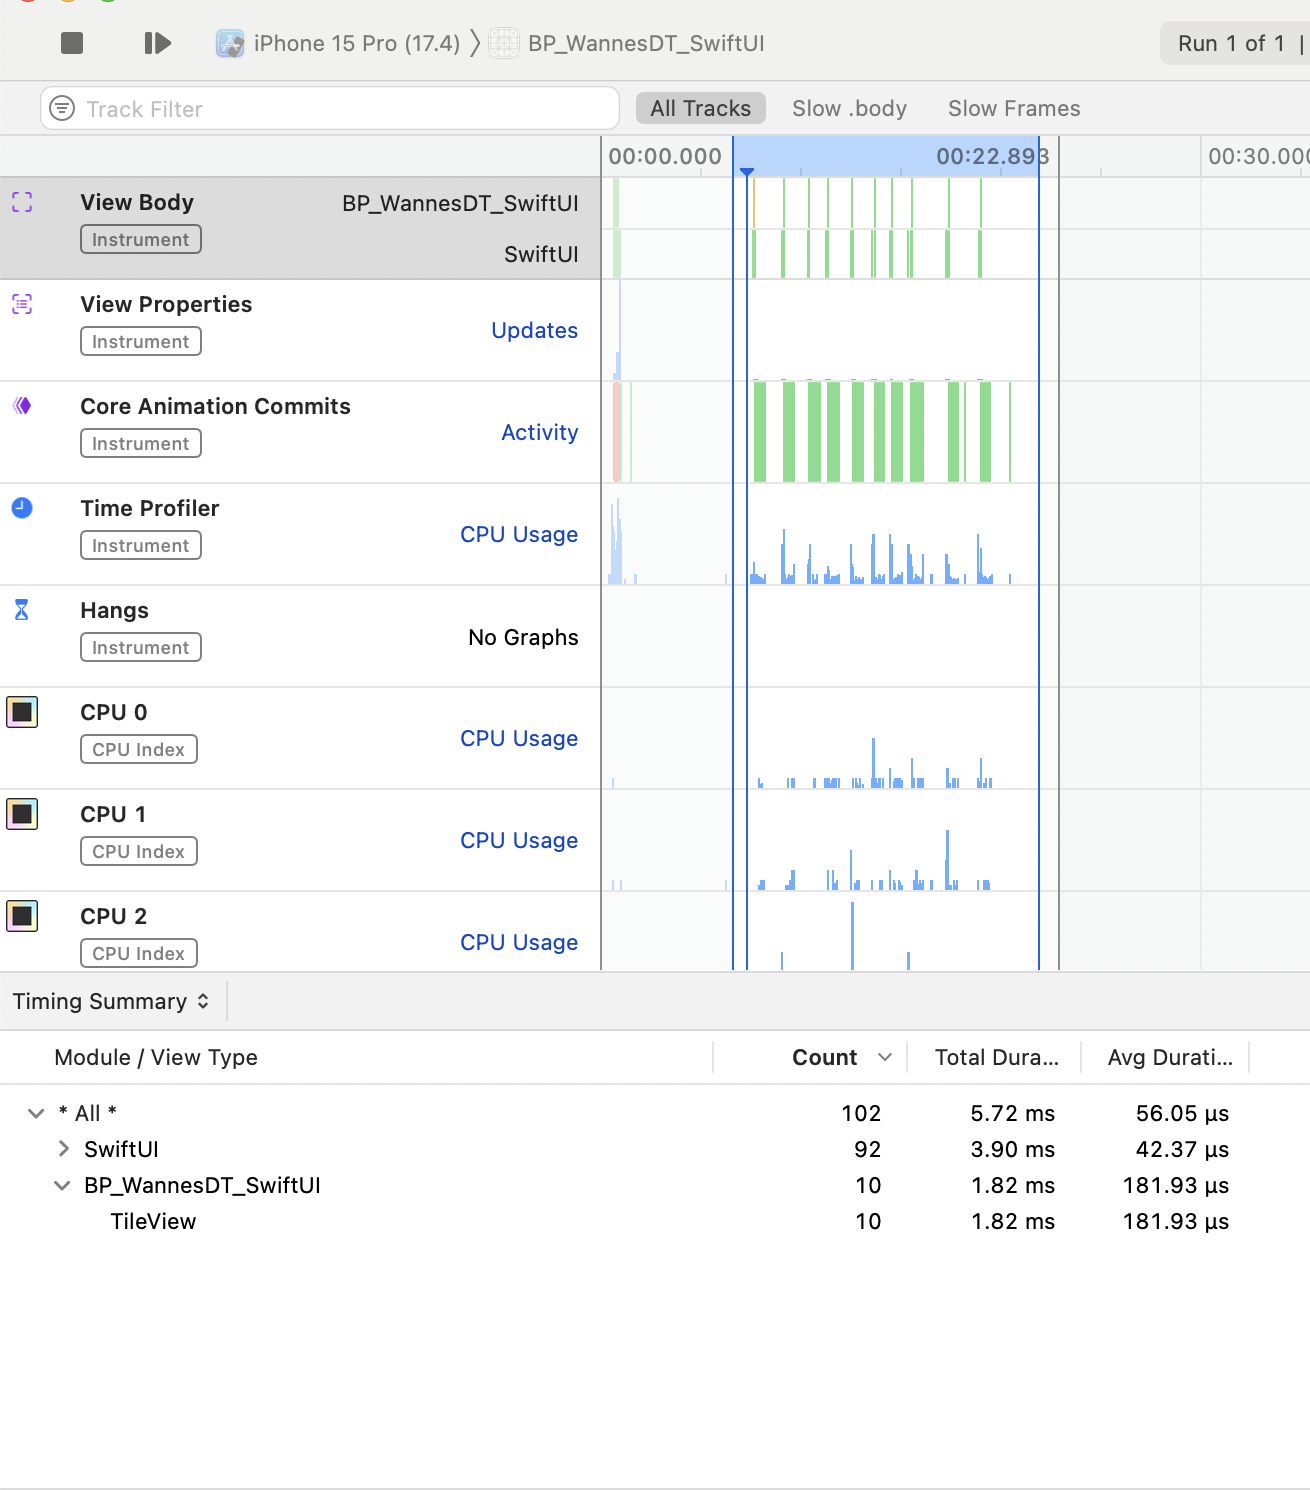
\includegraphics[width=0.7\textwidth]{bptest1_insubview/ObservableButtonPressViewRefreshesAndTime} 
    \caption{test2: Aantal keren dat de view refreshed en gemiddelde duratie bij het meervoudig toewijzigen van een Observable}
    \label{fig:viewRefreshesObservable1}
\end{figure}
\paragraph{Aantal updates van property's}
\begin{figure}[H]
    \centering
    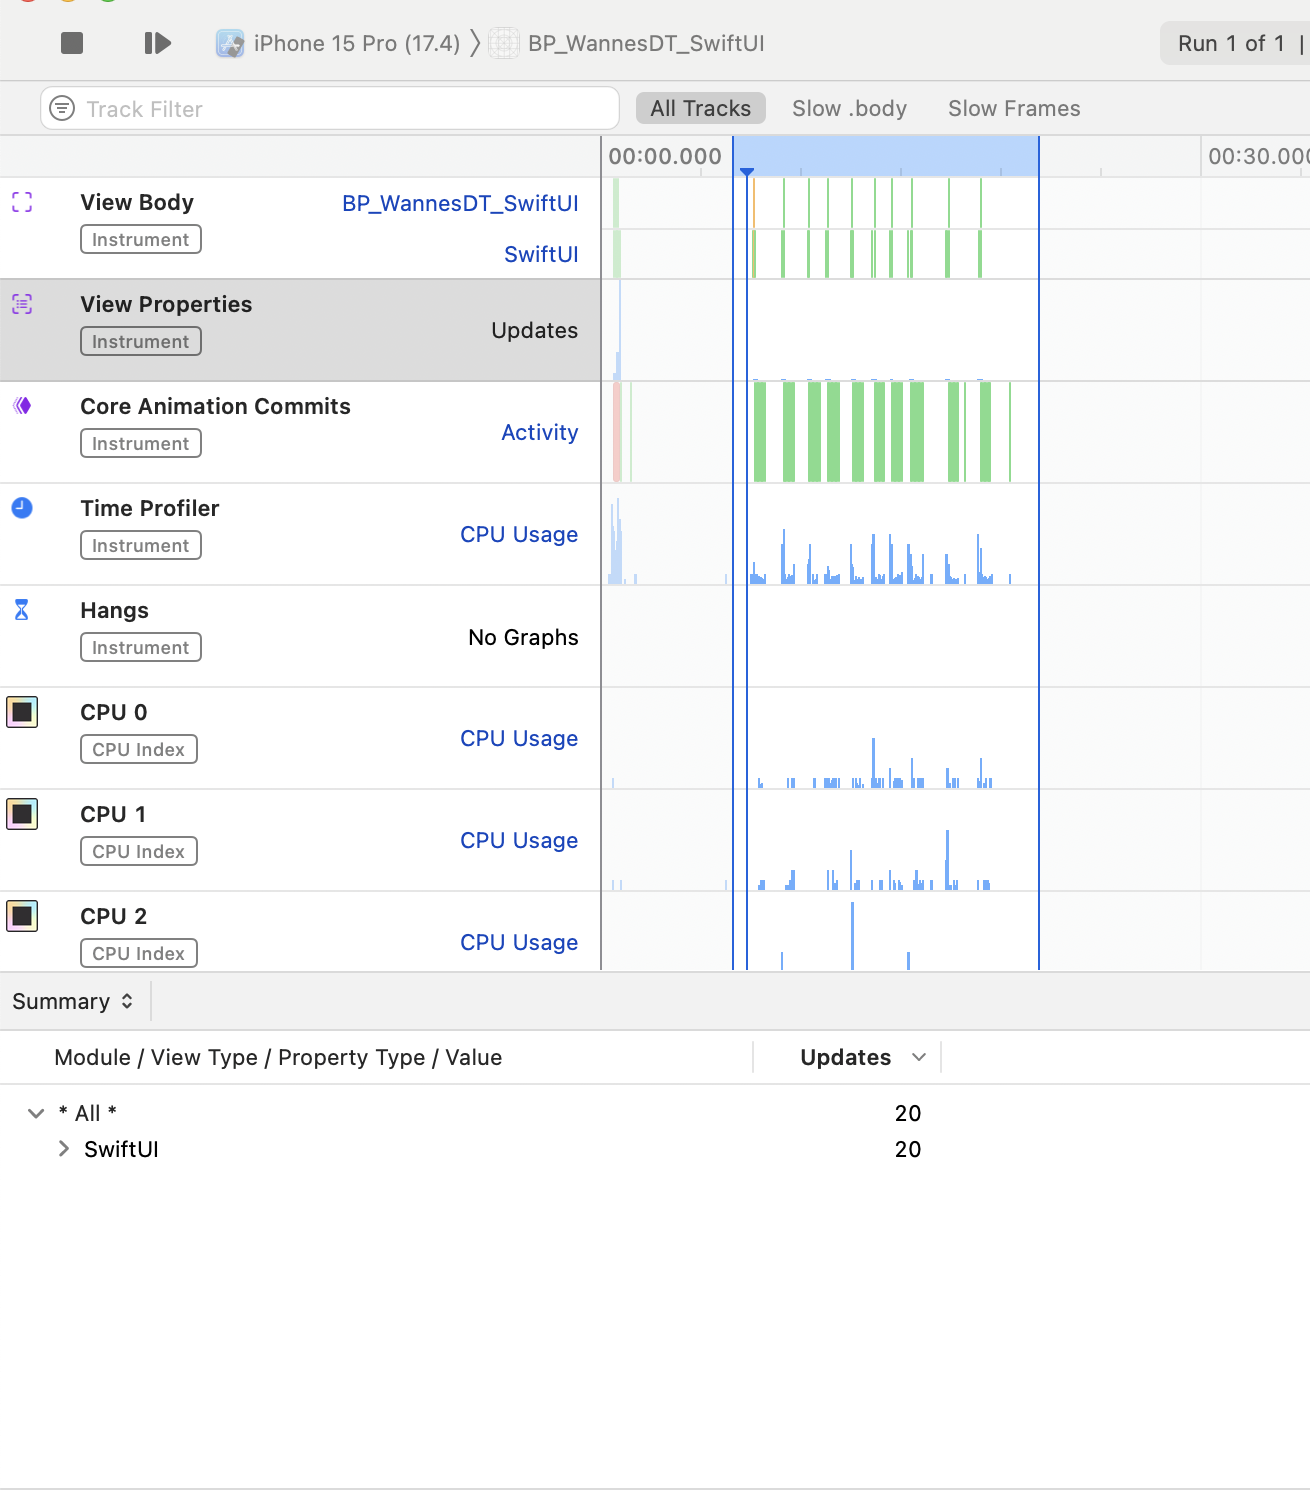
\includegraphics[width=0.7\textwidth]{bptest1_insubview/ObservableButtonPressViewPropertyUpdates} 
    \caption{test2: Aantal keren dat de property's updaten bij het meervoudig toewijzigen van een Observable}
    \label{fig:propertyUpdatesObservable1}
\end{figure}
\paragraph{Totale tijd gebruikt van de CPU}
\begin{figure}[H]
    \centering
    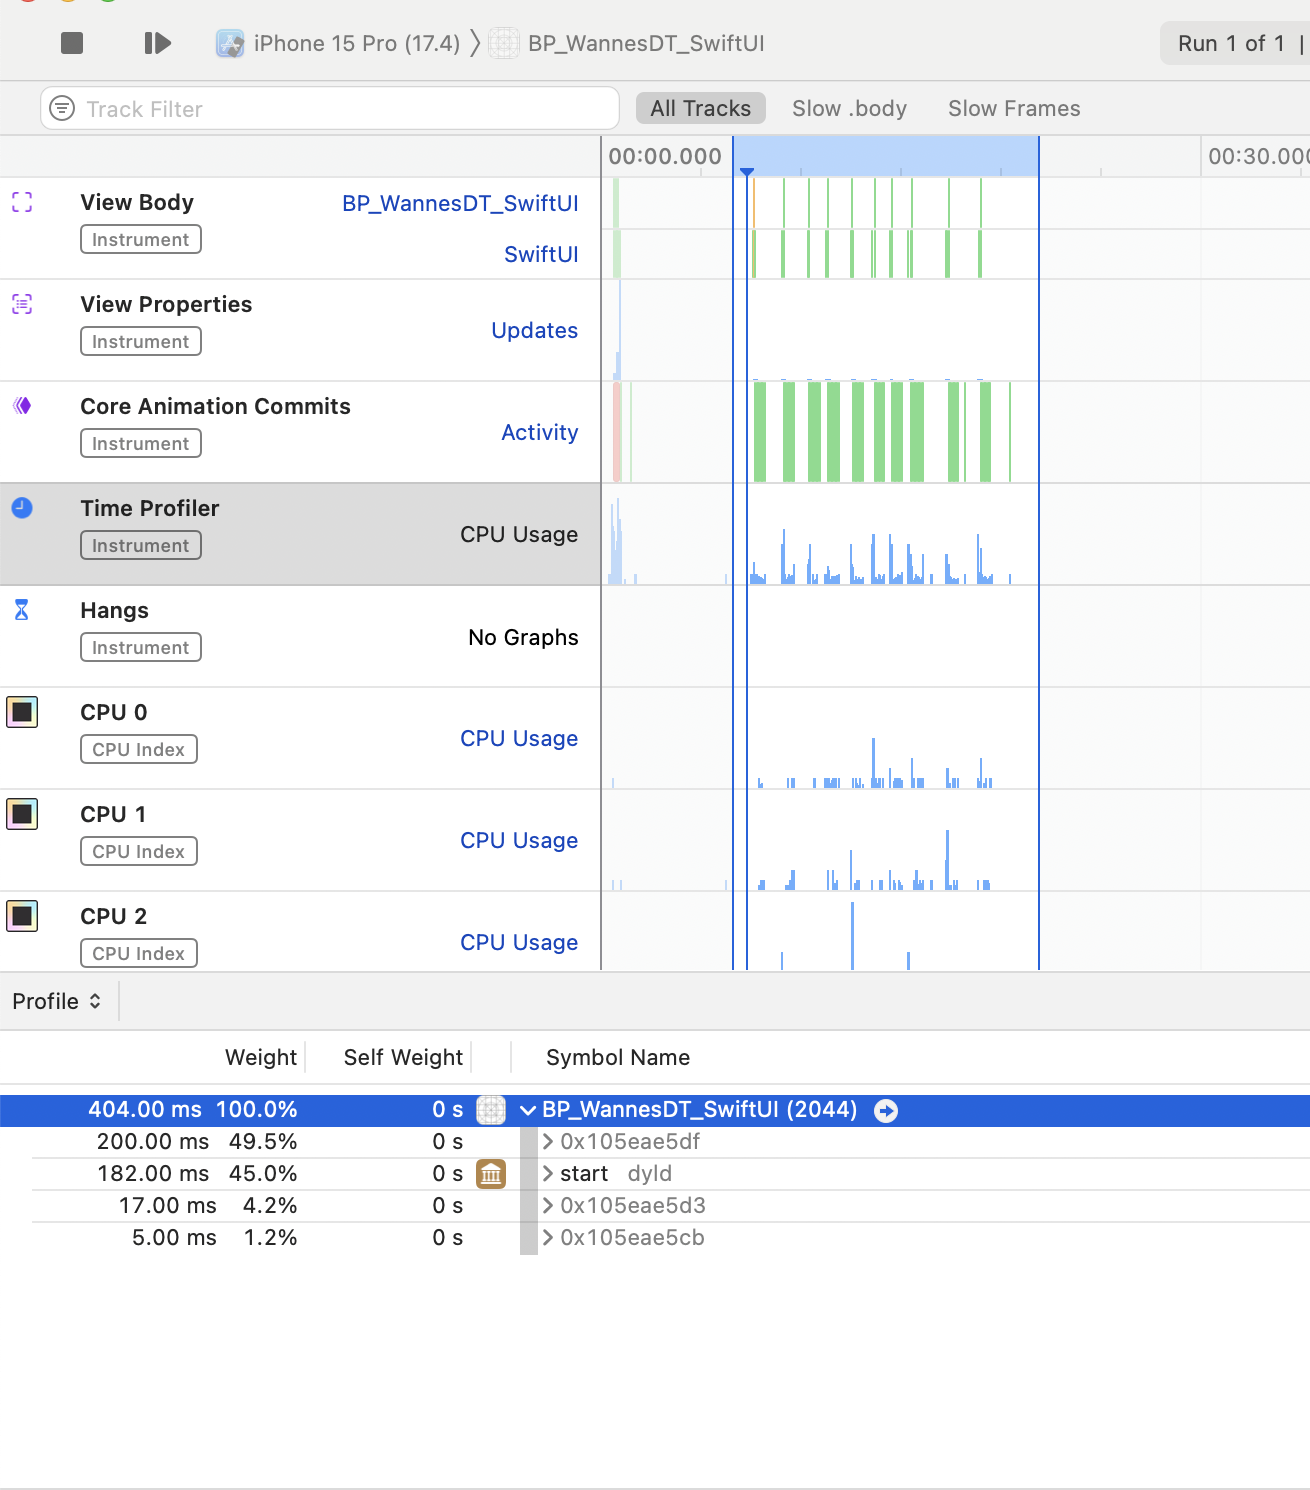
\includegraphics[width=0.7\textwidth]{bptest1_insubview/ObservableButtonPressTotalCpuTime} 
    \caption{test2: De totale duratie die gebruikt is van de CPUbij het gebruik van Observable}
    \label{fig:cpuUsageTimeObservable1}
\end{figure}
\paragraph{Last op de CPU}
\begin{figure}[H]
    \centering
    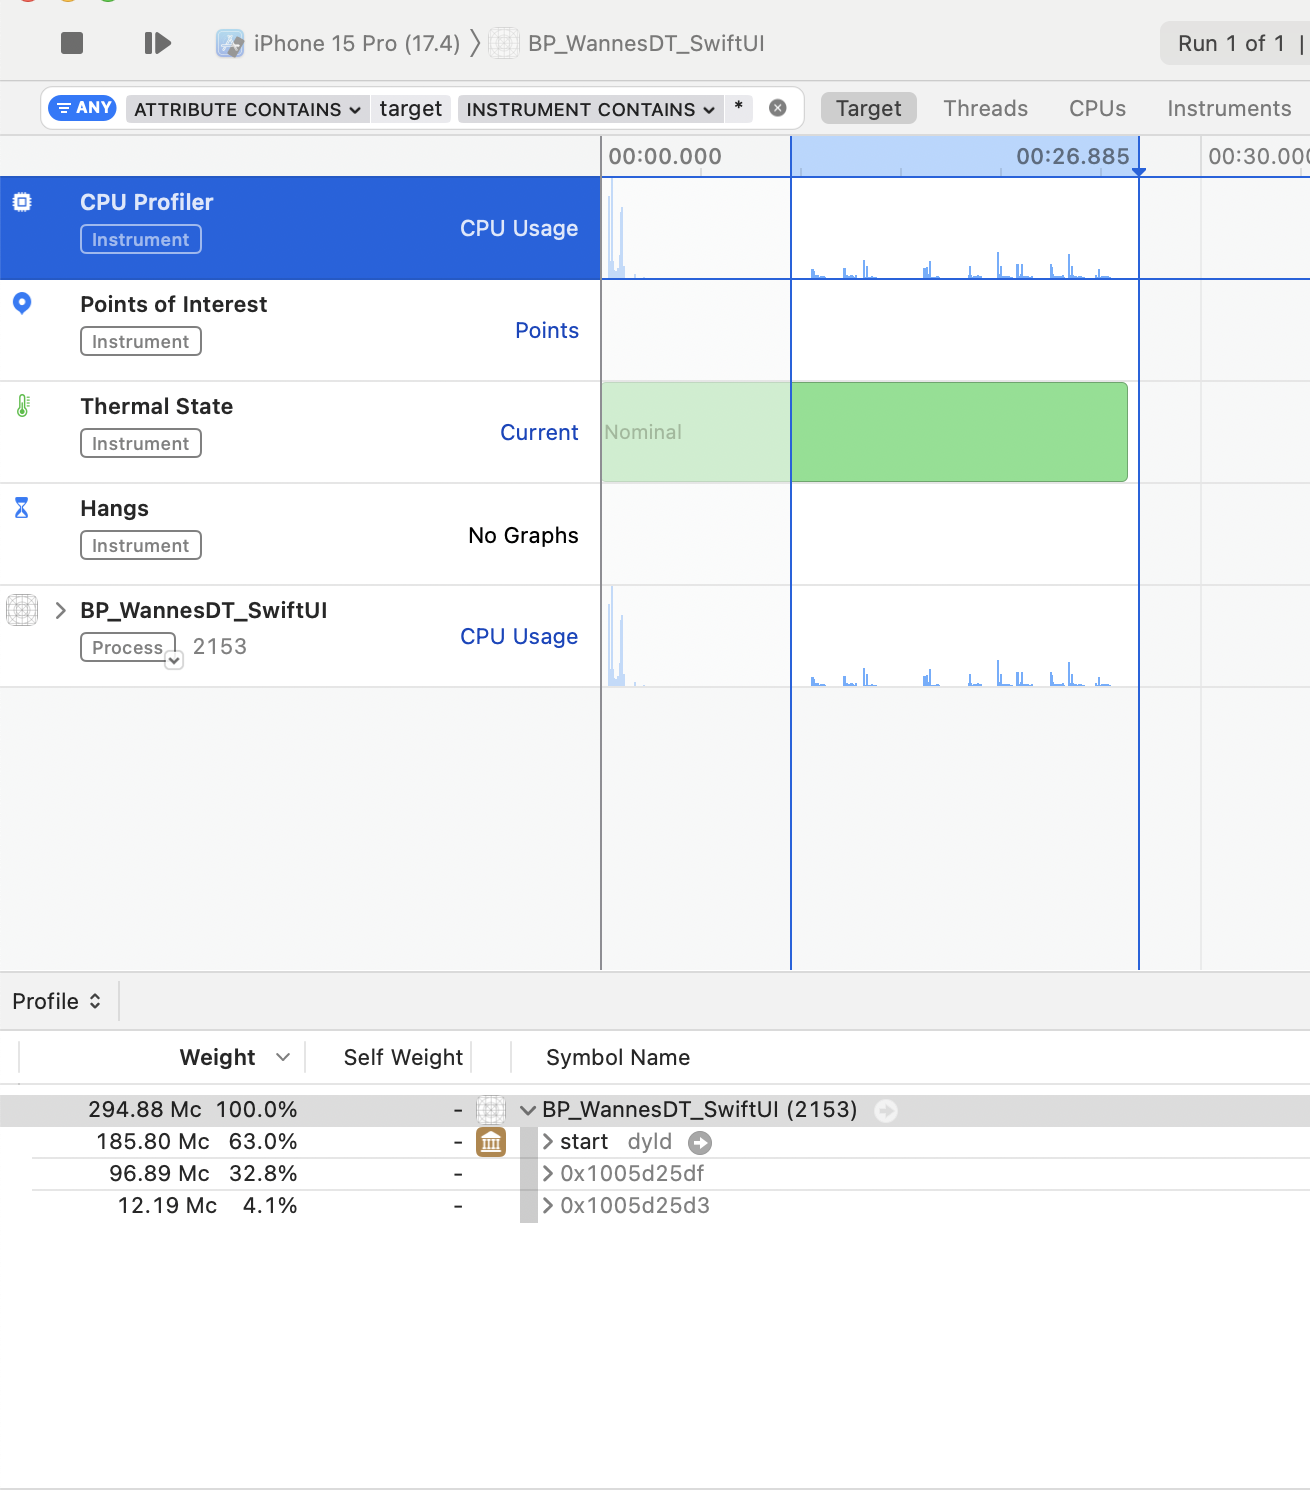
\includegraphics[width=0.7\textwidth]{bptest1_insubview/ObsrvableButtonPressCpuUsage} 
    \caption{test2: De totale last van het opnieuw toewijzen van property's op de cpu bij het gebruik van Observable}
    \label{fig:cpuWeightObservable1}
\end{figure}

\subsection{ObservedObject}
% ObservedObject test 1
\paragraph{View ververs aantal en ververs tijd}
\begin{figure}[H]
    \centering
    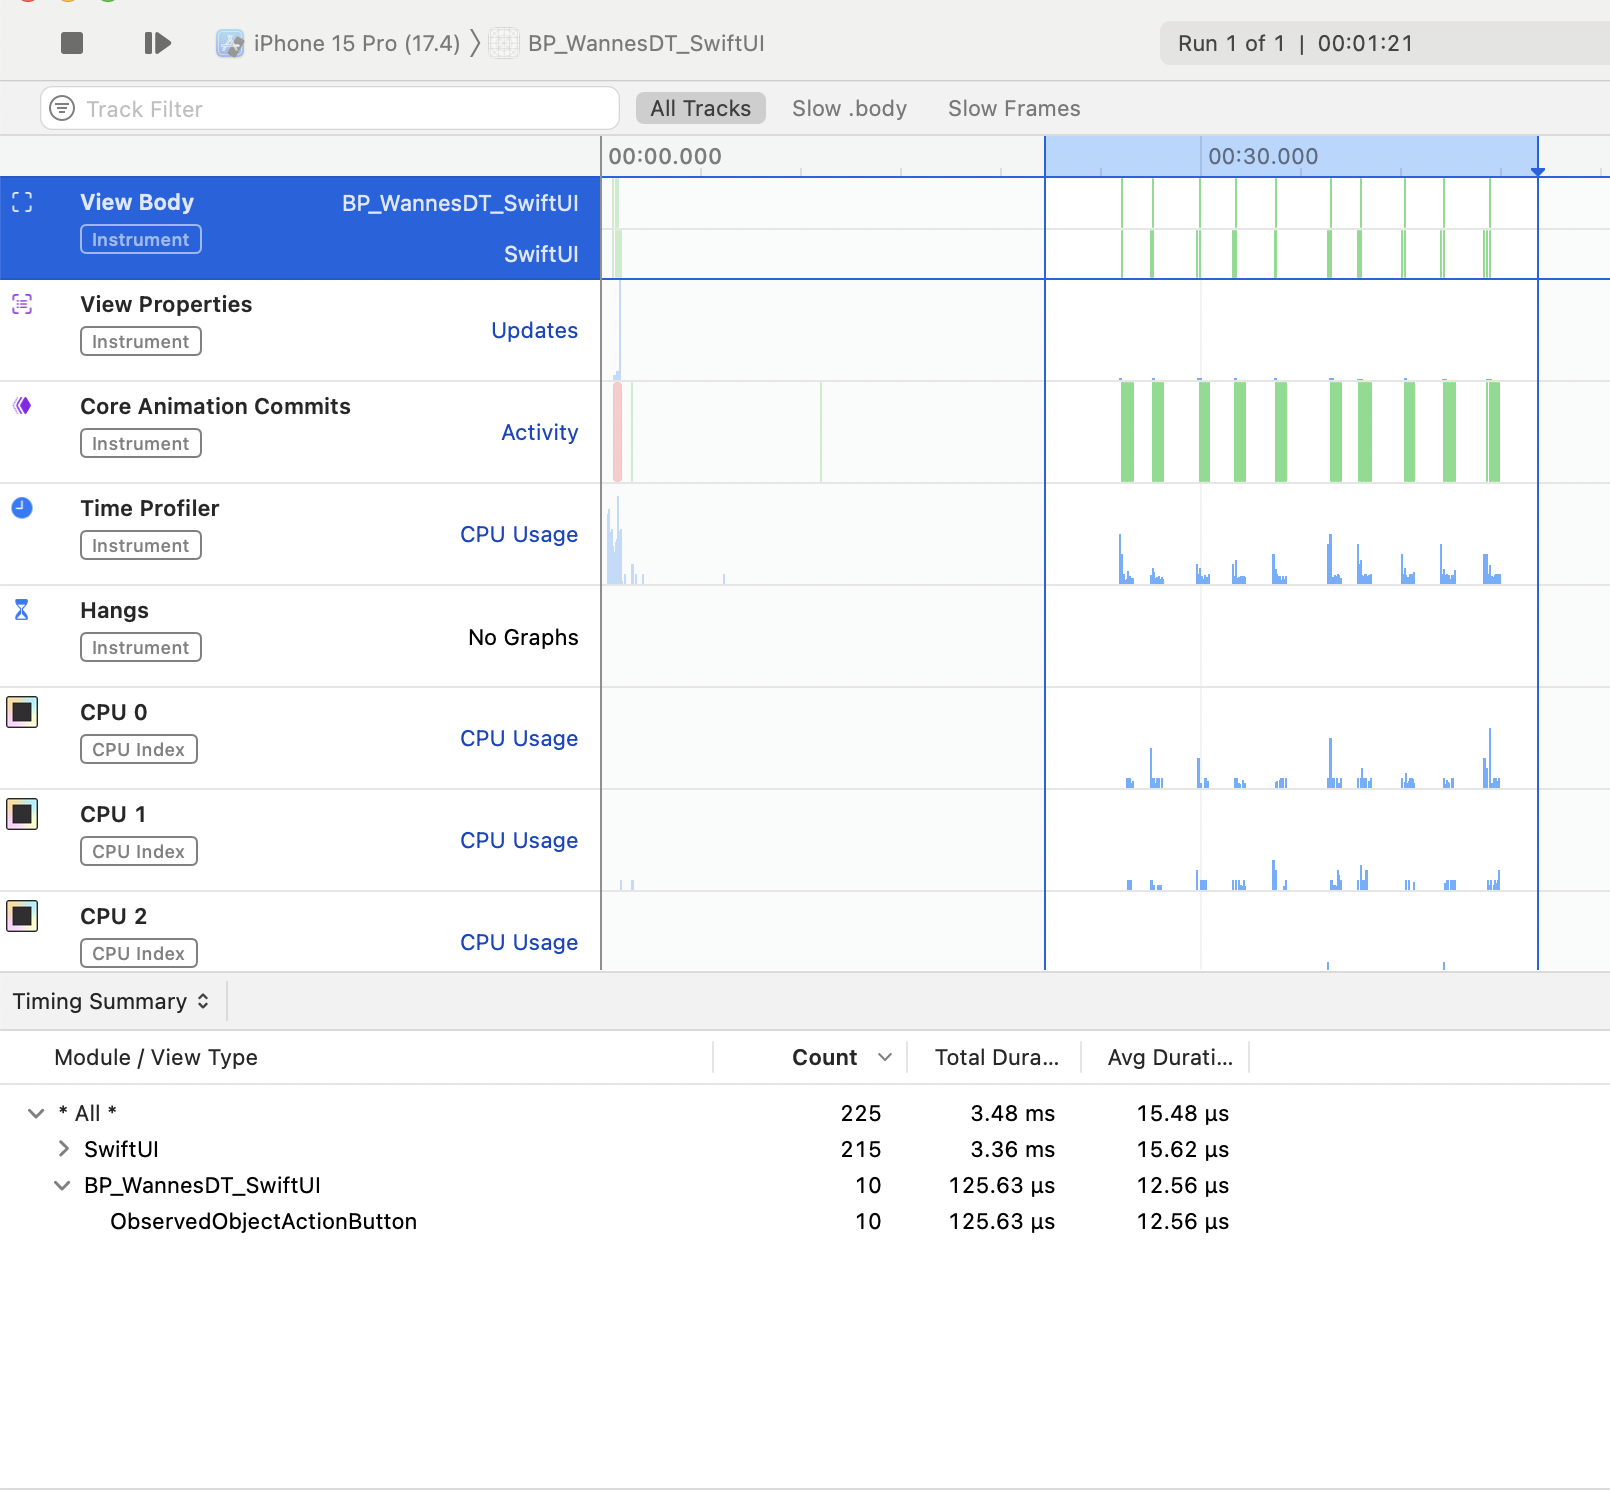
\includegraphics[width=0.7\textwidth]{bptest1_insubview/ObservableObjectButtonPressViewRefreshesAndTime} 
    \caption{test2: Aantal keren dat de view refreshed en gemiddelde duratie bij het meervoudig toewijzigen van een ObservedObject}
    \label{fig:viewRefresheObservedObject1}
\end{figure}
\paragraph{Aantal updates van property's}
\begin{figure}[H]
    \centering
    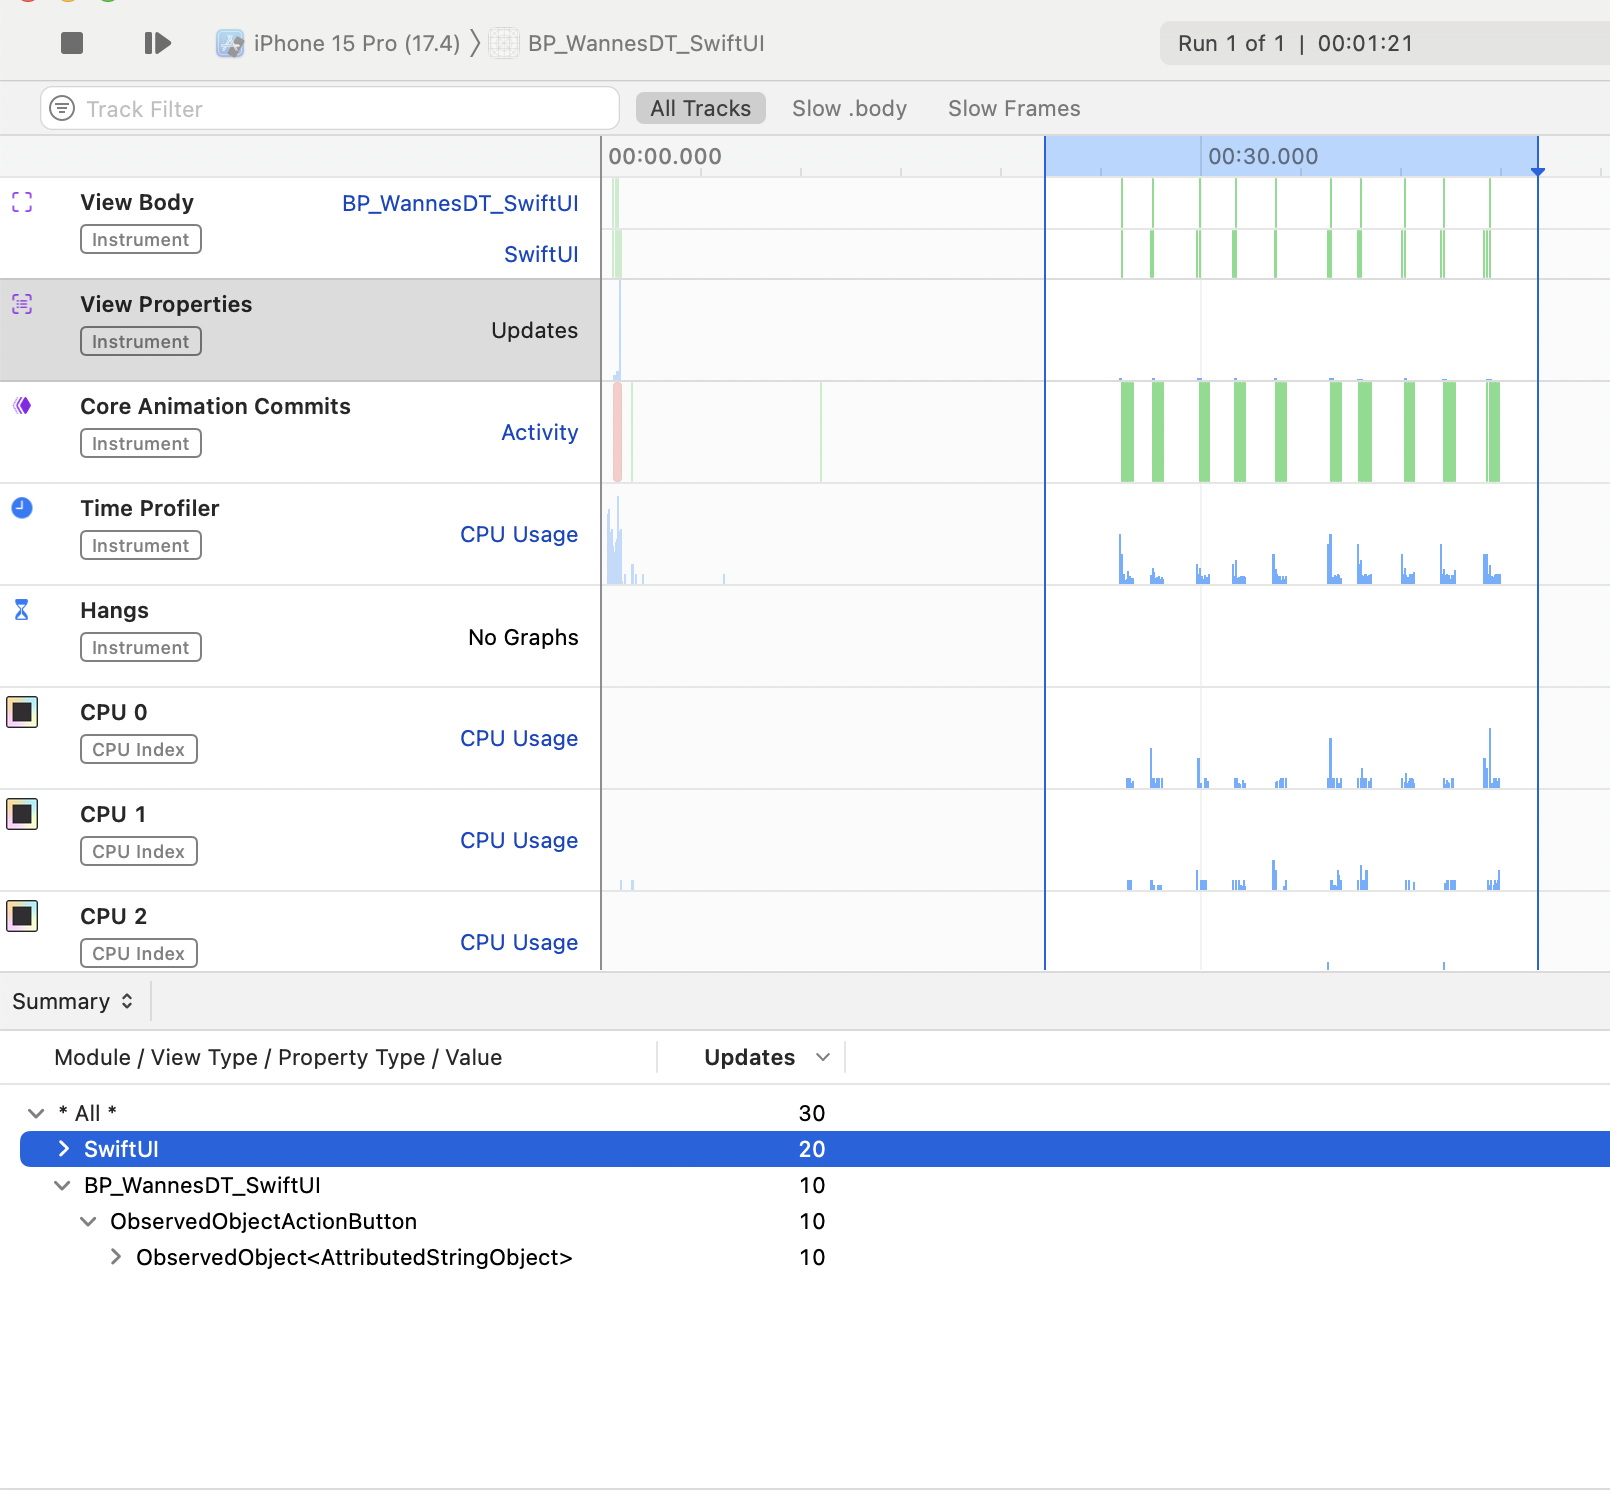
\includegraphics[width=0.7\textwidth]{bptest1_insubview/ObservableObjectButtonPressViewPropertyUpdates} 
    \caption{test2: Aantal keren dat de property's updaten bij het meervoudig toewijzigen van een ObservedObject}
    \label{fig:propertyUpdatesObservedObject1}
\end{figure}
\paragraph{Totale tijd gebruikt van de CPU}
\begin{figure}[H]
    \centering
    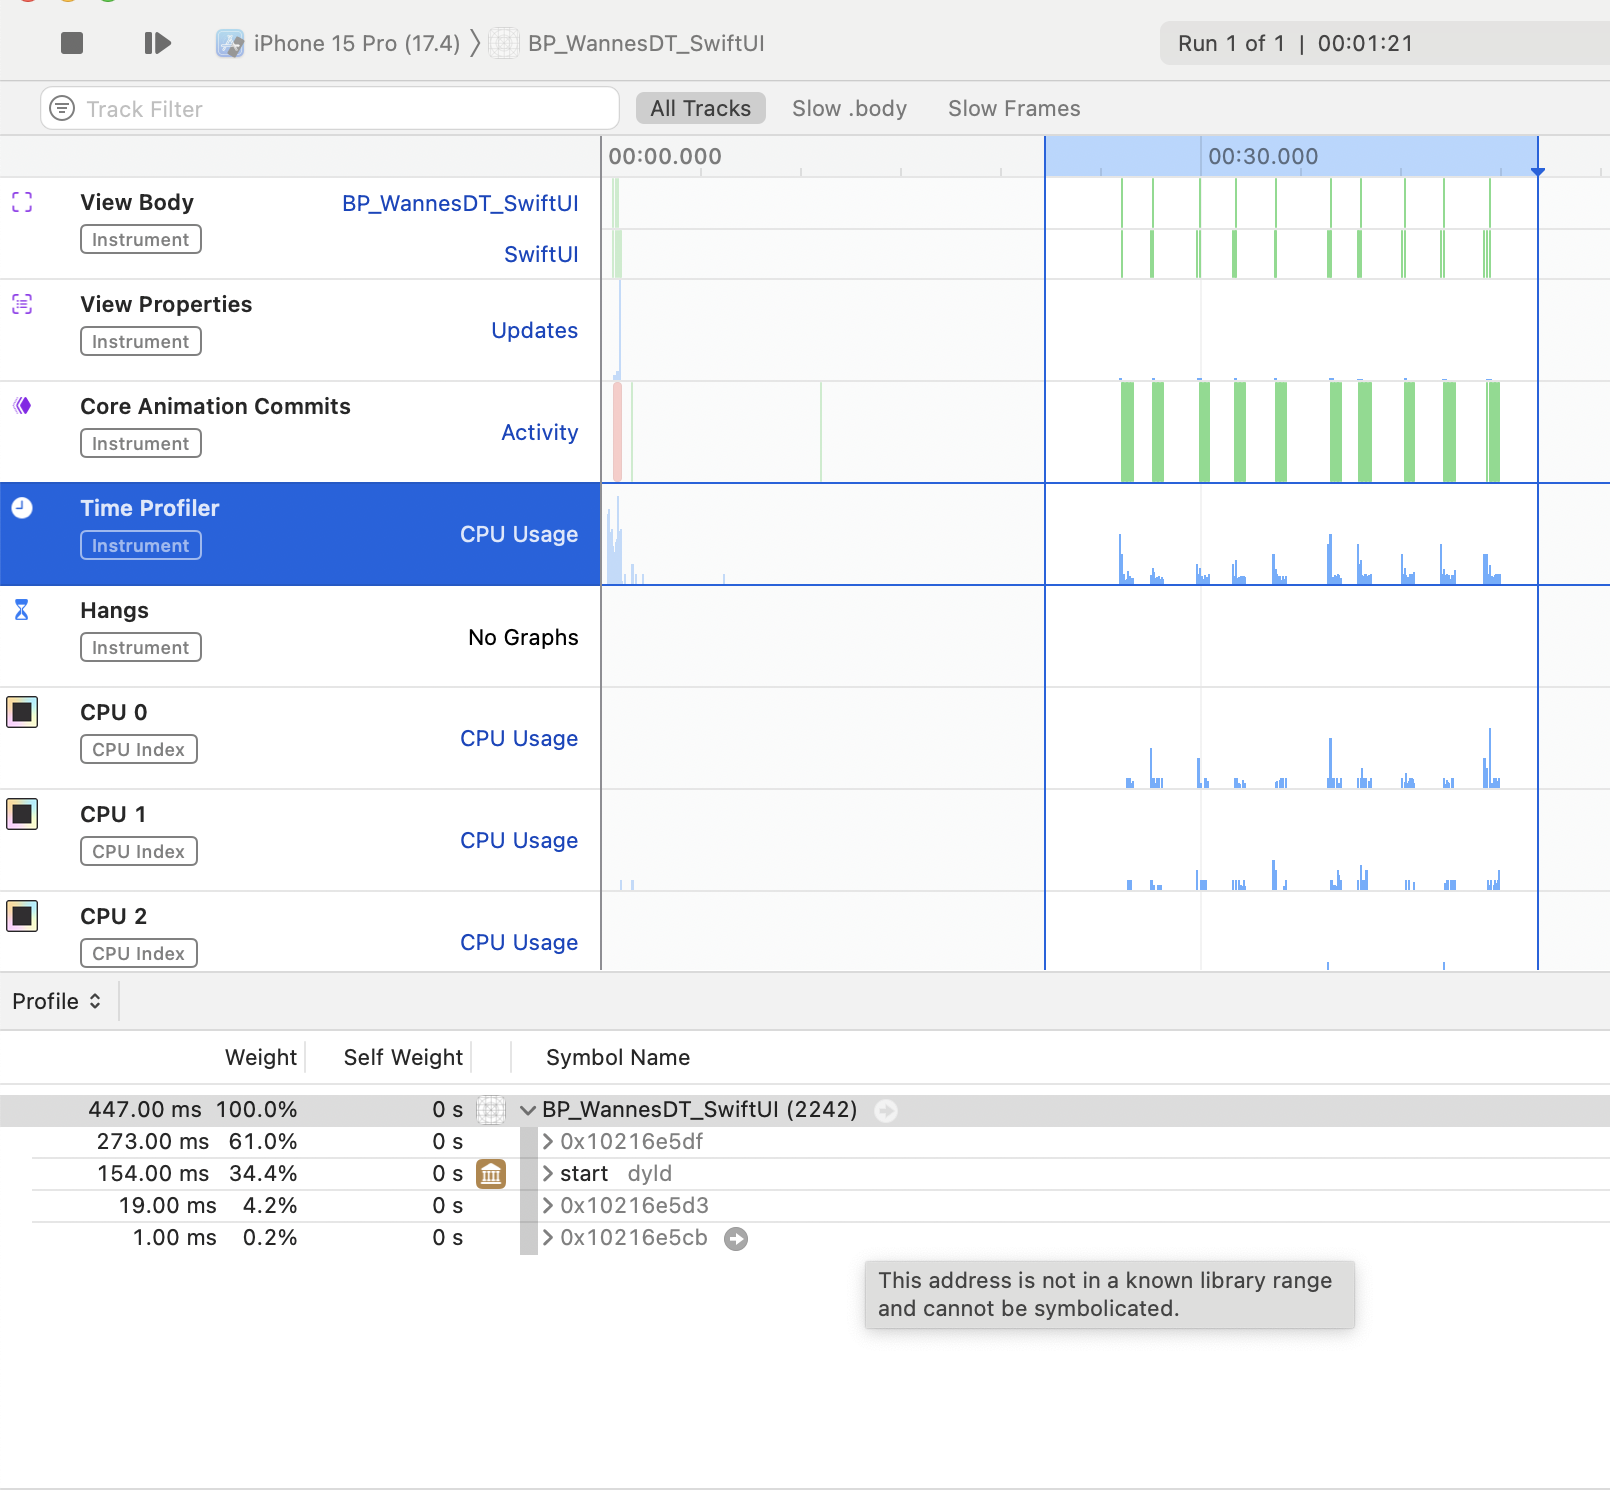
\includegraphics[width=0.7\textwidth]{bptest1_insubview/ObservableObjectButtonPressTotalCpuTime} 
    \caption{test2: De totale duratie die gebruikt is van de CPU bij het gebruik van ObservedObject}
    \label{fig:cpuUsageTimeObservedObject1}
\end{figure}
\paragraph{Last op de CPU}
\begin{figure}[H]
    \centering
    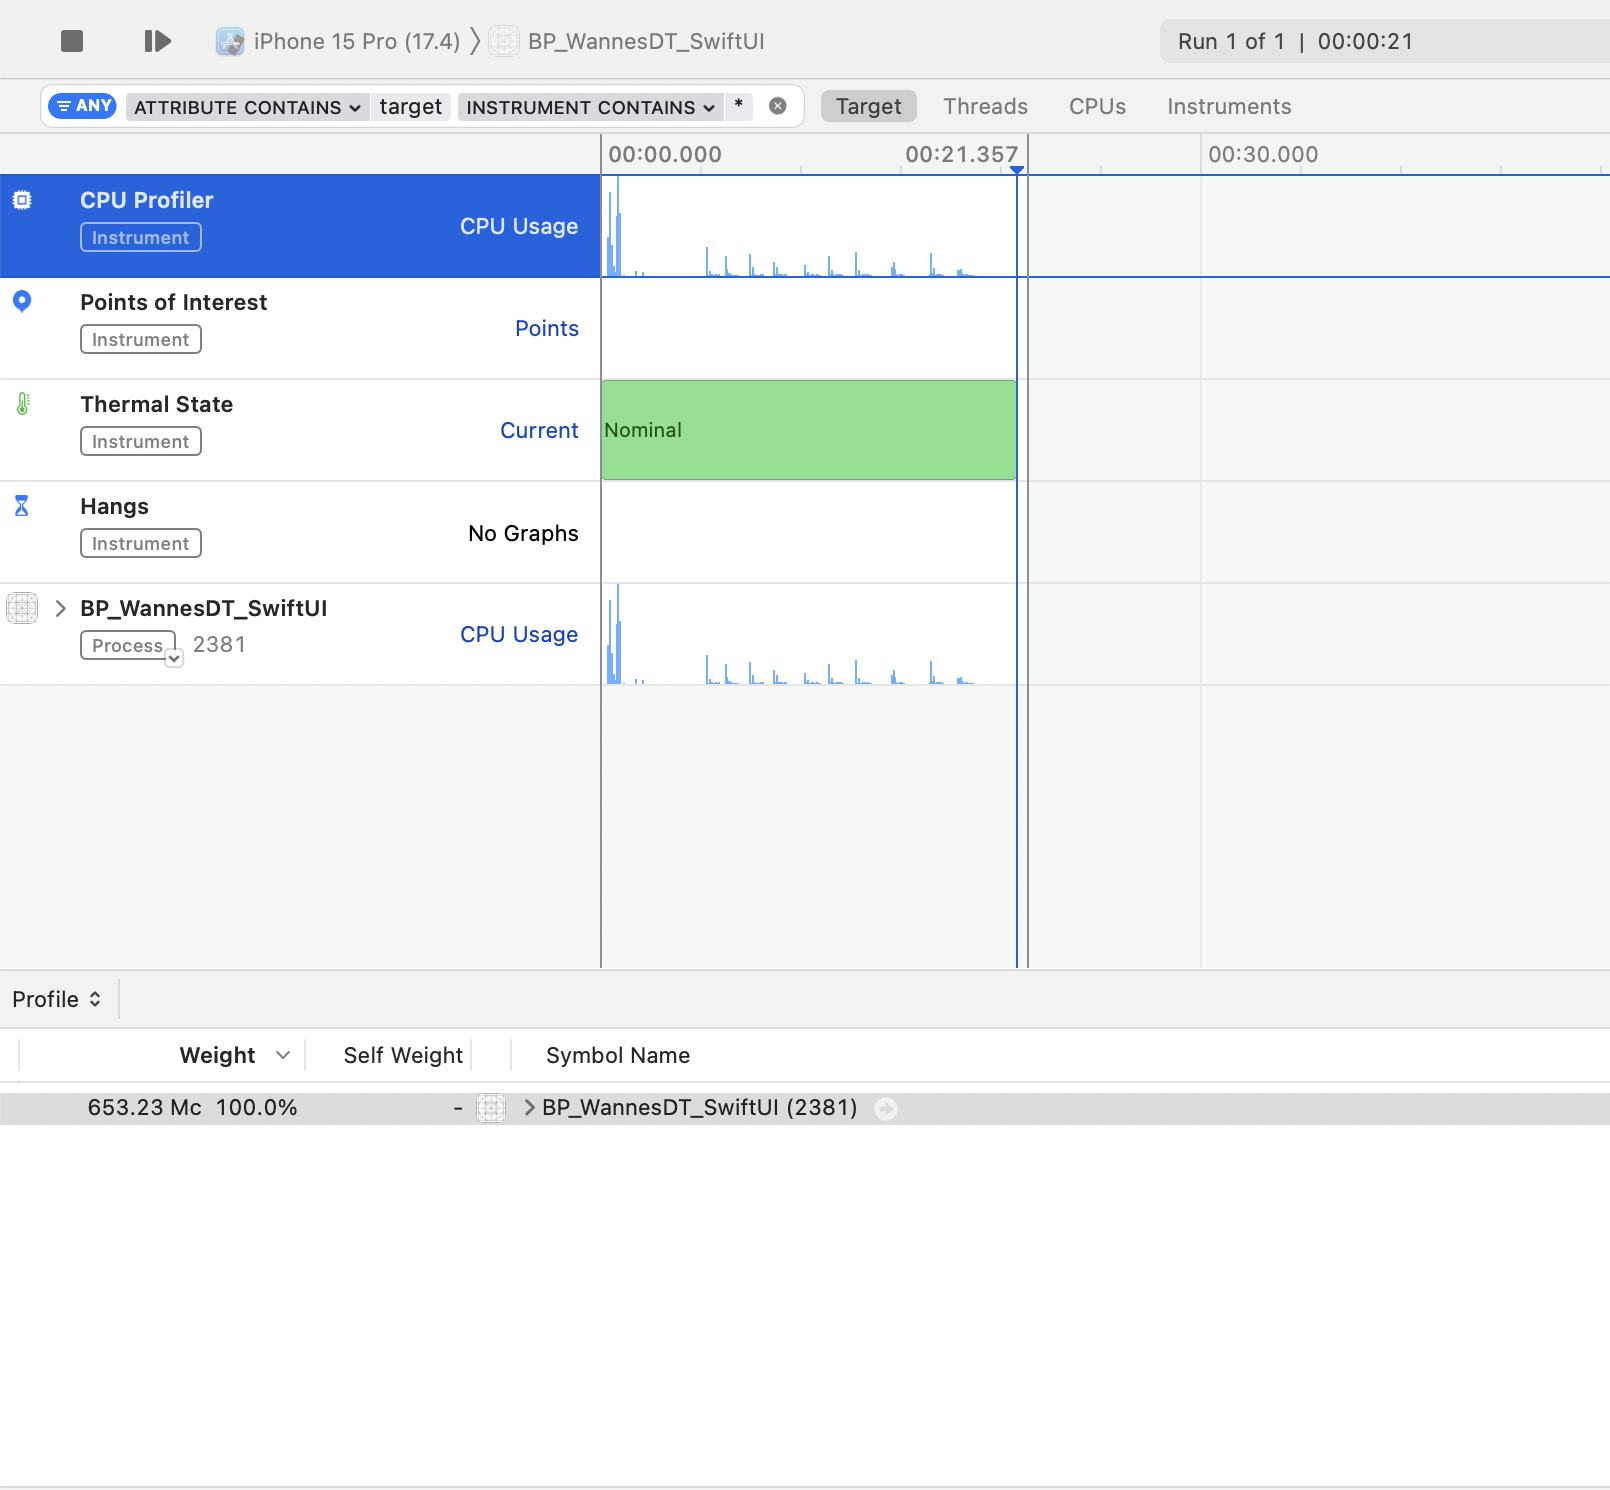
\includegraphics[width=0.7\textwidth]{bptest1_insubview/ObsrvableObjectButtonPressCpuUsage} 
    \caption{test2: De totale last van het opnieuw toewijzen van property's op de cpu bij het gebruik van ObservedObject}
    \label{fig:cpuWeightObservedObject1}
\end{figure}

\subsection{EnvironmentObject}
% EnvironmentObject test 1
\paragraph{View ververs aantal en ververs tijd}
\begin{figure}[H]
    \centering
    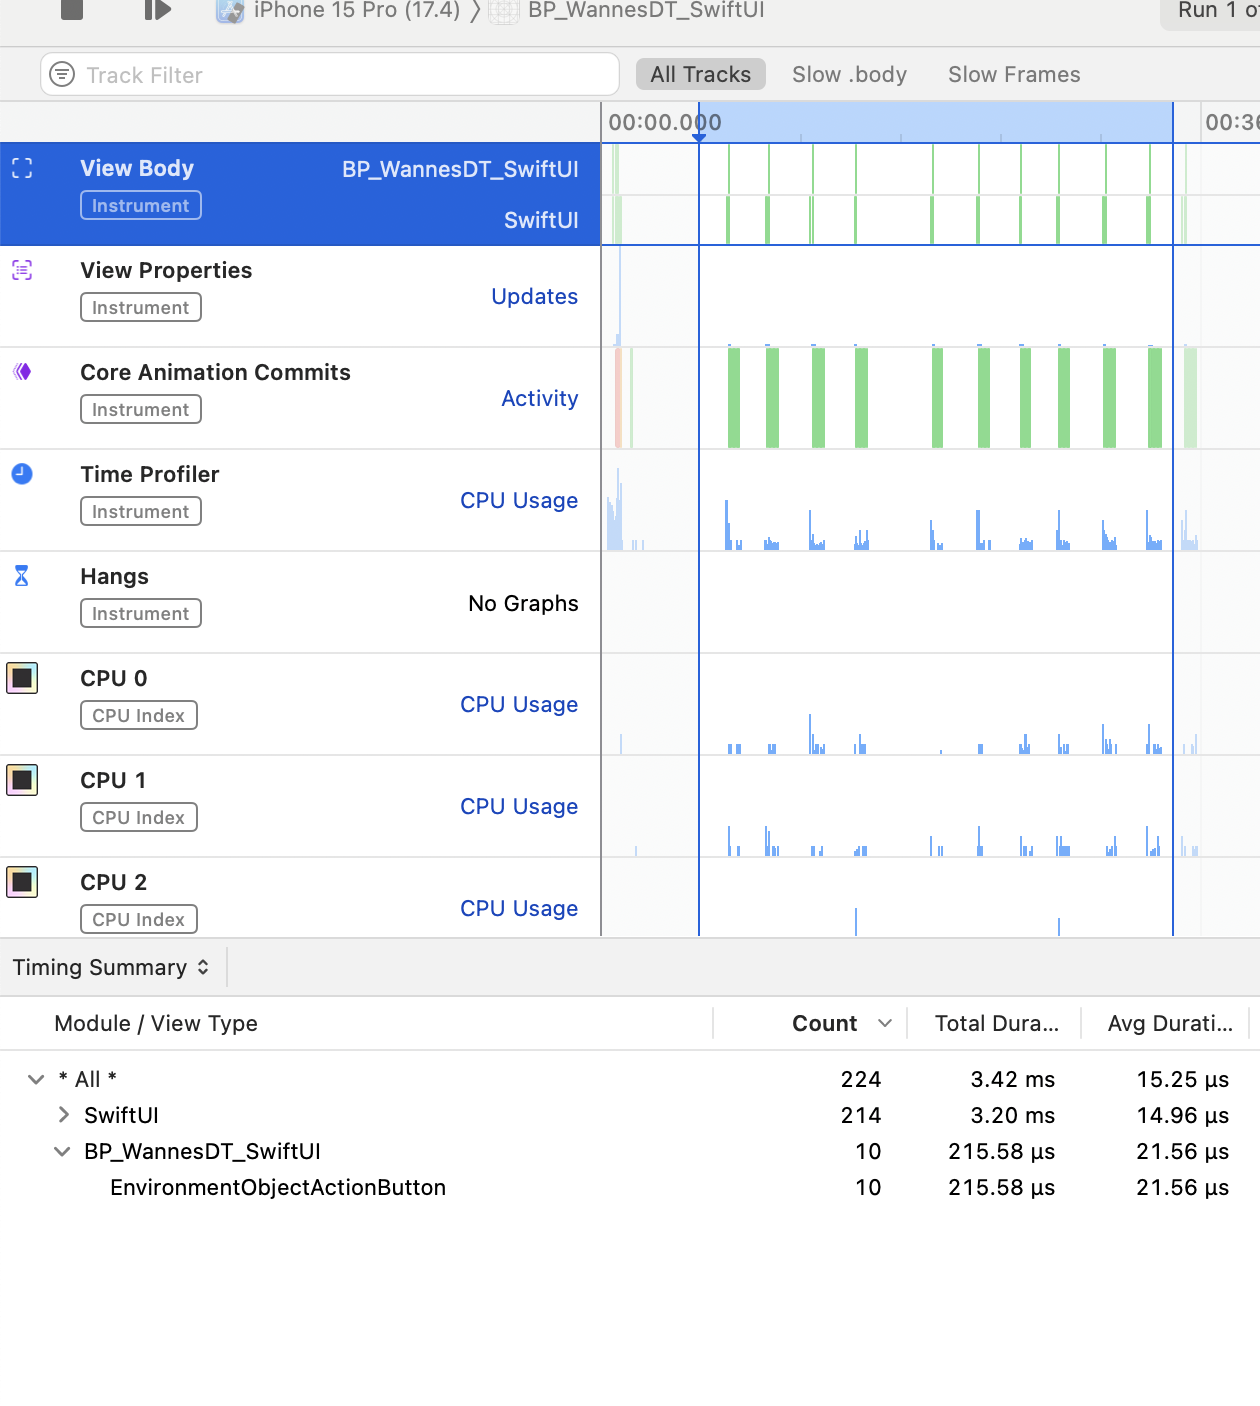
\includegraphics[width=0.7\textwidth]{bptest1_insubview/EnvironmentObjectButtonPressViewRefreshesAndTime} 
    \caption{test2: Aantal keren dat de view refreshed en gemiddelde duratie bij het meervoudig toewijzigen van een EnvironmentObject}
    \label{fig:viewRefresheEnvironmentObject1}
\end{figure}
\paragraph{Aantal updates van property's}
\begin{figure}[H]
    \centering
    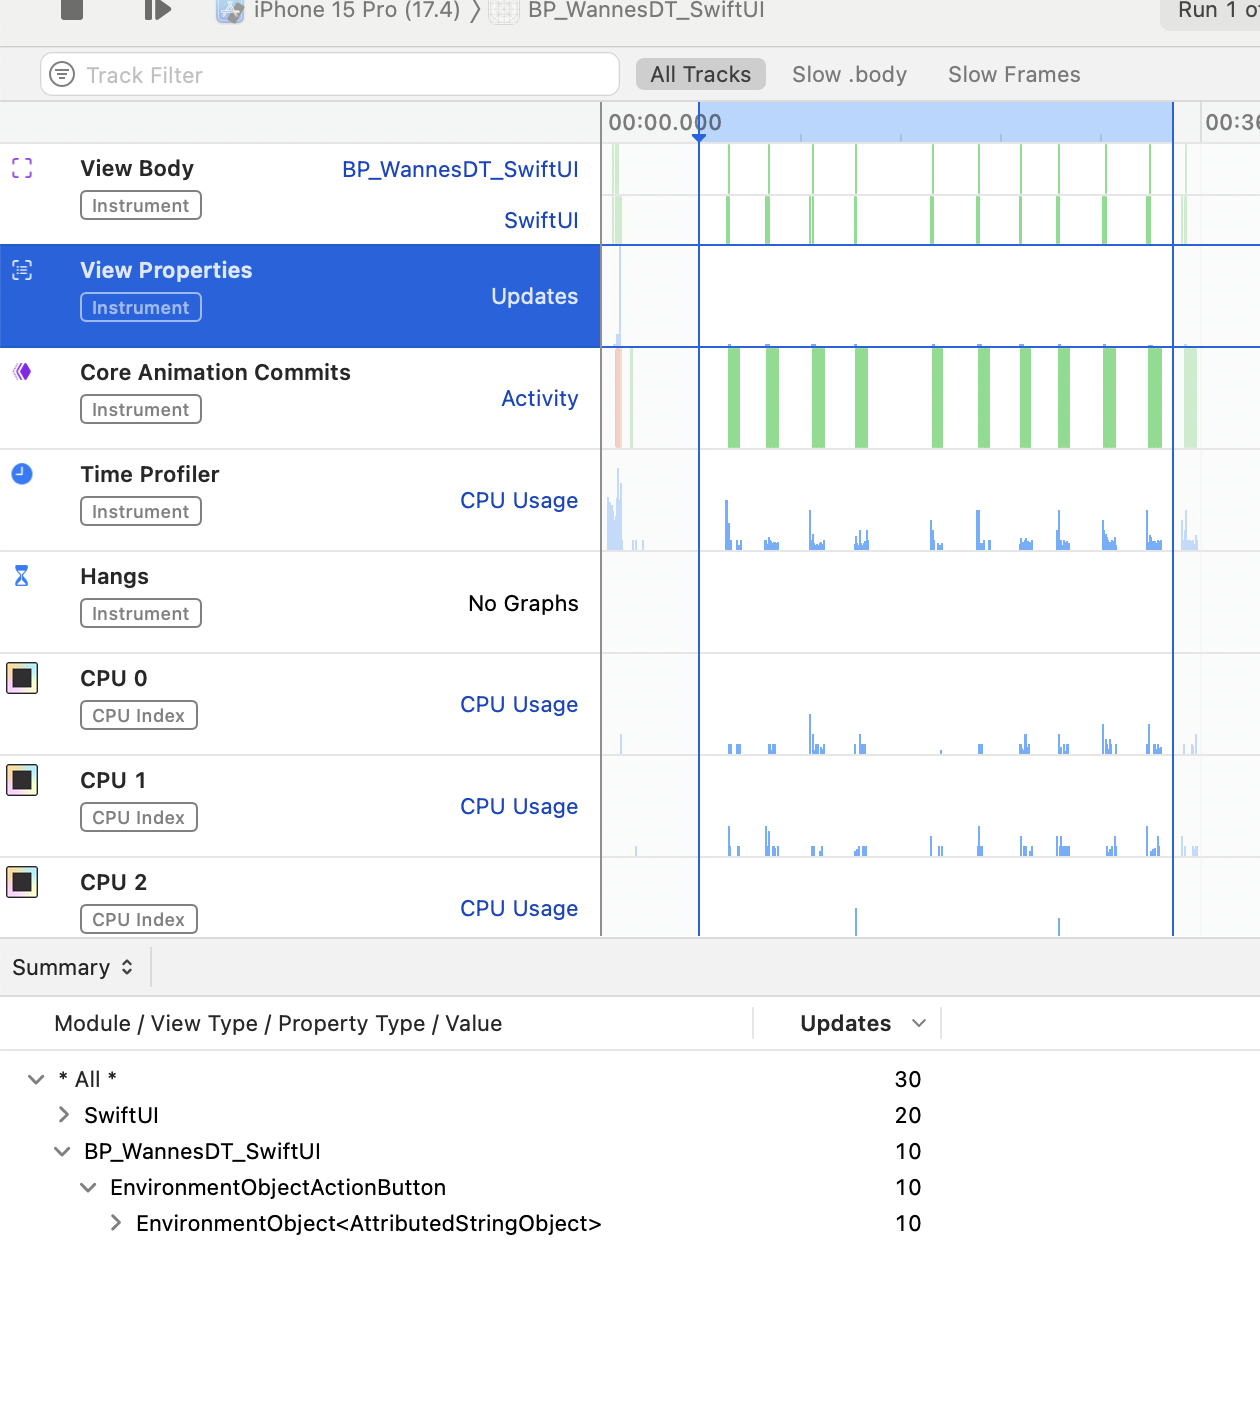
\includegraphics[width=0.7\textwidth]{bptest1_insubview/EnvironnmentObjectButtonPressViewPropertyUpdates} 
    \caption{test2: Aantal keren dat de property's updaten bij het meervoudig toewijzigen van een EnvironmentObject}
    \label{fig:propertyUpdatesEnvironmentObject1}
\end{figure}
\paragraph{Totale tijd gebruikt van de CPU}
\begin{figure}[H]
    \centering
    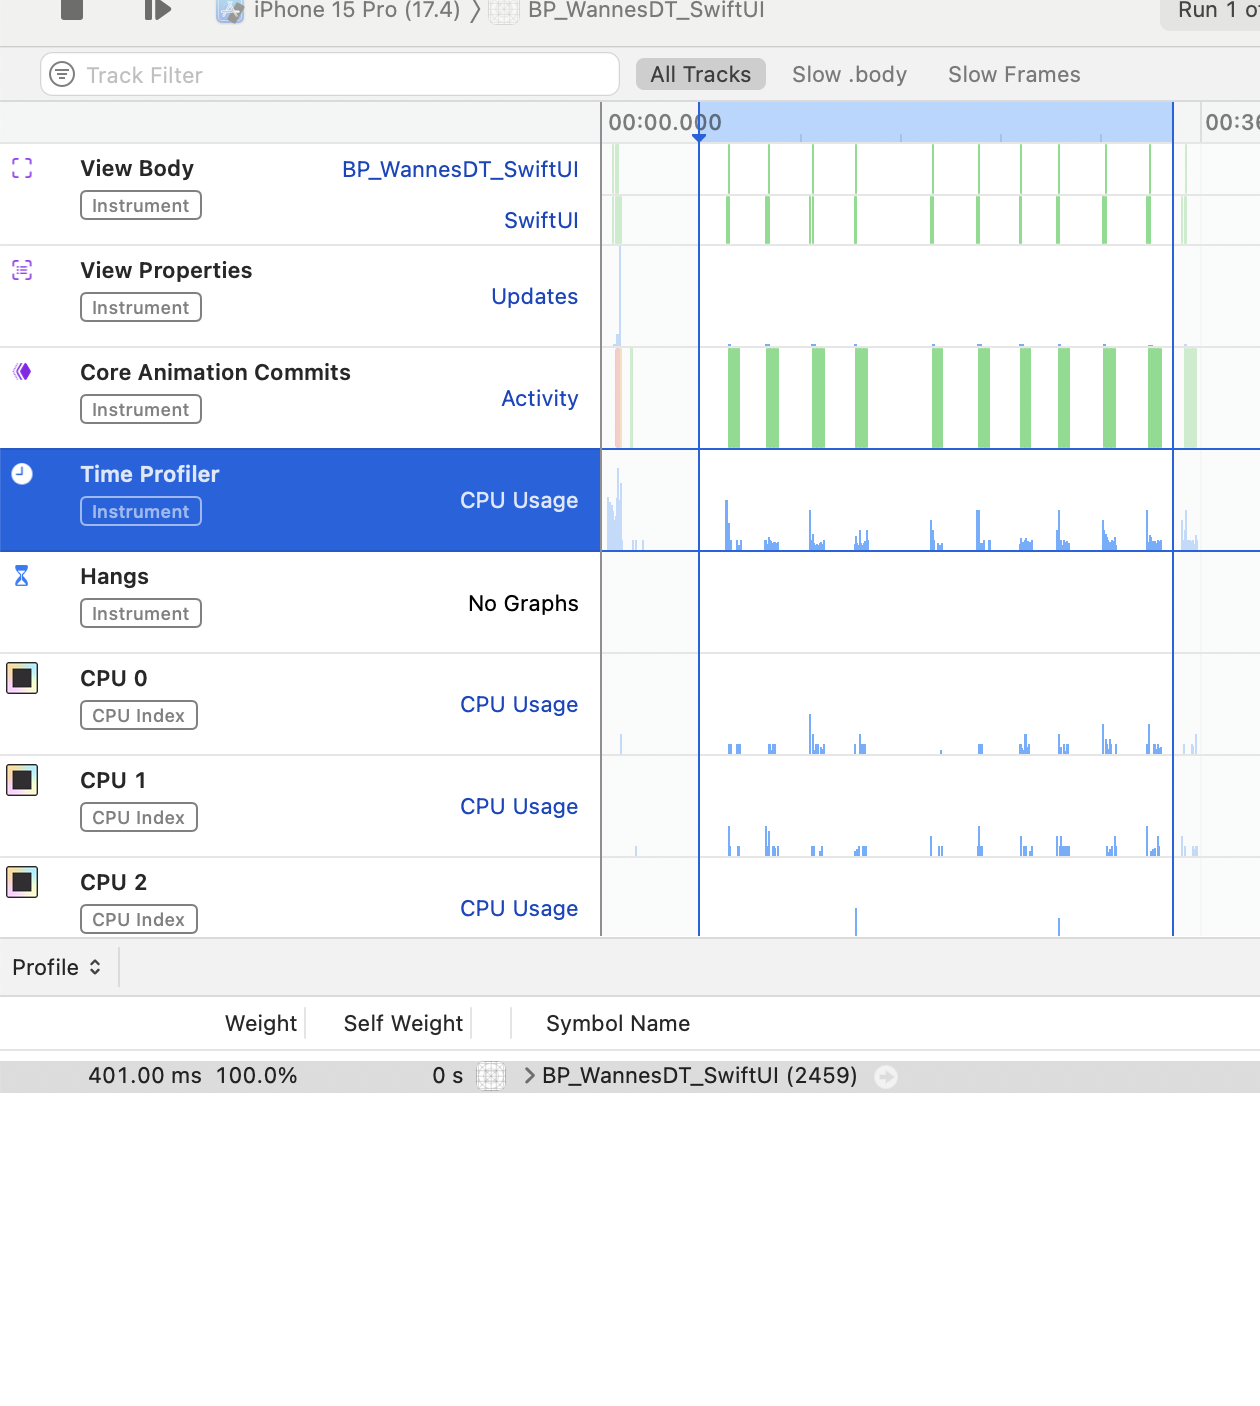
\includegraphics[width=0.7\textwidth]{bptest1_insubview/EnvironmentObjectButtonPressTotalCpuTime} 
    \caption{test2: De totale duratie die gebruikt is van de CPU bij het gebruik van EnvironmentObject}
    \label{fig:cpuUsageTimeEnvironmentObject1}
\end{figure}
\paragraph{Last op de CPU}
\begin{figure}[H]
    \centering
    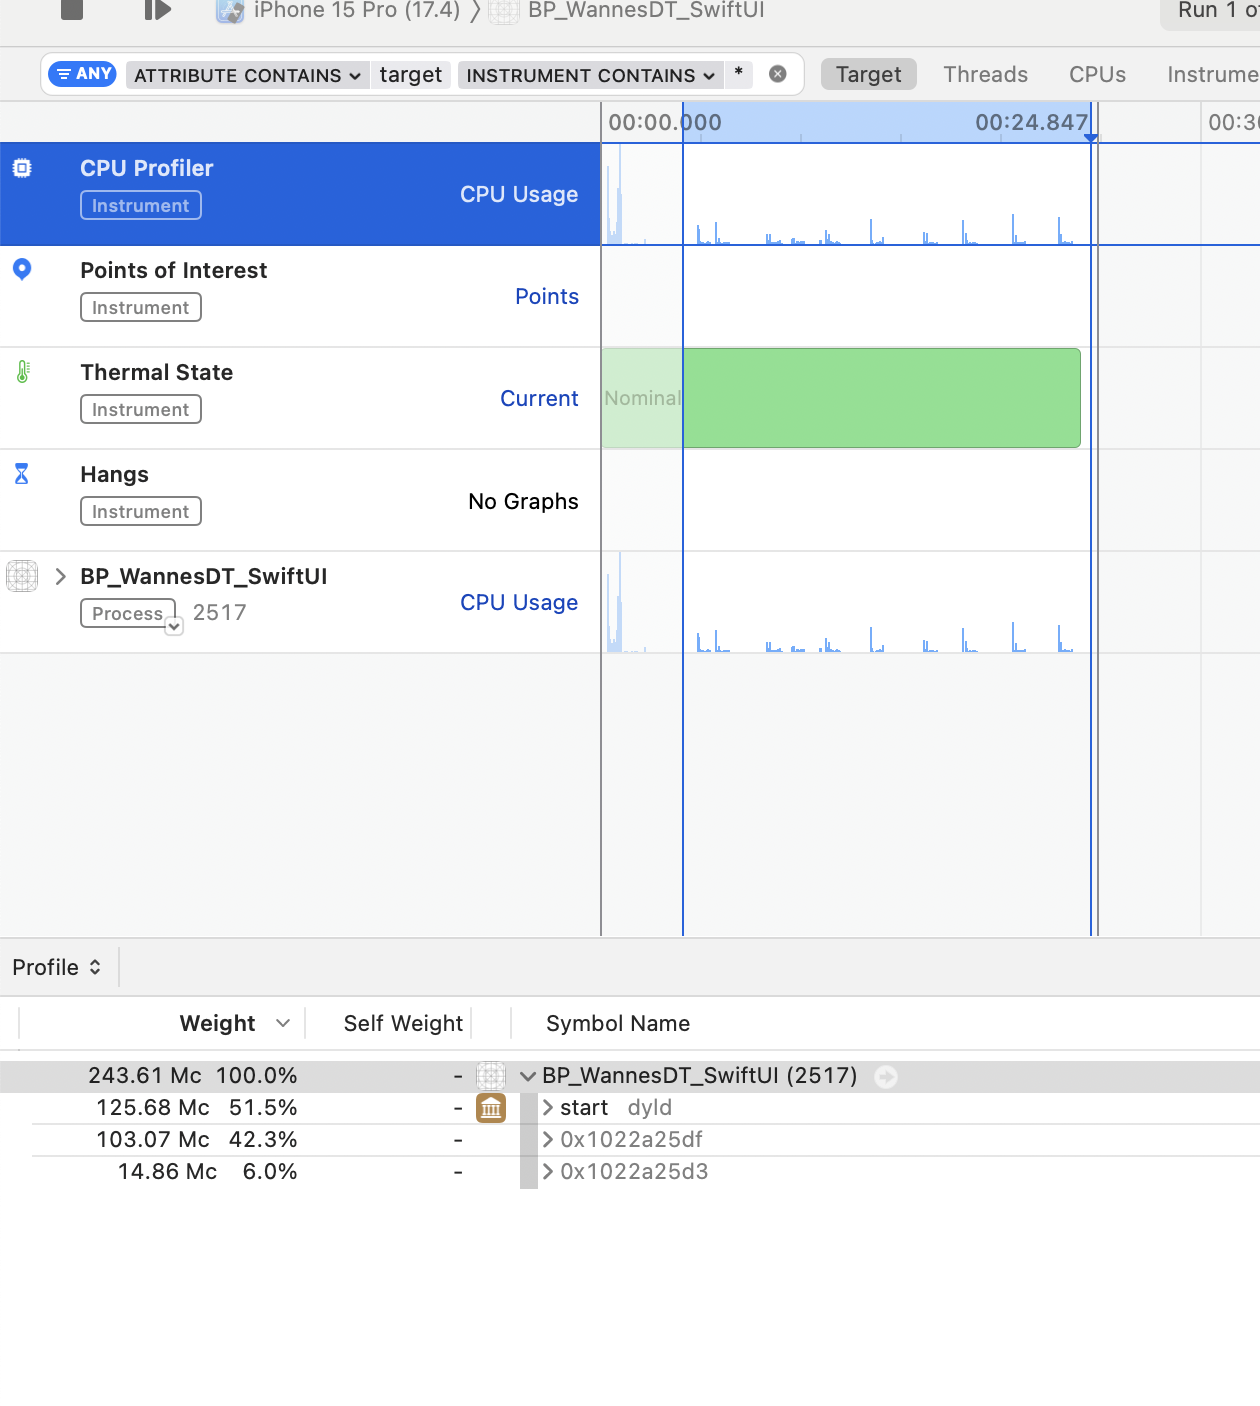
\includegraphics[width=0.7\textwidth]{bptest1_insubview/EnvironmentObjectButtonPressCpuUsage} 
    \caption{test2: De totale last van het opnieuw toewijzen van property's op de cpu bij het gebruik van EnvironmentObject}
    \label{fig:cpuWeightEnvironmentObject1}
\end{figure}

\section{Test3: Dataoverdracht naar meerdere subview's met lazyLists}
% Binding test 2
In dit hoofdstuk word de applicatie in de afbeelding hieronder gebruikt om de testen uit te voeren. Opgebouwd uit 1 LazyVStack's die 10 LazyHStack's bevat per HStack worden er 10 Tegels weergegeven. Elke tegel is zeer CPU heavy opgebouwd zodat de resultaten meer zichtbaar worden in de testen. Elke tile bevat ook een knop die een aanpassing van de testbare data gaat triggeren. In volgende afbeelding word de hierarchy afgebeeld. Voor elk type van dataoverdracht is er 10 keer op de button gedrukt voor het wijzigen van de view. Zo zijn de metingen tot stand gekomen. Alle ruwe resultaten die waargenomen zijn per datatype kan u terugvinden in onderstaande sectie's en afbeeldingen.
\begin{figure}[htbp]
    \centering
    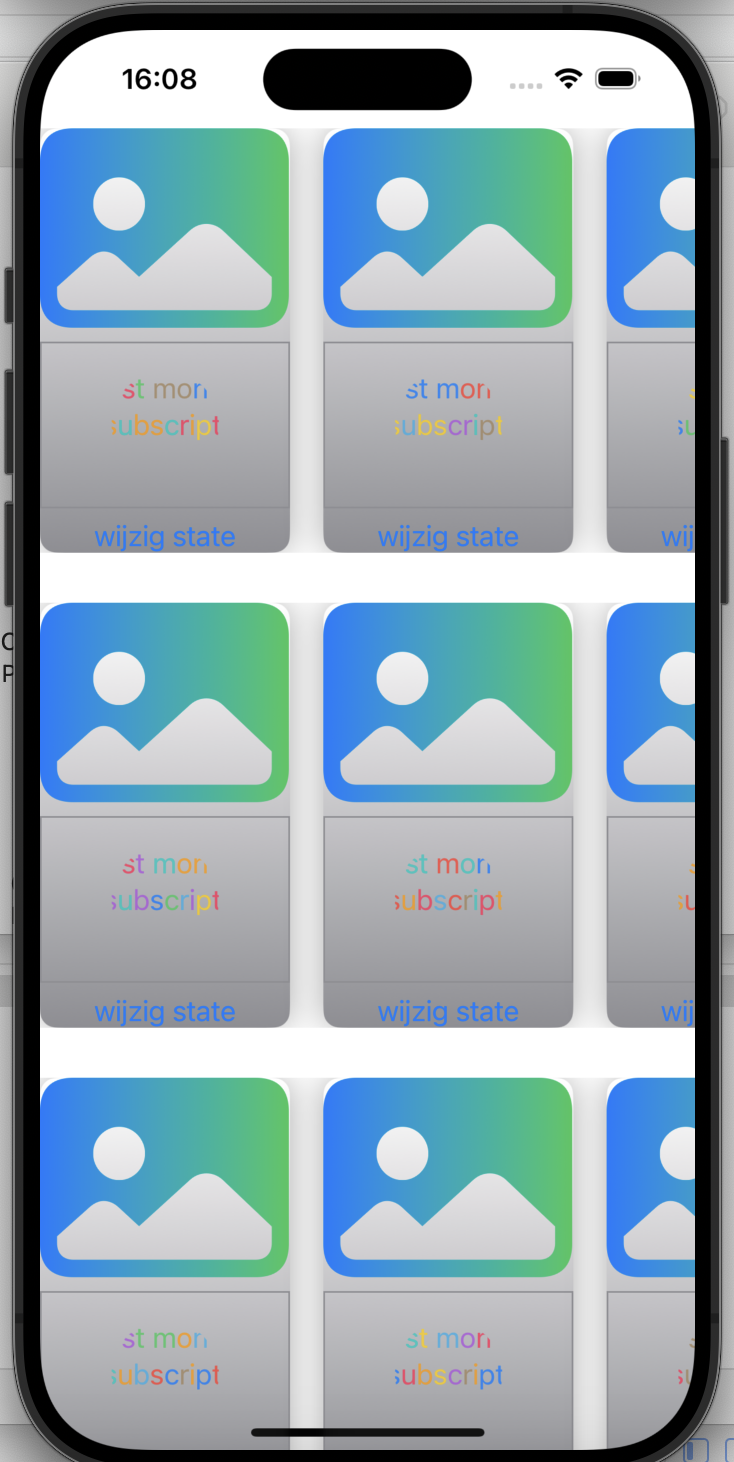
\includegraphics[width=0.4\textwidth]{testapplication} 
    \caption{testapplicatie}
    \label{fig:testapplication2}
\end{figure}
\begin{figure}[htbp]
    \centering
    \includegraphics[width=0.4\textwidth]{bptest2_lazy/dataHierarchy} 
    \caption{testapplicatie data hierarchy}
    \label{fig:testapplicationHierarchy2}
\end{figure}
\subsection{Binding}
\paragraph{View ververs aantal en ververs tijd}
\begin{figure}[H]
    \centering
    \includegraphics[width=0.7\textwidth]{BPtest2_lazy/BindingViewRefreshes} 
    \caption{test3: Aantal keren dat de view refreshed en gemiddelde duratie bij het meervoudig toewijzigen van een binding}
    \label{fig:viewRefreshesBinding2}
\end{figure}
\paragraph{Aantal updates van property's}
\begin{figure}[H]
    \centering
    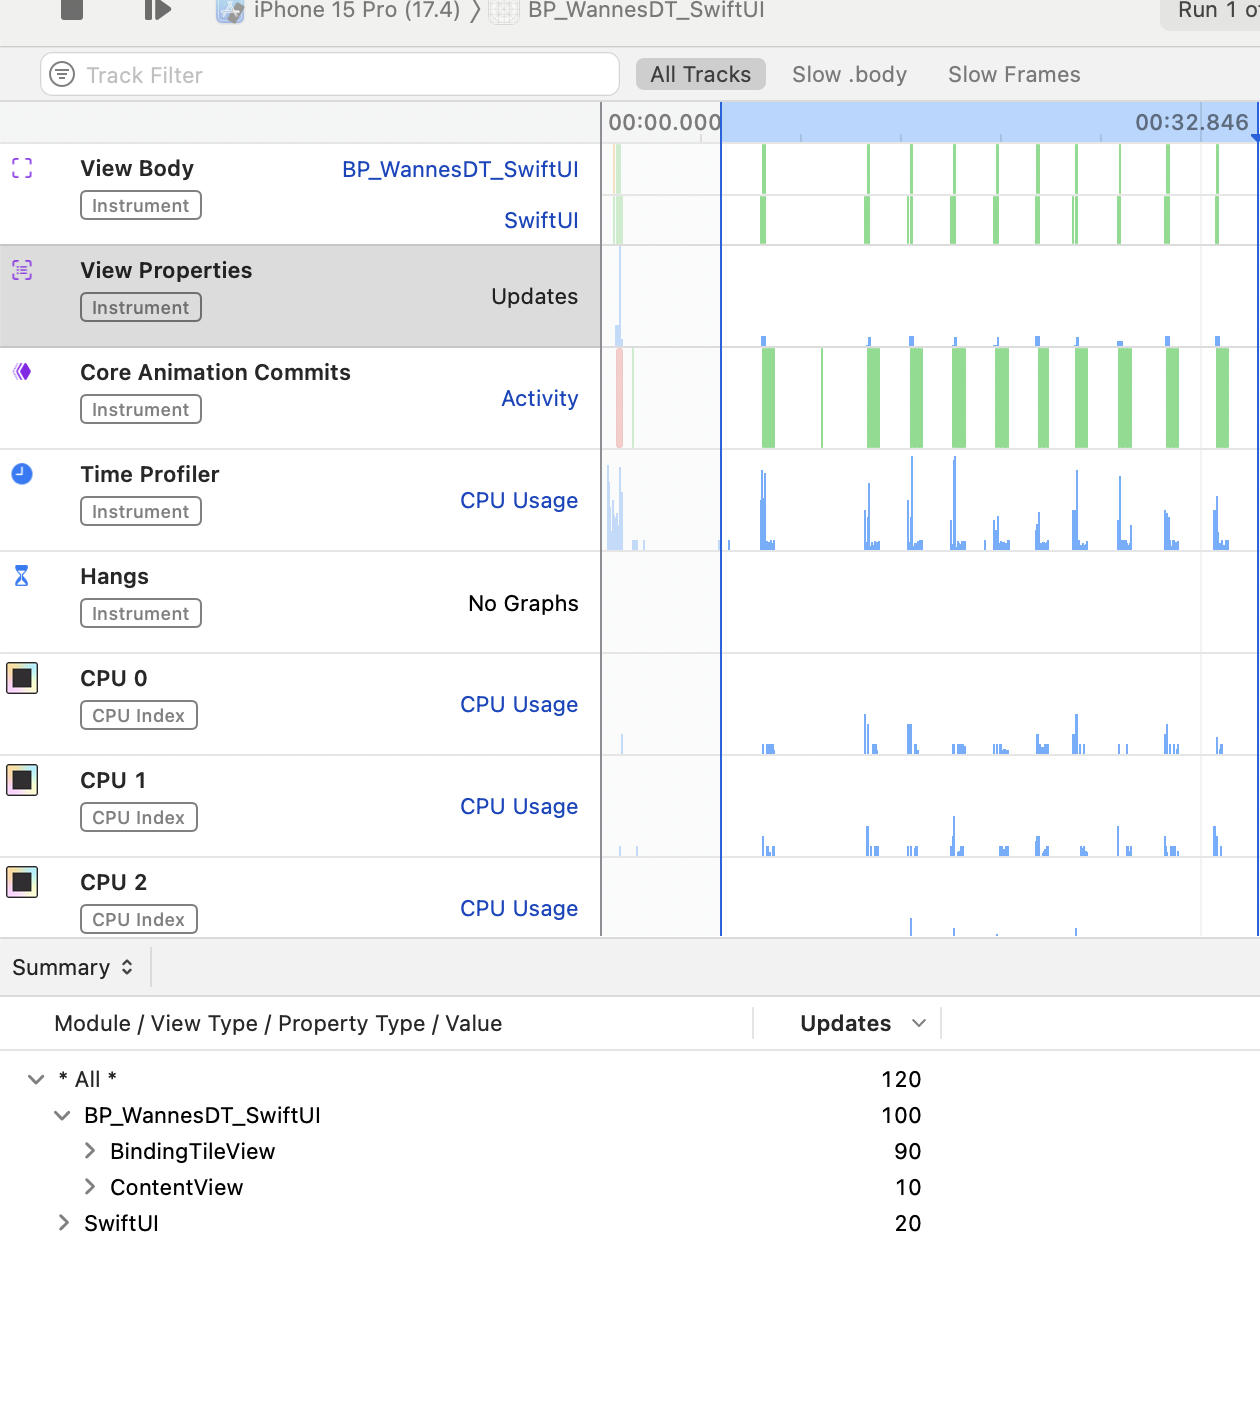
\includegraphics[width=0.7\textwidth]{BPtest2_lazy/BindingPropertyUpdates} 
    \caption{test3: Aantal keren dat de property's updaten bij het meervoudig toewijzigen van een binding}
    \label{fig:propertyUpdatesBinding2}
\end{figure}
\paragraph{Totale tijd gebruikt van de CPU}
\begin{figure}[H]
    \centering
    \includegraphics[width=0.7\textwidth]{BPtest2_lazy/BindingTotalCpuTime} 
    \caption{test3: De totale duratie die gebruikt is van de CPU bij het gebruik van bindings}
    \label{fig:cpuUsageTimeBinding2}
\end{figure}
\paragraph{Last op de CPU}
\begin{figure}[H]
    \centering
    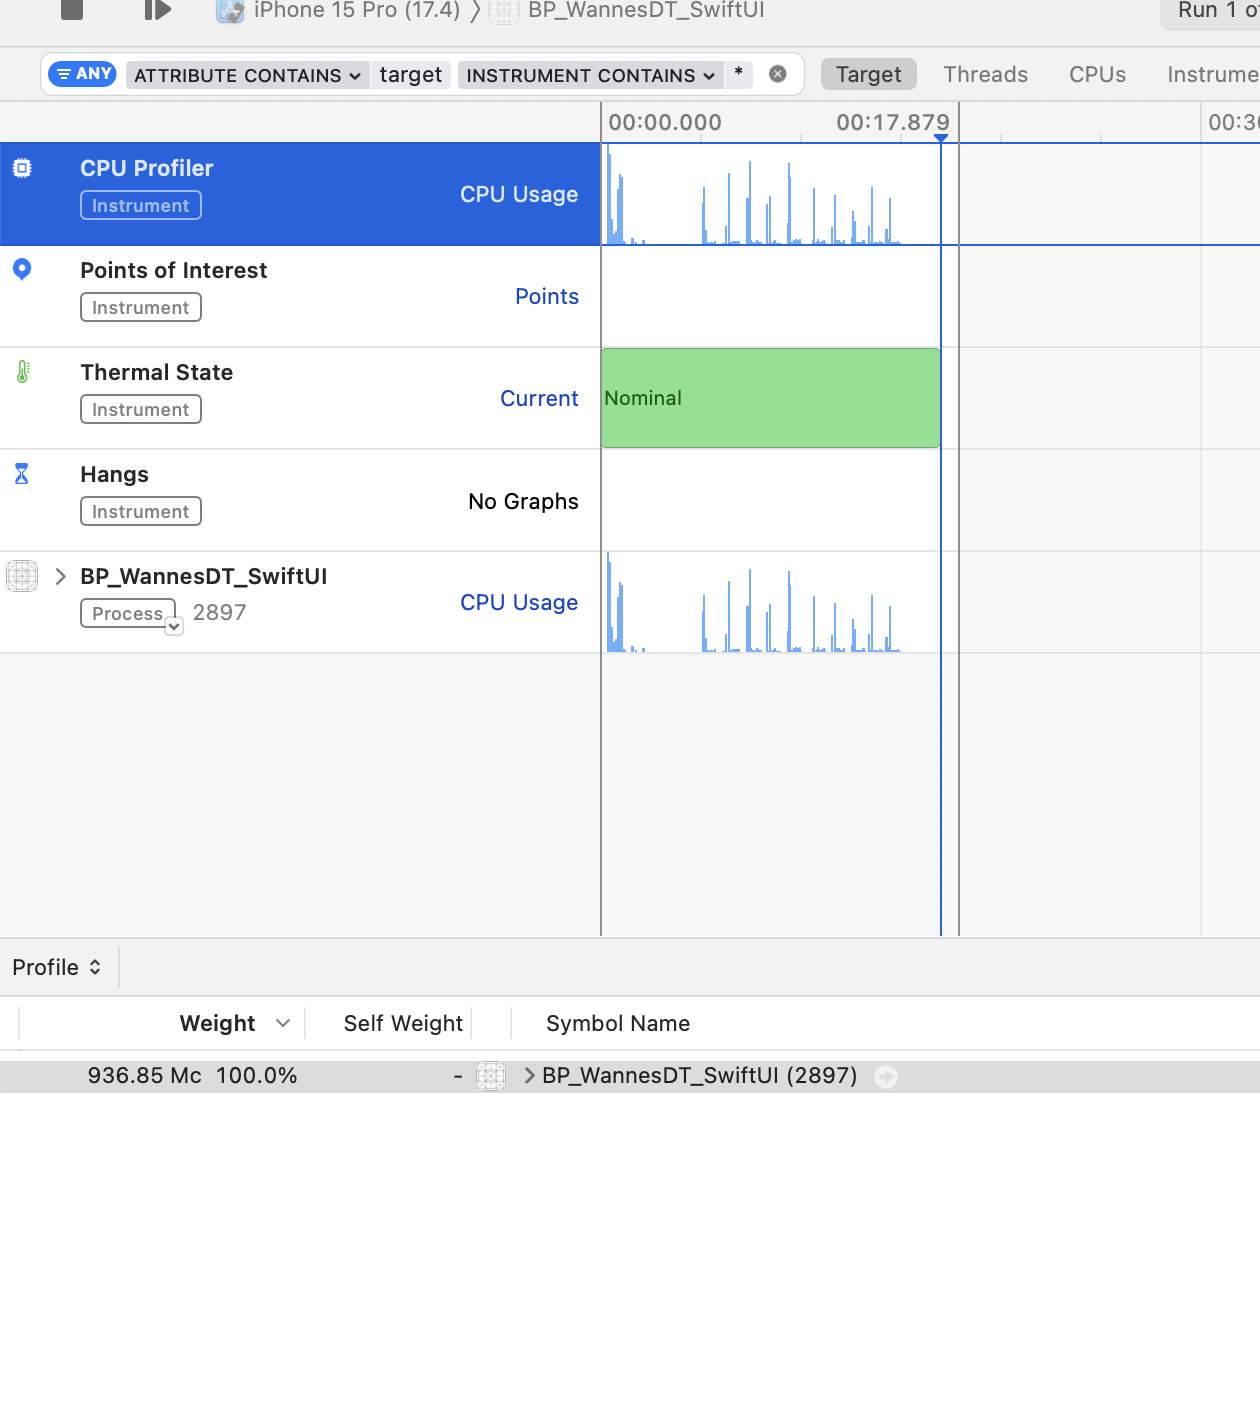
\includegraphics[width=0.7\textwidth]{BPtest2_lazy/BindingCpuWeight} 
    \caption{test3: De totale last van het opnieuw toewijzen van property's op de cpu bij het gebruik van bindings}
    \label{fig:cpuWeightBinding2}
\end{figure}

% Observable test 2
\subsection{Observable}
\paragraph{View ververs aantal en ververs tijd}
\begin{figure}[H]
    \centering
    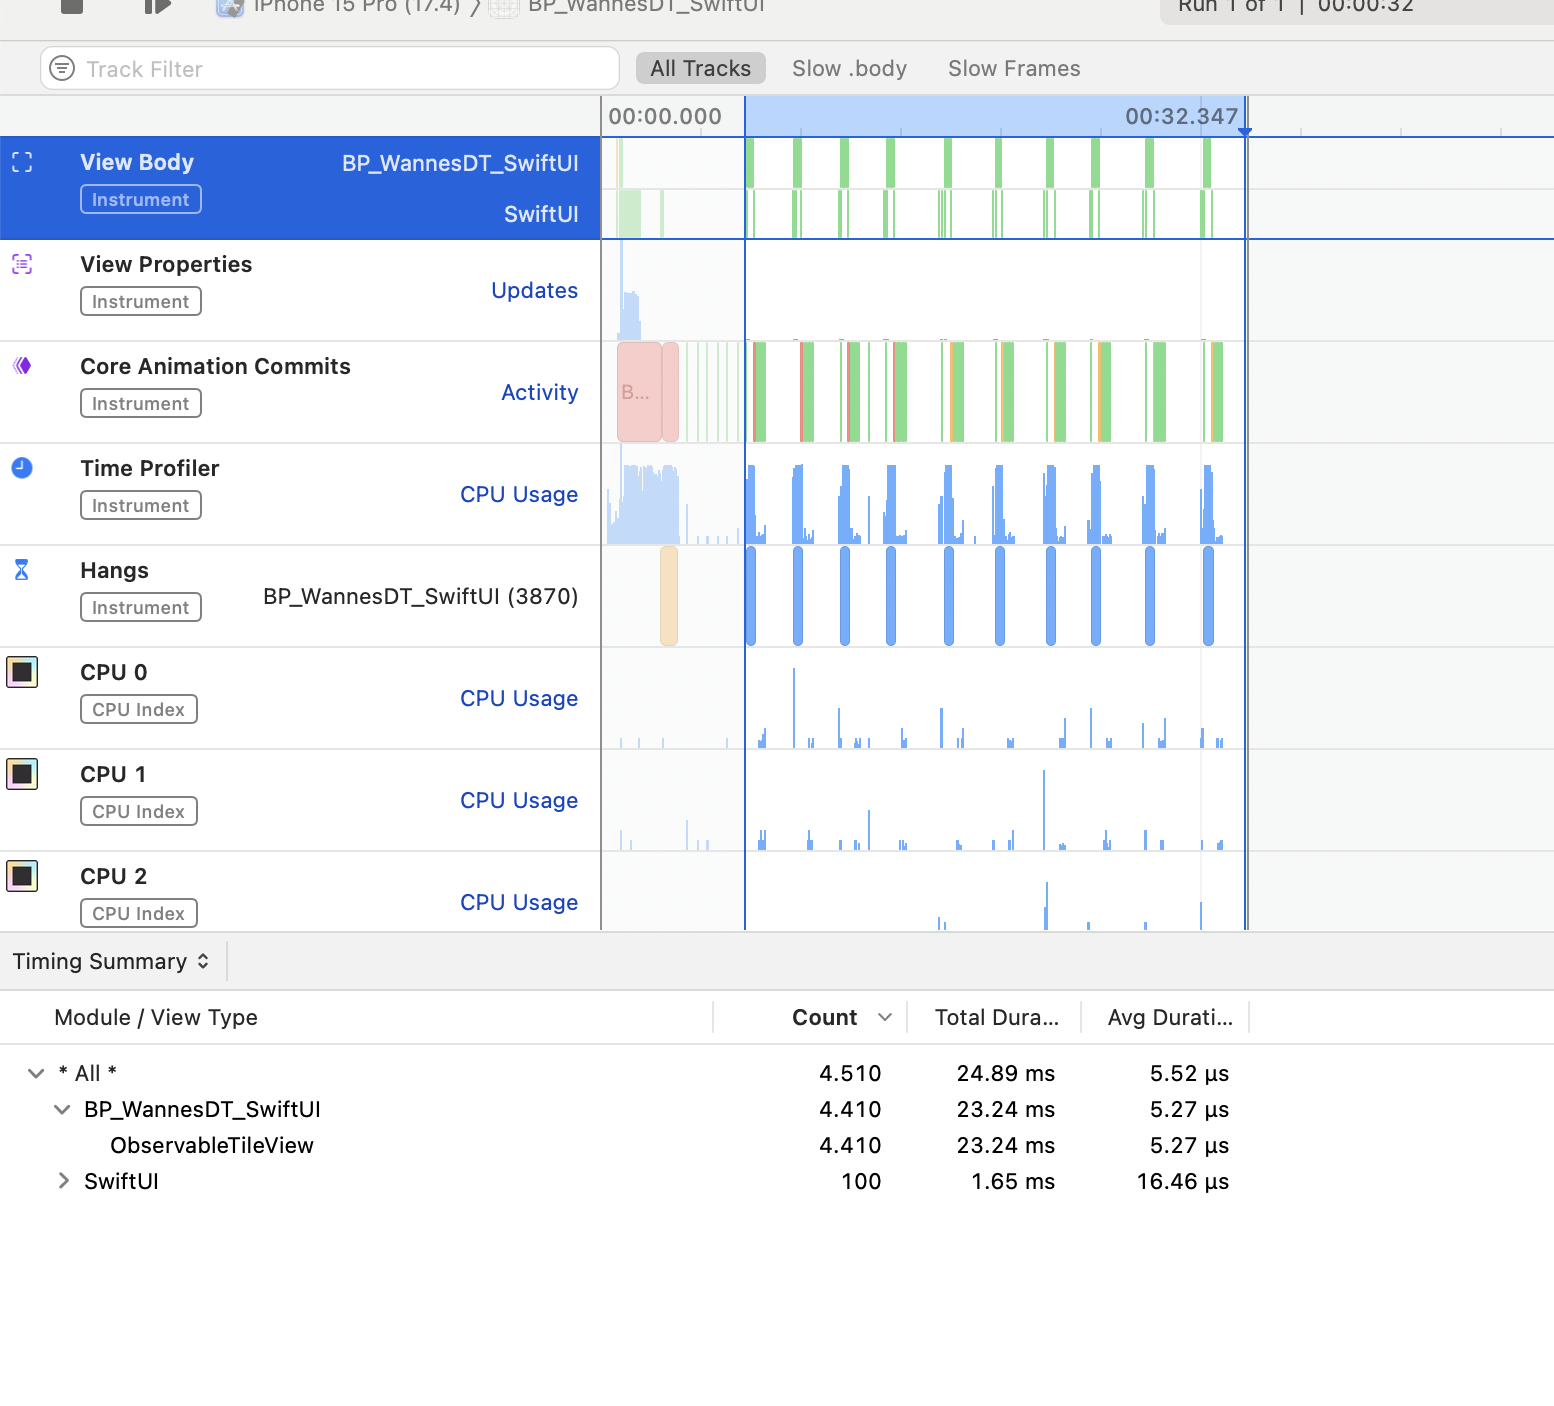
\includegraphics[width=0.7\textwidth]{BPtest2_lazy/ObservableViewRefreshes} 
    \caption{test3: Aantal keren dat de view refreshed en gemiddelde duratie bij het meervoudig toewijzigen van een Observable}
    \label{fig:viewRefreshesObservable2}
\end{figure}
\paragraph{Aantal updates van property's}
\begin{figure}[H]
    \centering
    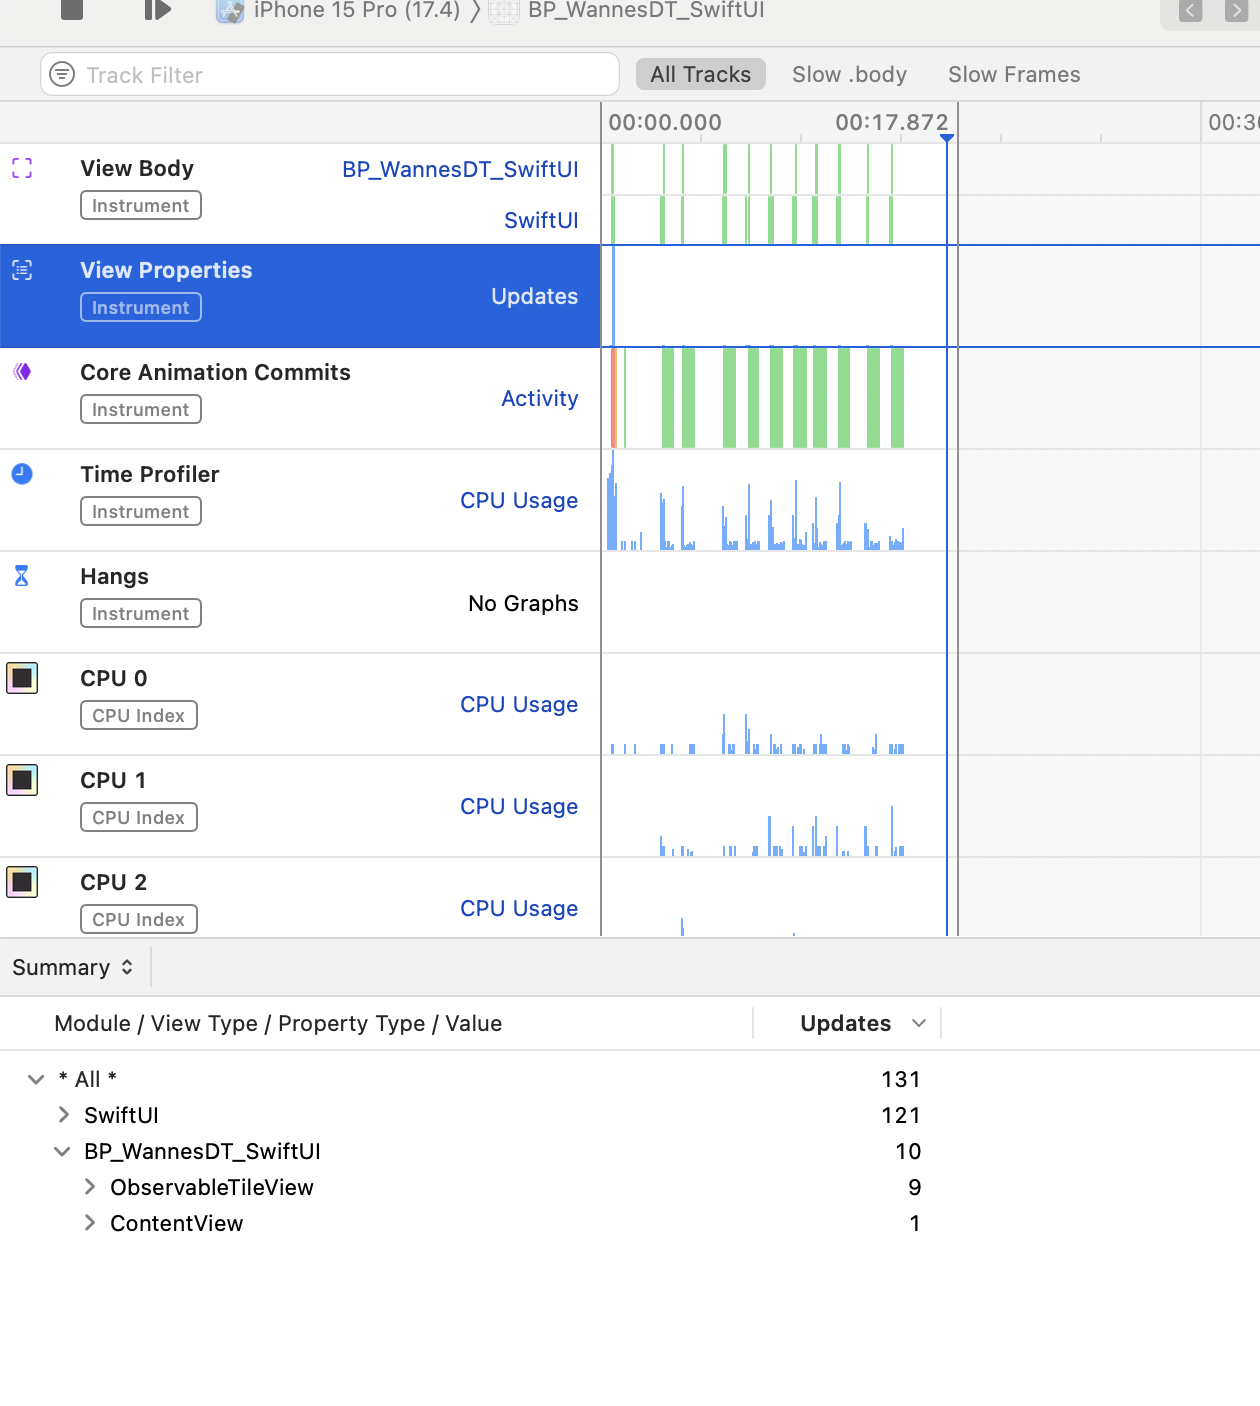
\includegraphics[width=0.7\textwidth]{BPtest2_lazy/ObservablePropertyUpdates} 
    \caption{test3: Aantal keren dat de property's updaten bij het meervoudig toewijzigen van een Observable}
    \label{fig:propertyUpdatesObservable2}
\end{figure}
\paragraph{Totale tijd gebruikt van de CPU}
\begin{figure}[H]
    \centering
    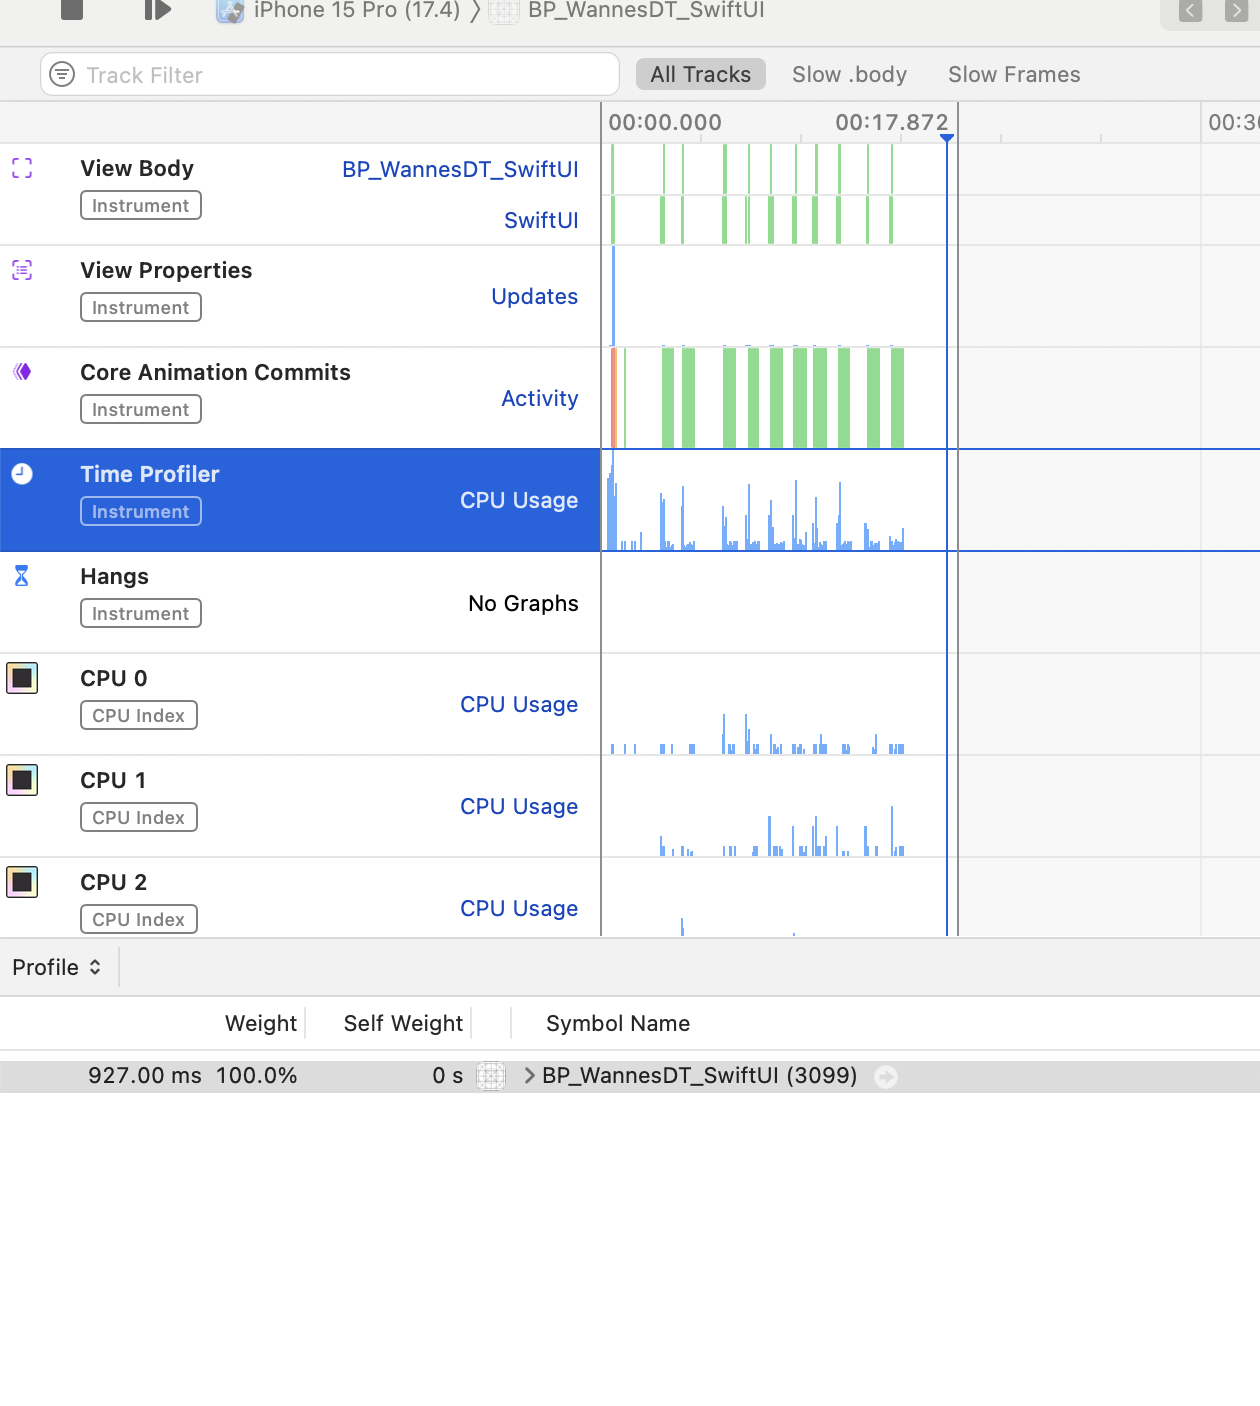
\includegraphics[width=0.7\textwidth]{BPtest2_lazy/ObservableTotalCpuTime} 
    \caption{test3: De totale duratie die gebruikt is van de CPU bij het gebruik van Observable's}
    \label{fig:cpuUsageTimeObservable2}
\end{figure}
\paragraph{Last op de CPU}
\begin{figure}[H]
    \centering
    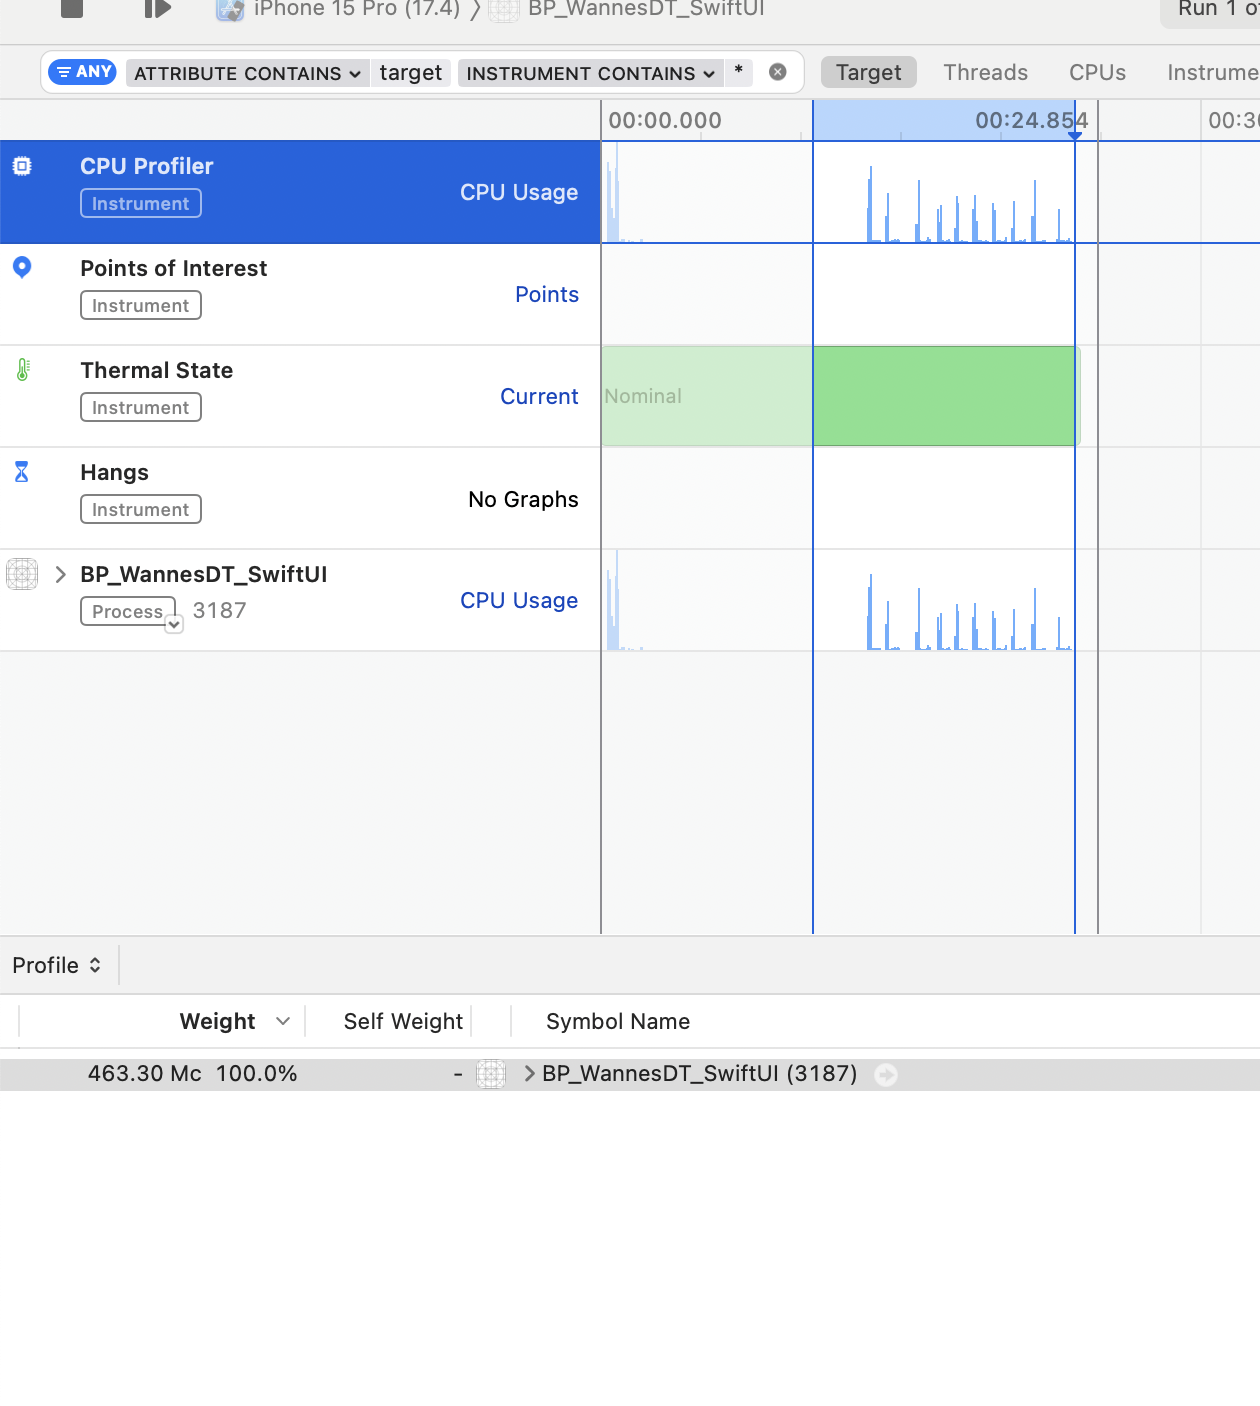
\includegraphics[width=0.7\textwidth]{BPtest2_lazy/ObservableCpuWieght} 
    \caption{test3: De totale last van het opnieuw toewijzen van property's op de cpu bij het gebruik van Observable's}
    \label{fig:cpuWeightObservable2}
\end{figure}

% ObservedObject test 2
\subsection{ObservedObject}
\paragraph{View ververs aantal en ververs tijd}
\begin{figure}[H]
    \centering
    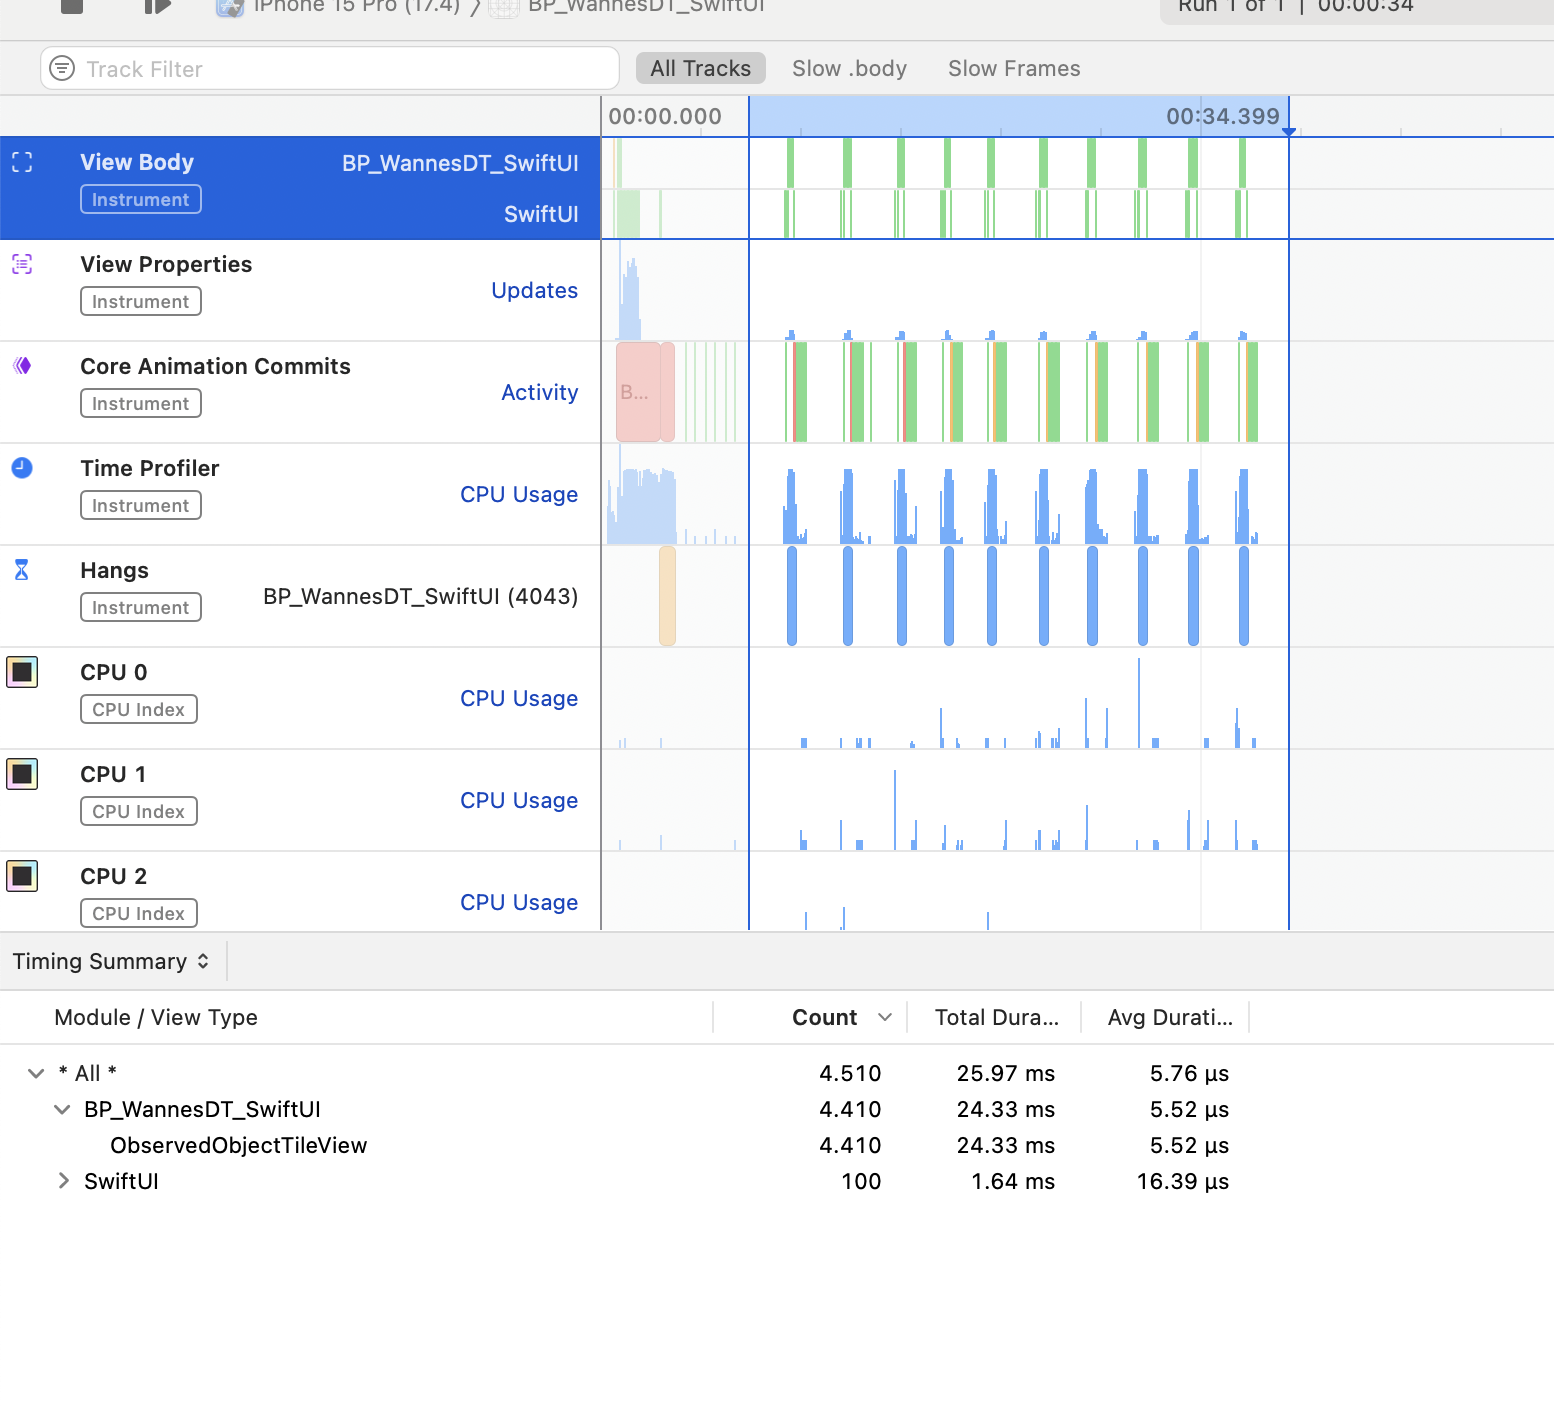
\includegraphics[width=0.7\textwidth]{BPtest2_lazy/ObservedObjectViewRefreshes} 
    \caption{test3: Aantal keren dat de view refreshed en gemiddelde duratie bij het meervoudig toewijzigen van een ObservedObject}
    \label{fig:viewRefreshesObservedObject2}
\end{figure}
\paragraph{Aantal updates van property's}
\begin{figure}[H]
    \centering
    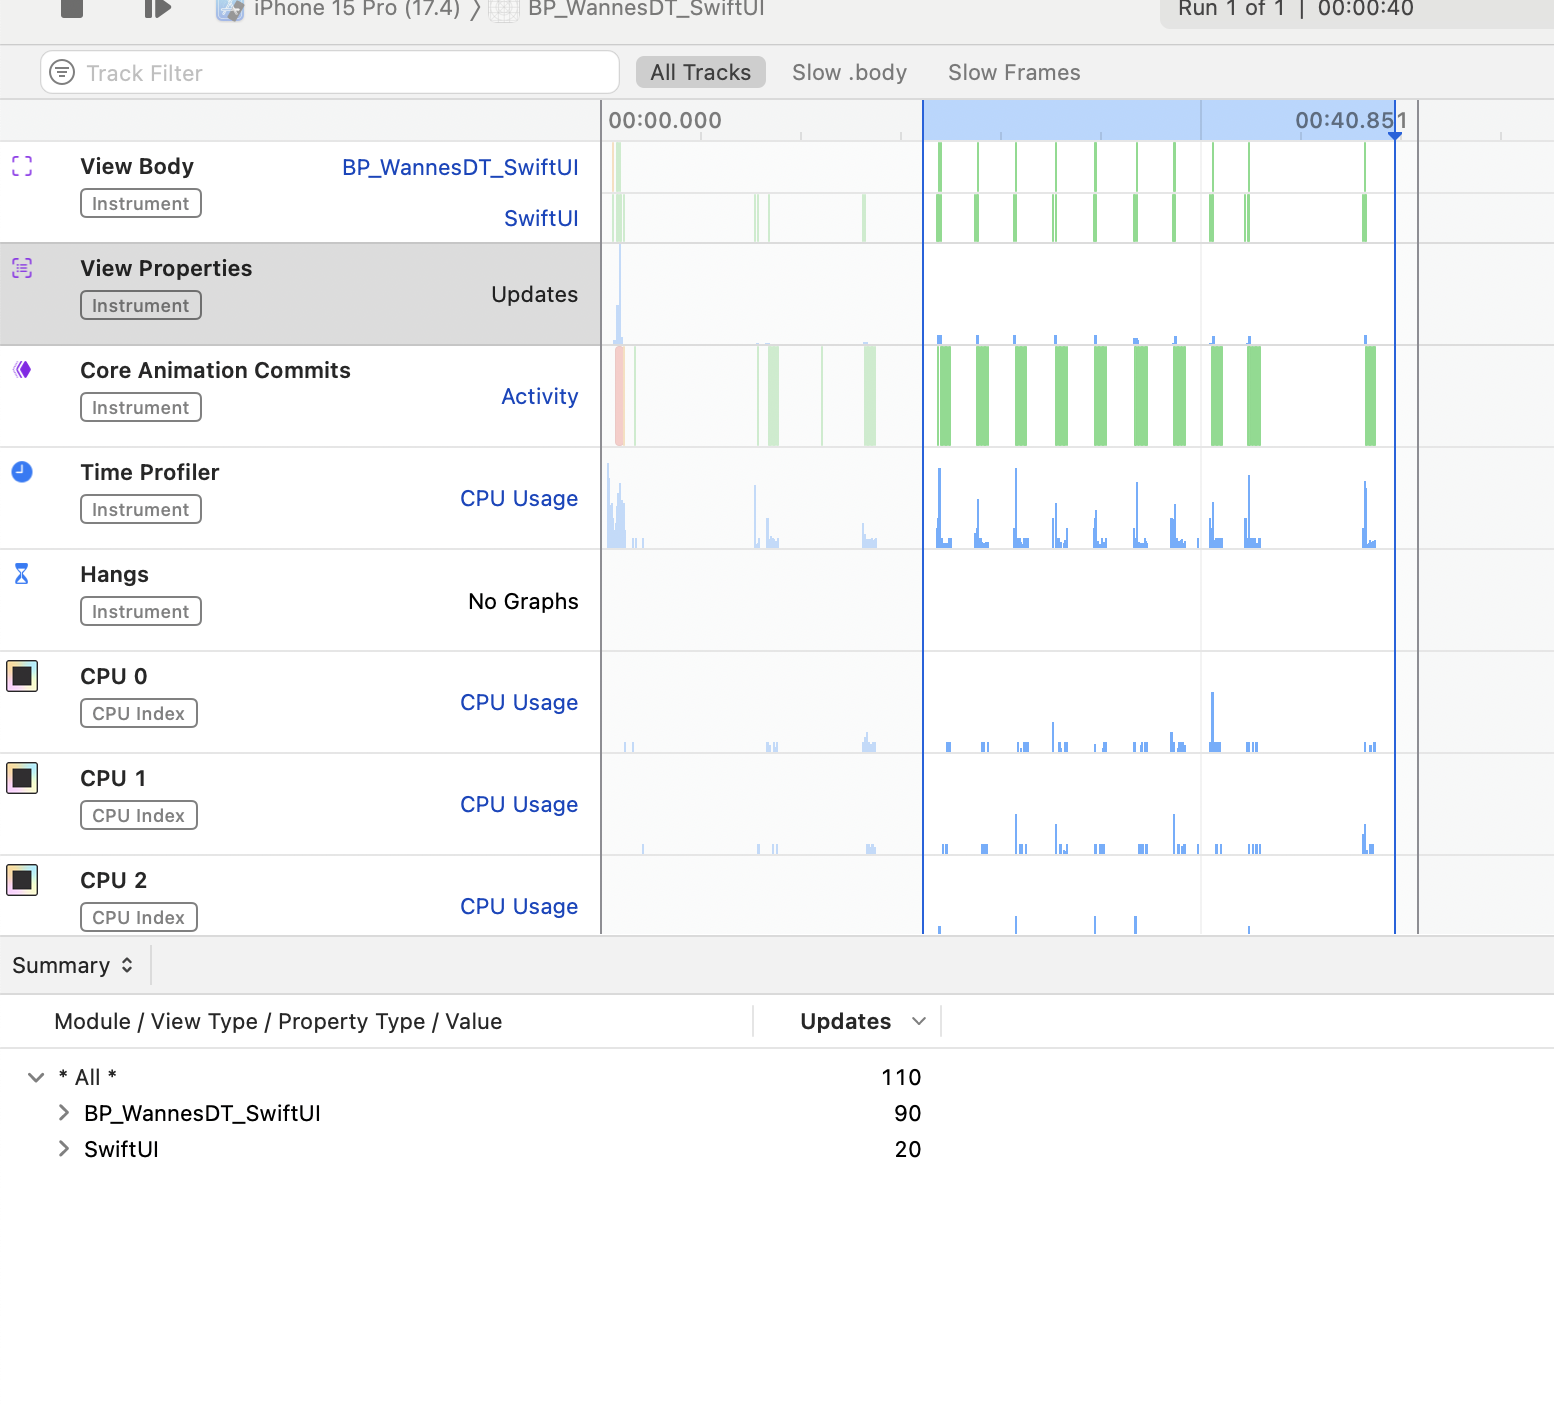
\includegraphics[width=0.7\textwidth]{BPtest2_lazy/ObservedObjectPropertyUpdates} 
    \caption{test3: Aantal keren dat de property's updaten bij het meervoudig toewijzigen van een ObservedObject}
    \label{fig:propertyUpdatesObservedObject2}
\end{figure}
\paragraph{Totale tijd gebruikt van de CPU}
\begin{figure}[H]
    \centering
    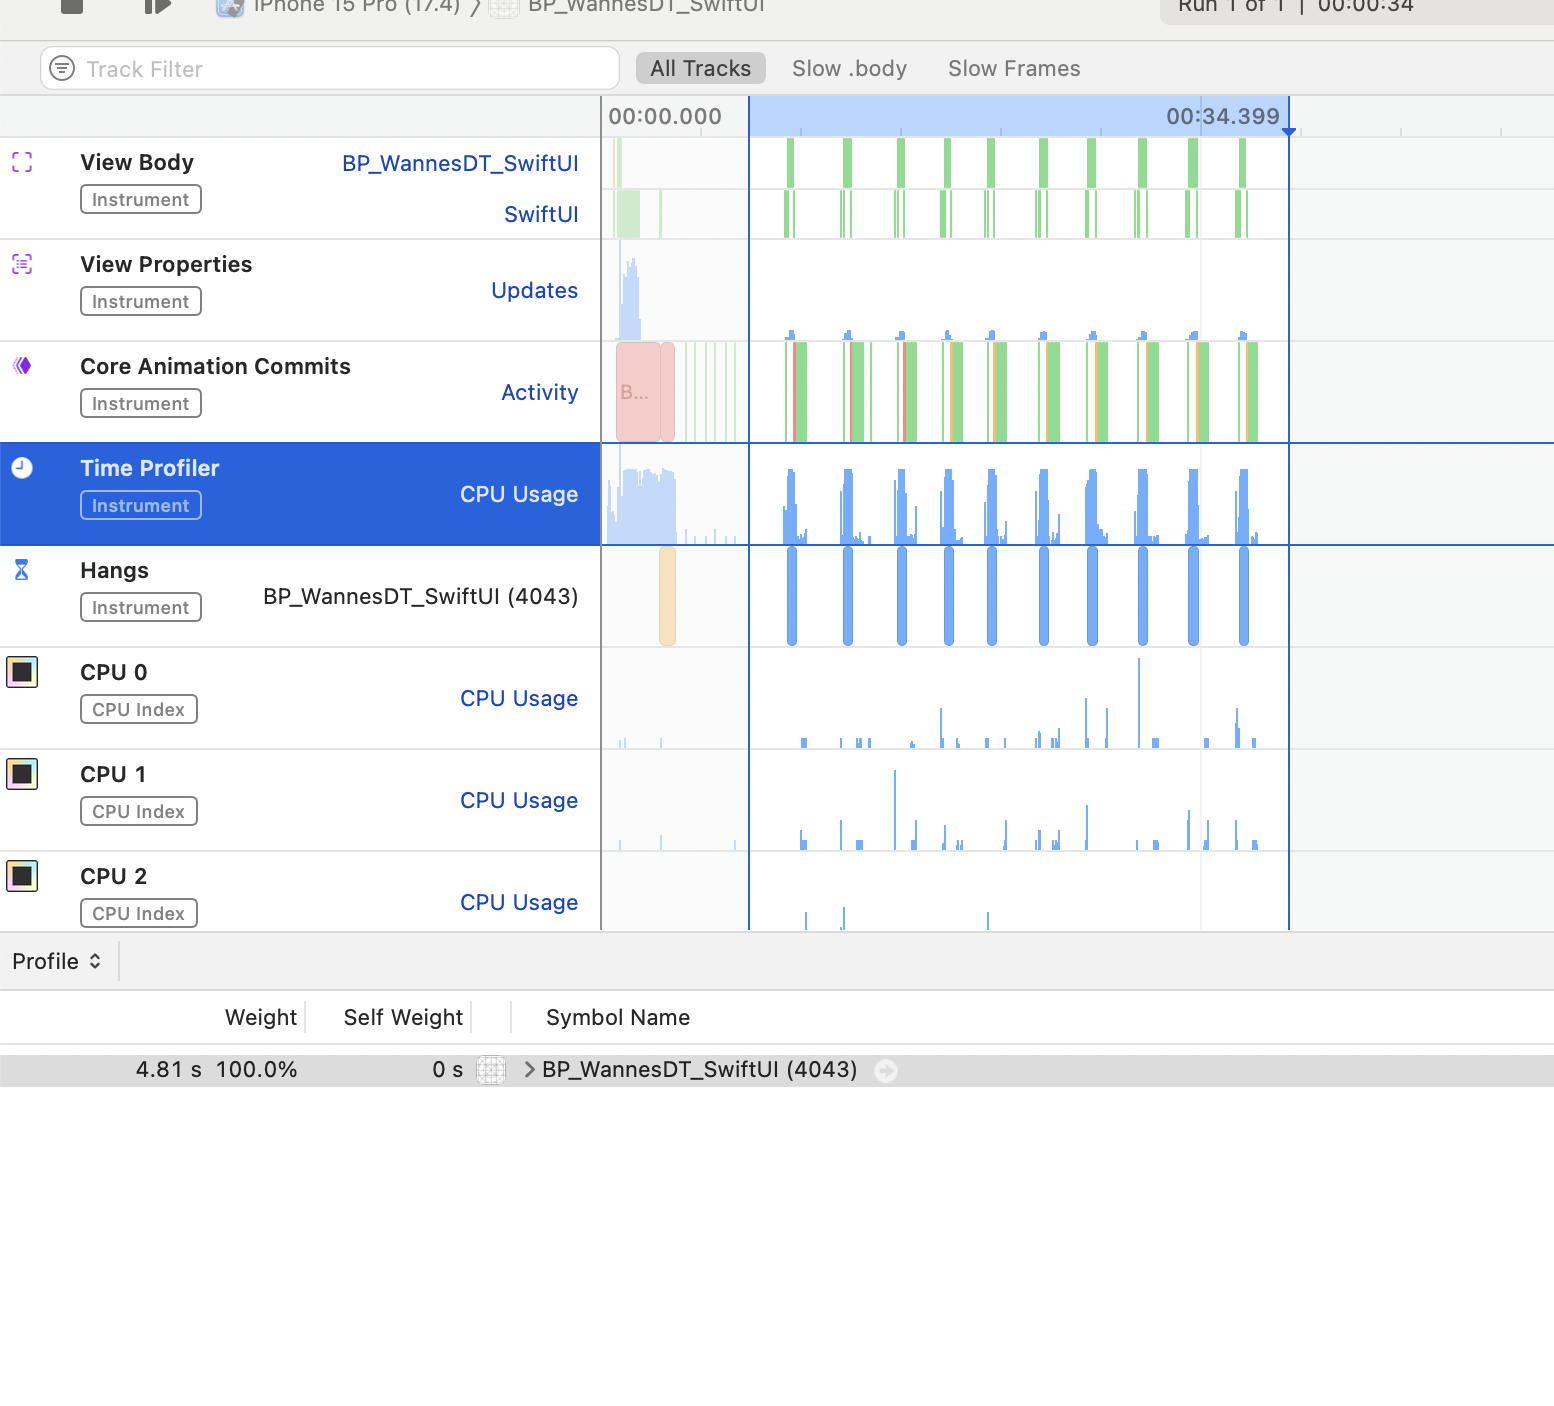
\includegraphics[width=0.7\textwidth]{BPtest2_lazy/ObservedObjectTotalCpuTime} 
    \caption{test3: De totale duratie die gebruikt is van de CPU bij het gebruik van ObservedObject's}
    \label{fig:cpuUsageTimeObservedObject2}
\end{figure}
\paragraph{Last op de CPU}
\begin{figure}[H]
    \centering
    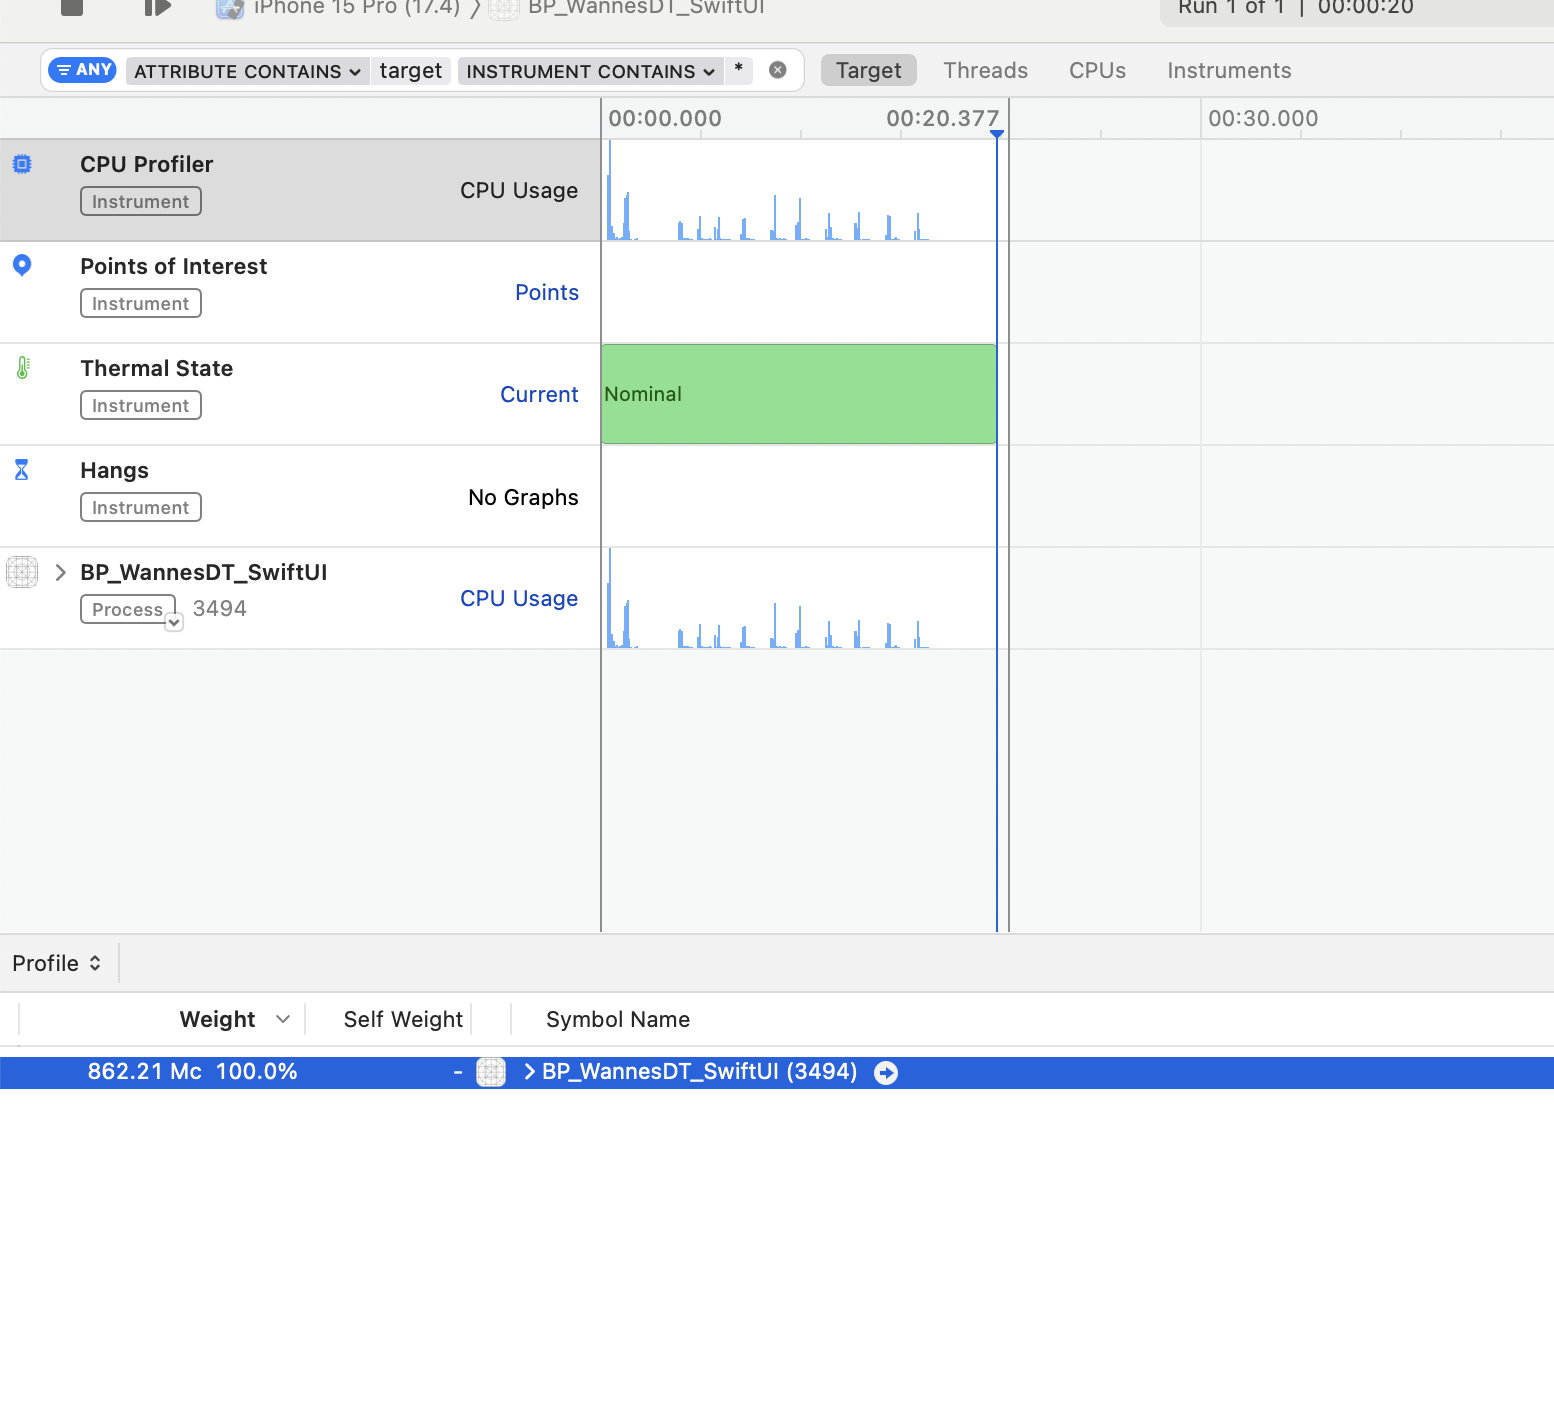
\includegraphics[width=0.7\textwidth]{BPtest2_lazy/ObservedObjectCpuWieght} 
    \caption{test3: De totale last van het opnieuw toewijzen van property's op de cpu bij het gebruik van ObservedObject's}
    \label{fig:cpuWeightObservedObject2}
\end{figure}

% EnvironmentObject test 2
\subsection{EnvironmentObject}
\paragraph{View ververs aantal en ververs tijd}
\begin{figure}[H]
    \centering
    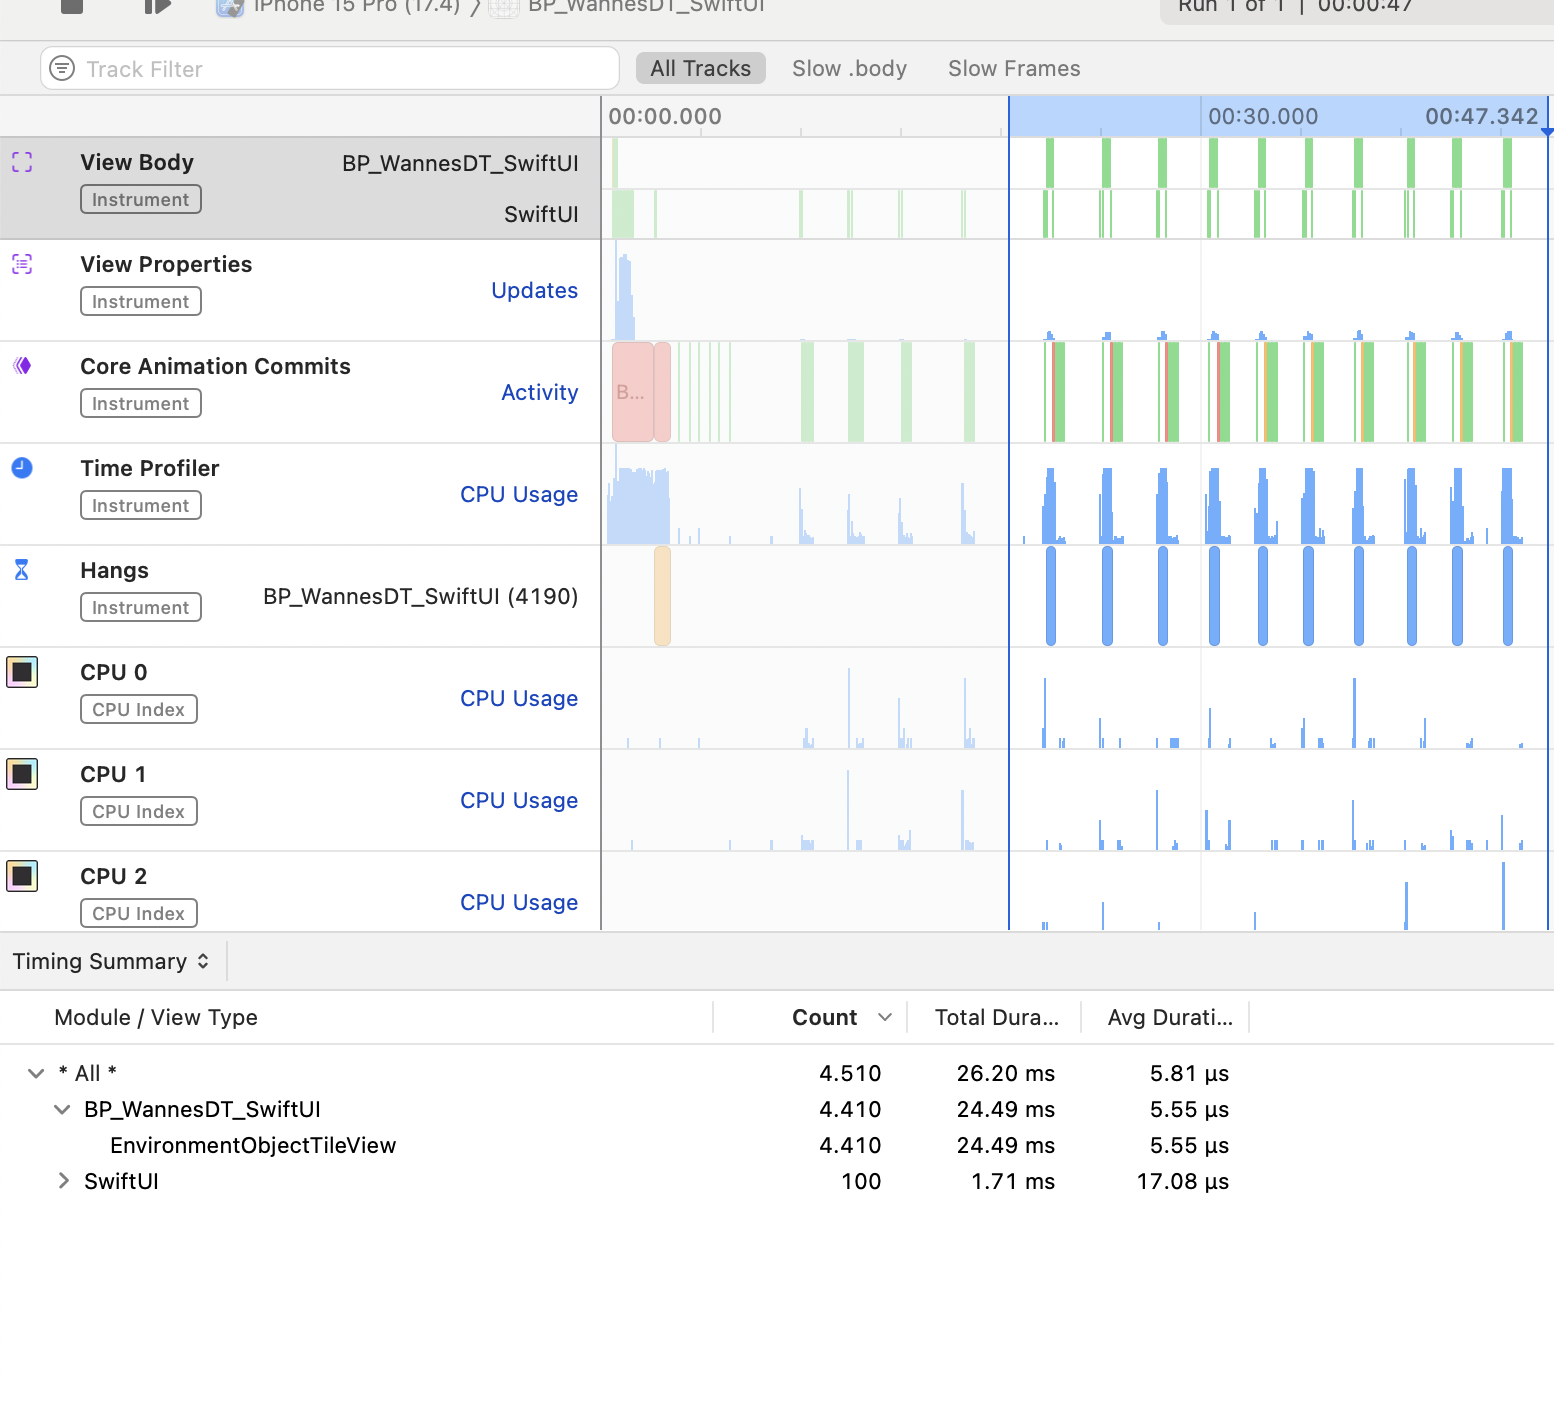
\includegraphics[width=0.7\textwidth]{BPtest2_lazy/EnvironmentObjectViewRefreshes} 
    \caption{test3: Aantal keren dat de view refreshed en gemiddelde duratie bij het meervoudig toewijzigen van een EnvironmentObject}
    \label{fig:viewRefreshesEnvironmentObject2}
\end{figure}
\paragraph{Aantal updates van property's}
\begin{figure}[H]
    \centering
    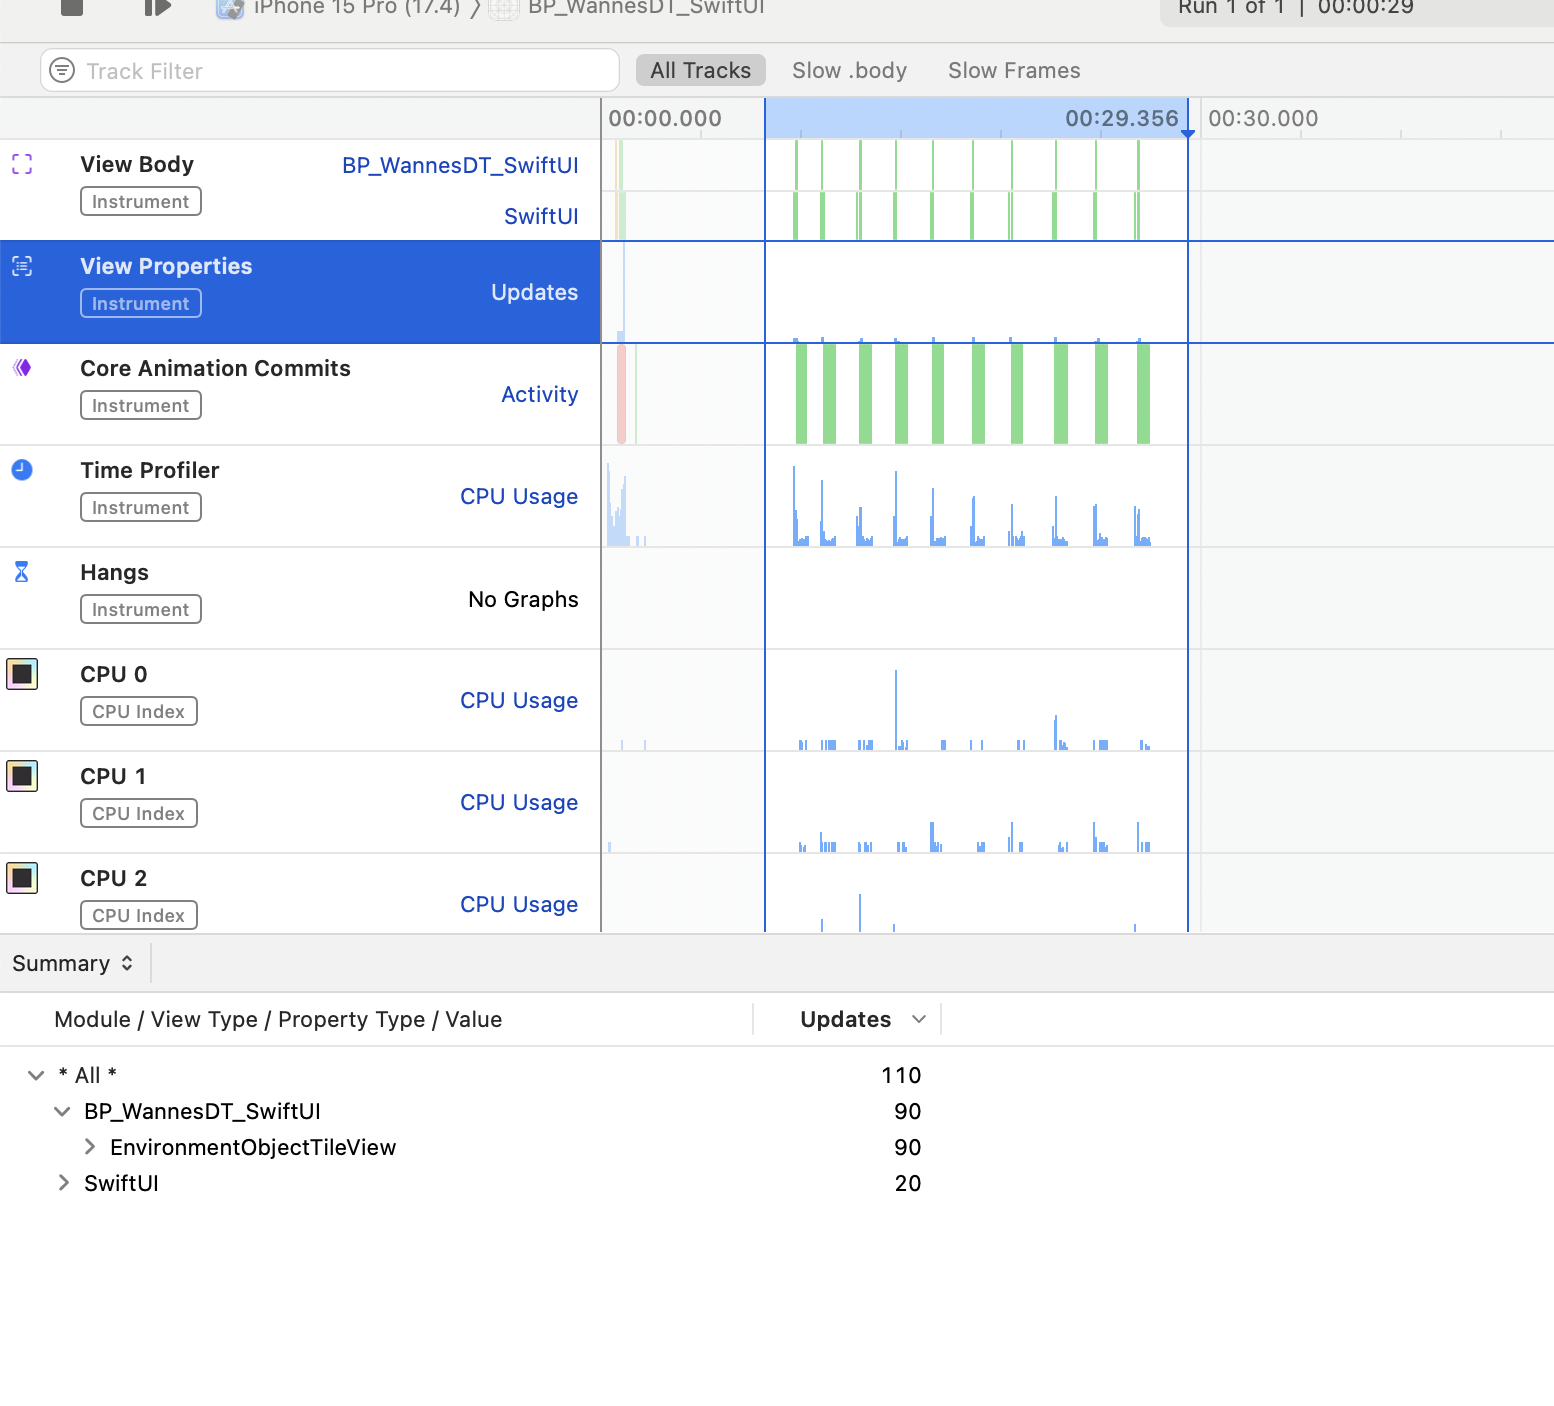
\includegraphics[width=0.7\textwidth]{BPtest2_lazy/EnvironmentObjectPropertyUpdates} 
    \caption{test3: Aantal keren dat de property's updaten bij het meervoudig toewijzigen van een EnvironmentObject}
    \label{fig:propertyUpdatesEnvironmentObject2}
\end{figure}
\paragraph{Totale tijd gebruikt van de CPU}
\begin{figure}[H]
    \centering
    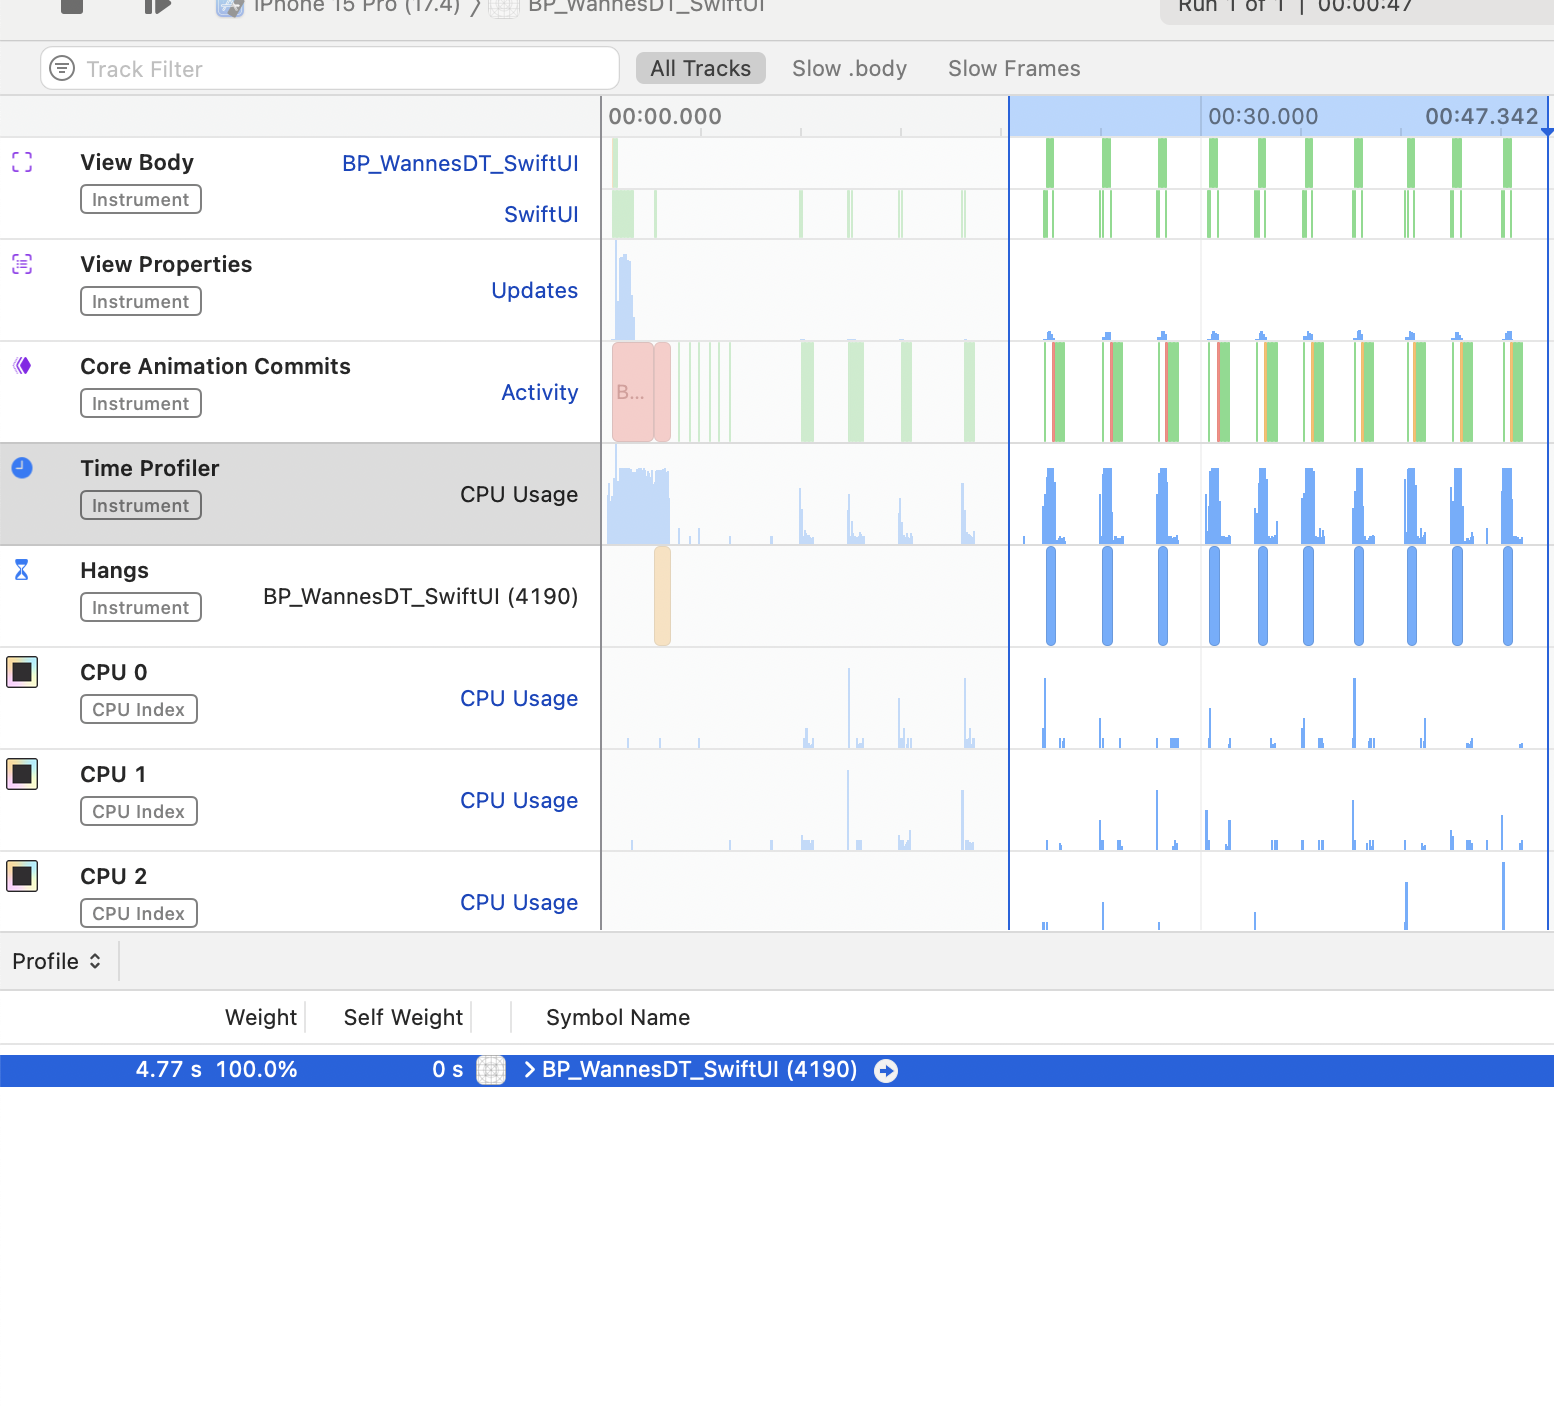
\includegraphics[width=0.7\textwidth]{BPtest2_lazy/EnvironmentObjectTotalCpuTime} 
    \caption{test3: De totale duratie die gebruikt is van de CPU bij het gebruik van EnvironmentObject's}
    \label{fig:cpuUsageTimeEnvironmentObject2}
\end{figure}
\paragraph{Last op de CPU}
\begin{figure}[H]
    \centering
    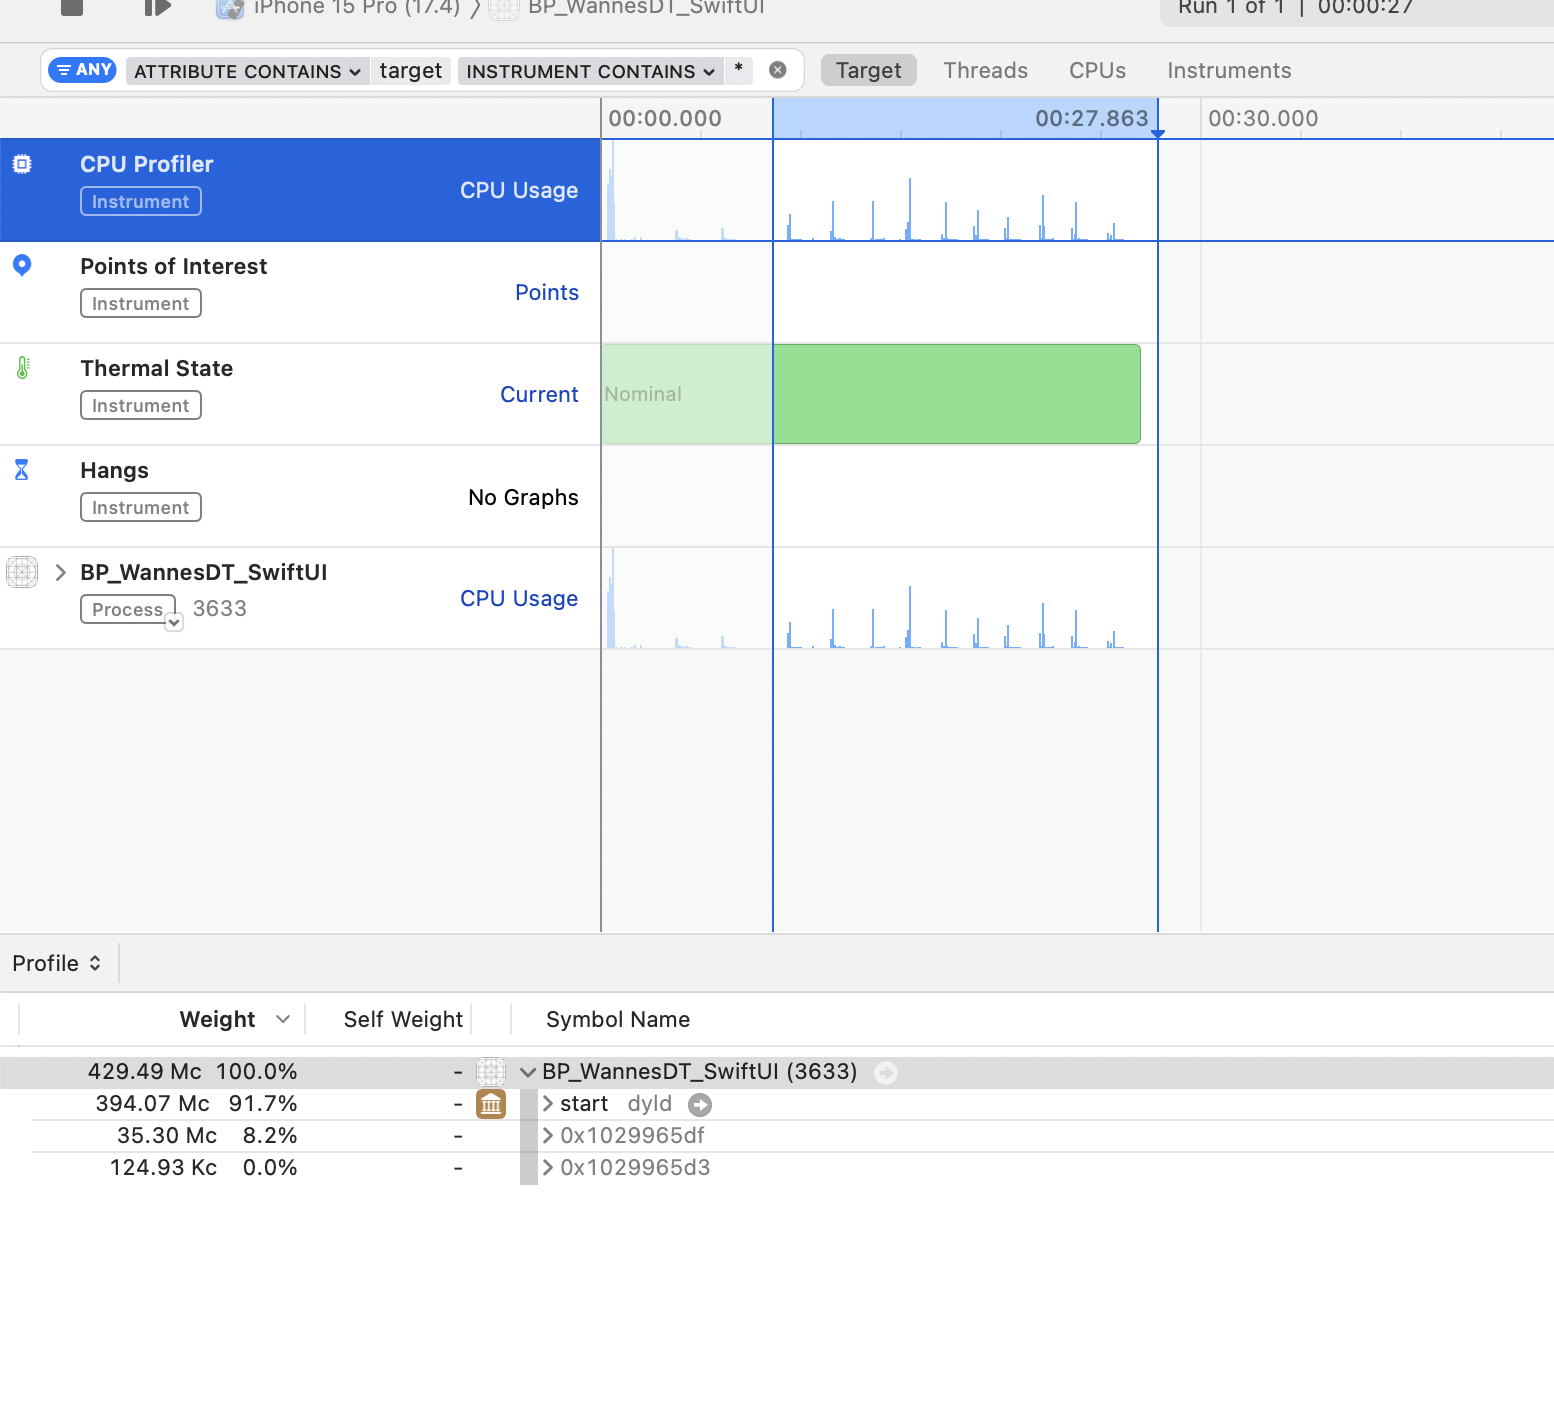
\includegraphics[width=0.7\textwidth]{BPtest2_lazy/EnvironmentObjectCpuWieght} 
    \caption{test3: De totale last van het opnieuw toewijzen van property's op de cpu bij het gebruik van EnvironmentObject's}
    \label{fig:cpuWeightEnvironmentObject2}
\end{figure}

\section{Test4: Dataoverdracht naar meerdere subview's}
% Binding test 3
In dit hoofdstuk word de applicatie in de afbeelding hieronder gebruikt om de testen uit te voeren. Opgebouwd uit 1 VStack's die 10 HStack's bevat per HStack worden er 10 Tegels weergegeven. Elke tegel is zeer CPU heavy opgebouwd zodat de resultaten meer zichtbaar worden in de testen. Elke tile bevat ook een knop die een aanpassing van de testbare data gaat triggeren. In volgende afbeelding word de hierarchy afgebeeld. Voor elk type van dataoverdracht is er 10 keer op de button gedrukt voor het wijzigen van de view. Zo zijn de metingen tot stand gekomen. Alle ruwe resultaten die waargenomen zijn per datatype kan u terugvinden in onderstaande sectie's en afbeeldingen.
\begin{figure}[htbp]
    \centering
    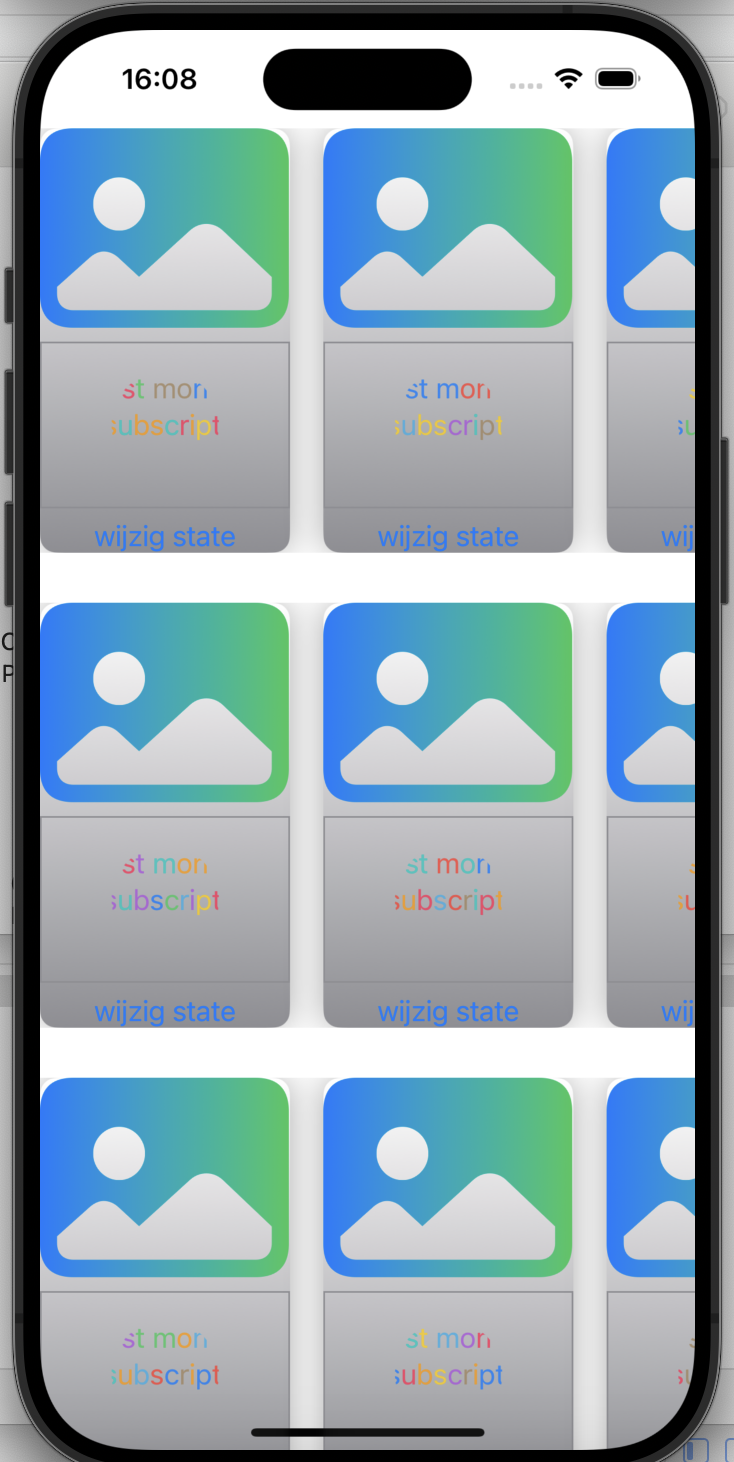
\includegraphics[width=0.4\textwidth]{testapplication} 
    \caption{testapplicatie}
    \label{fig:testapplication3}
\end{figure}
\begin{figure}[htbp]
    \centering
    \includegraphics[width=0.4\textwidth]{bptest2_lazy/dataHierarchy} 
    \caption{testapplicatie data hierarchy}
    \label{fig:testapplicationHierarchy3}
\end{figure}
\subsection{Binding}
\paragraph{View ververs aantal en ververs tijd}
\begin{figure}[H]
    \centering
    \includegraphics[width=0.7\textwidth]{BPtest2_notlazy/BindingViewRefreshes} 
    \caption{test4: Aantal keren dat de view refreshed en gemiddelde duratie bij het meervoudig toewijzigen van een binding}
    \label{fig:viewRefreshesBinding3}
\end{figure}
\paragraph{Aantal updates van property's}
\begin{figure}[H]
    \centering
    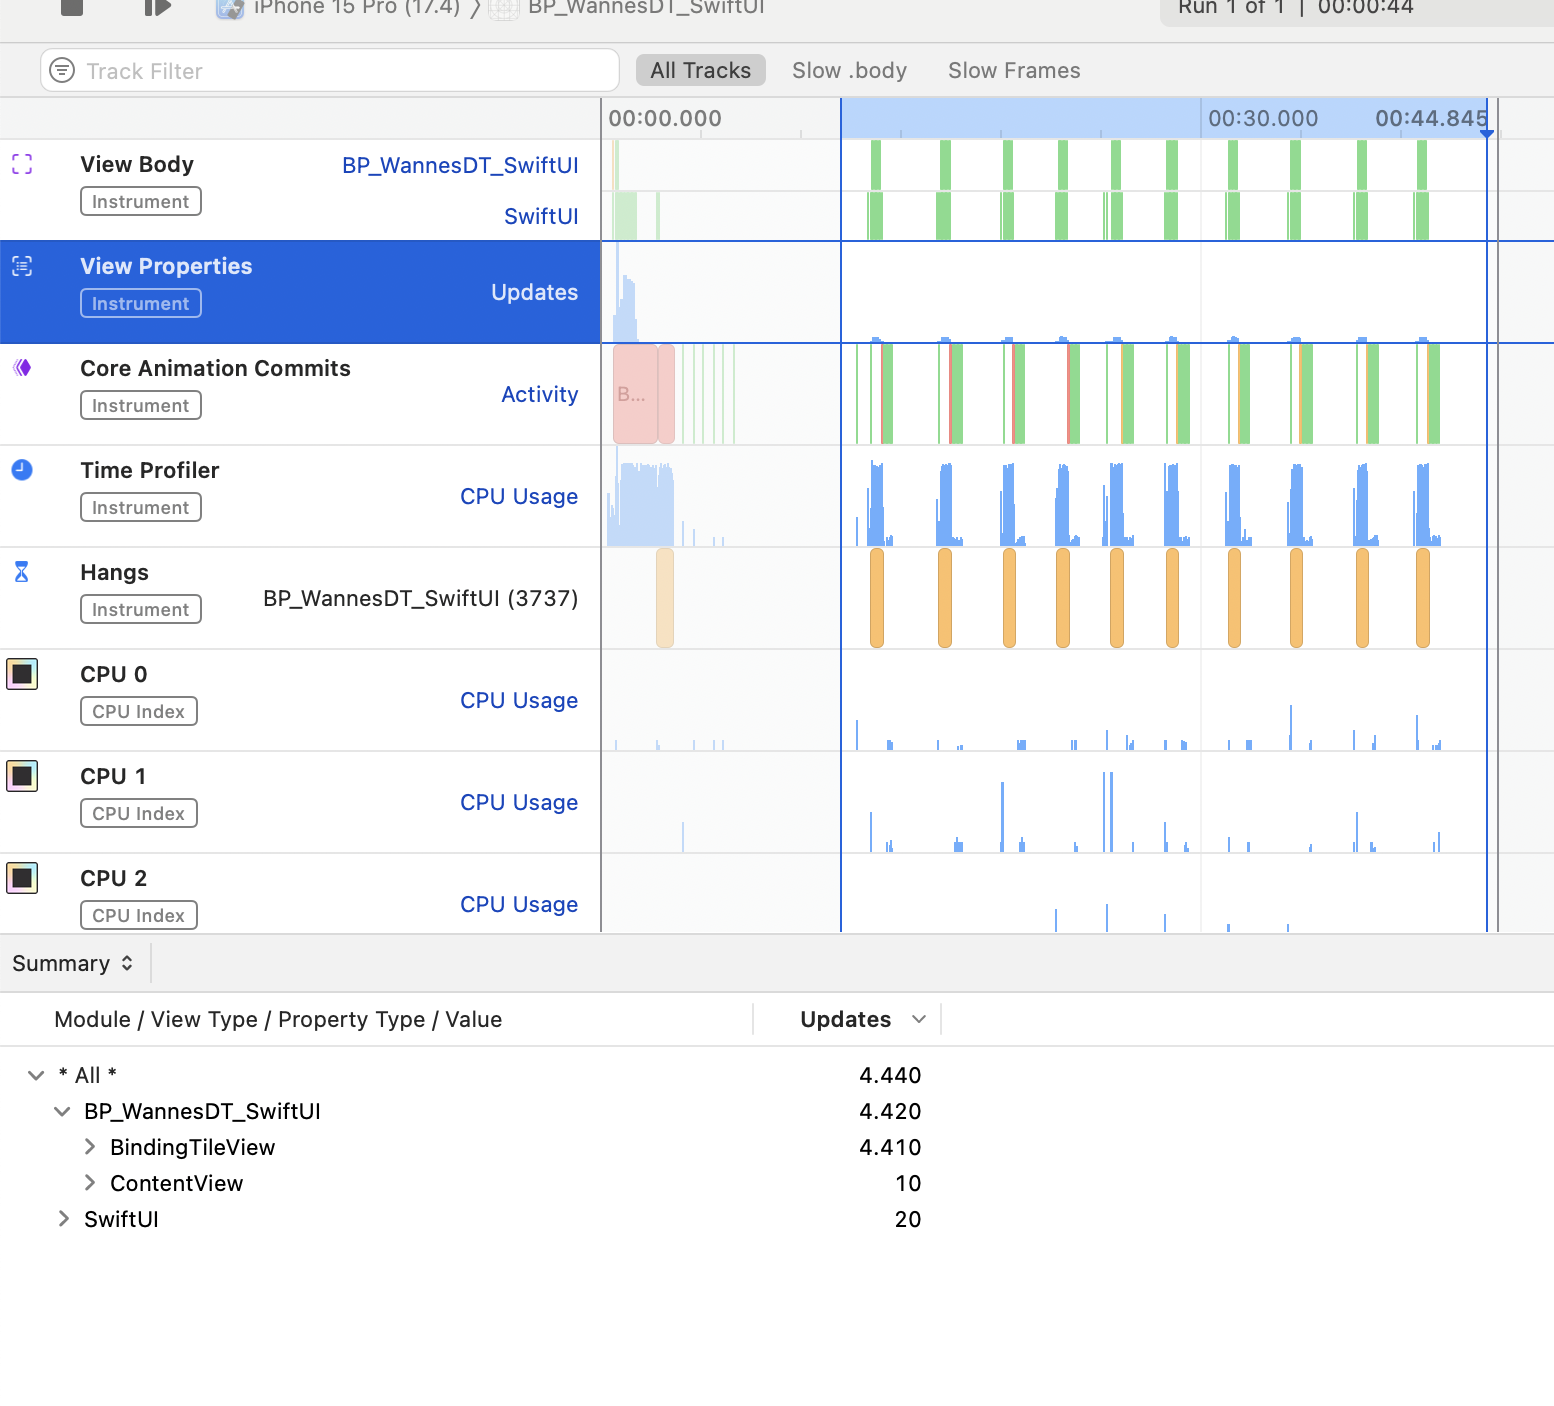
\includegraphics[width=0.7\textwidth]{BPtest2_notlazy/BindingViewPropertyUpdates} 
    \caption{test4: Aantal keren dat de property's updaten bij het meervoudig toewijzigen van een binding}
    \label{fig:propertyUpdatesBinding3}
\end{figure}
\paragraph{Totale tijd gebruikt van de CPU}
\begin{figure}[H]
    \centering
    \includegraphics[width=0.7\textwidth]{BPtest2_notlazy/BindingTotalCpuTime} 
    \caption{test4: De totale duratie die gebruikt is van de CPU bij het gebruik van bindings}
    \label{fig:cpuUsageTimeBinding3}
\end{figure}
\paragraph{Last op de CPU}
\begin{figure}[H]
    \centering
    \includegraphics[width=0.7\textwidth]{BPtest2_notlazy/BindingCpuWeight} 
    \caption{test4: De totale last van het opnieuw toewijzen van property's op de cpu bij het gebruik van bindings}
    \label{fig:cpuWeightBinding3}
\end{figure}

% Observable test 3
\subsection{Observable}
\paragraph{View ververs aantal en ververs tijd}
\begin{figure}[H]
    \centering
    \includegraphics[width=0.7\textwidth]{BPtest2_notlazy/ObservableViewRefreshes} 
    \caption{test4: Aantal keren dat de view refreshed en gemiddelde duratie bij het meervoudig toewijzigen van een Observable}
    \label{fig:viewRefreshesObservable3}
\end{figure}
\paragraph{Aantal updates van property's}
\begin{figure}[H]
    \centering
    \includegraphics[width=0.7\textwidth]{BPtest2_notlazy/ObservableViewPropertyUpdates} 
    \caption{test4: Aantal keren dat de property's updaten bij het meervoudig toewijzigen van een Observable}
    \label{fig:propertyUpdatesObservable3}
\end{figure}
\paragraph{Totale tijd gebruikt van de CPU}
\begin{figure}[H]
    \centering
    \includegraphics[width=0.7\textwidth]{BPtest2_notlazy/ObservableTotalCpuTime} 
    \caption{test4: De totale duratie die gebruikt is van de CPU bij het gebruik van Observable's}
    \label{fig:cpuUsageTimeObservable3}
\end{figure}
\paragraph{Last op de CPU}
\begin{figure}[H]
    \centering
    \includegraphics[width=0.7\textwidth]{BPtest2_notlazy/ObservableCpuWeight} 
    \caption{test4: De totale last van het opnieuw toewijzen van property's op de cpu bij het gebruik van Observable's}
    \label{fig:cpuWeightObservable3}
\end{figure}

% ObservedObject test 3
\subsection{ObservedObject}
\paragraph{View ververs aantal en ververs tijd}
\begin{figure}[H]
    \centering
    \includegraphics[width=0.7\textwidth]{BPtest2_notlazy/ObservedObjectViewRefreshes} 
    \caption{test4: Aantal keren dat de view refreshed en gemiddelde duratie bij het meervoudig toewijzigen van een ObservedObject}
    \label{fig:viewRefreshesObservedObject3}
\end{figure}
\paragraph{Aantal updates van property's}
\begin{figure}[H]
    \centering
    \includegraphics[width=0.7\textwidth]{BPtest2_notlazy/ObservedObjectViewPropertyUpdates} 
    \caption{test4: Aantal keren dat de property's updaten bij het meervoudig toewijzigen van een ObservedObject}
    \label{fig:propertyUpdatesObservedObject3}
\end{figure}
\paragraph{Totale tijd gebruikt van de CPU}
\begin{figure}[H]
    \centering
    \includegraphics[width=0.7\textwidth]{BPtest2_notlazy/ObservedObjectTotalCpuTime} 
    \caption{test4: De totale duratie die gebruikt is van de CPU bij het gebruik van ObservedObject's}
    \label{fig:cpuUsageTimeObservedObject3}
\end{figure}
\paragraph{Last op de CPU}
\begin{figure}[H]
    \centering
    \includegraphics[width=0.7\textwidth]{BPtest2_notlazy/ObservedObjectCpuWeight} 
    \caption{test4: De totale last van het opnieuw toewijzen van property's op de cpu bij het gebruik van ObservedObject's}
    \label{fig:cpuWeightObservedObject3}
\end{figure}

% EnvironmentObject test 3
\subsection{EnvironmentObject}
\paragraph{View ververs aantal en ververs tijd}
\begin{figure}[H]
    \centering
    \includegraphics[width=0.7\textwidth]{BPtest2_notlazy/EnvironmentObjectViewRefreshes} 
    \caption{test4: Aantal keren dat de view refreshed en gemiddelde duratie bij het meervoudig toewijzigen van een EnvironmentObject}
    \label{fig:viewRefreshesEnvironmentObject3}
\end{figure}
\paragraph{Aantal updates van property's}
\begin{figure}[H]
    \centering
    \includegraphics[width=0.7\textwidth]{BPtest2_notlazy/EnvironmentObjectViewPropertyUpdates} 
    \caption{test4: Aantal keren dat de property's updaten bij het meervoudig toewijzigen van een EnvironmentObject}
    \label{fig:propertyUpdatesEnvironmentObject3}
\end{figure}
\paragraph{Totale tijd gebruikt van de CPU}
\begin{figure}[H]
    \centering
    \includegraphics[width=0.7\textwidth]{BPtest2_notlazy/EnvironmentObjectTotalCpuTime} 
    \caption{test4: De totale duratie die gebruikt is van de CPU bij het gebruik van EnvironmentObject's}
    \label{fig:cpuUsageTimeEnvironmentObject3}
\end{figure}
\paragraph{Last op de CPU}
\begin{figure}[H]
    \centering
    \includegraphics[width=0.7\textwidth]{BPtest2_notlazy/EnvironmentObjectCpuWeight} 
    \caption{test4: De totale last van het opnieuw toewijzen van property's op de cpu bij het gebruik van EnvironmentObject's}
    \label{fig:cpuWeightEnvironmentObject3}
\end{figure}

\chapter{Resultaten}%
In dit hoofdstuk word er dieper in de onderzoeksresultaten van dit onderzoek gedelft. Alle resultaten zijn verkregen door de applicatie te testen via een Iphone 15 pro, IOS 17.4. Alle testen zijn ook systematisch 10 tot 100 keer overlopen voor een correcter resultaat. 


